
\section{Thông tin lớp học}
\begin{itemize}
    \item Phạm Thị Hồng Thơm / 096-770-1977 / 1977
    \item ? Quỳnh / 1977k
\end{itemize}

\newpage


\section{An toàn y tế}

\subsection{Quản lý rủi ro}

\begin{itemize}
    \item Cụ già cao tuổi loãng xương thì cần phải điều trị nhẹ nhàng.
    \item Dấu hiệu tê chân, tiểu tiện bất kiểm soát -> Cần khéo léo yêu cầu người bệnh đến cơ sở y tế để điều trị.
    \item Khi có sự cố -> Báo cáo cơ quan chức năng.
\end{itemize}

\subsection{Chính sách pháp luật}

\subsubsection{Vai trò lãnh đạo bệnh viện}
\begin{itemize}
    \item Cam kết, hỗ trợ, giám sát.
    \item Đào tạo định kỳ.
\end{itemize}

\subsection{Tổng kết}
An toàn y tế là trách nhiệm của mọi cá nhân. Cần sự phối hợp đa ngành.

\section{Giải phẫu}
\subsubsection{Trà}
Trà xanh có phenon. \\

Tác dụng trung hoà gốc tự do của phenon. Gốc tự do là các phân tử không ổn định, thiếu điện tử nên có xu hướng tranh chấp điện tử từ các tế bào khác, gây tổn thương tế bào. Việc phenon nhường điện tử giúp vô hiệu hoá các gốc tự do này, bảo vệ tế bào khỏi quá trình oxy hoá. \\

Gốc tự do là các phân tử, nguyên tử hoặc ion có một hoặc nhiều điện tử ở lớp vỏ ngoài cùng.

\subsection{Giải phẫu - sinh lý hệ xương}
Các mặt bẳng cơ thể.
Mặt phẳng ngang.
Vị trí gần xa, gần nội tạng xa gốc chi. Gốc chi đến ngọn chi (khớp tay khưy tay đến ngón tay, chân từ gốc chân, đến ...).
Bấm huyệt từ ngọn chi lại gần.
Trong ngoài, trên dưới.
Kinh âm chạy ở mặt trong và trước
Kinh dương chạy ở mặt ngoài và mặt sau.
Có một số kinh chạy bắt chéo.
Trước là phía bụng, sau là lưng.
Trên là đầu. dưới là chân.

Chức năng bộ xương.
\begin{enumerate}
    \item Duy trì chức năng cơ thể
    \item Xương chứa tuỷ đỏ tạo máu. Chủ yếu xương dẹt - tuỷ đỏ (xương sườn, bả vai, xương hậu).
    \item Bệnh về xương (loãng xương). Hạ canxi máu.
\end{enumerate}

Phân loại xương.
\begin{enumerate}
    \item Xương dài. Tối ưu hoá đòn bẩy.
    \item Xương ngắn (khối đa diện, chiều dài rộng tương đương nhau, Xuơng cổ tay, cổ chân). Tối ưu hoá độ chắc trong cử động.
    \item Xương tự do (xương bánh chè)
\end{enumerate}

\begin{enumerate}
    \item Xương dẹt. Xương sọ, bả vai, ức, xườn bảo vệ não, nội tạng
    \item Xương vừng. Nhỏ nằm trong gân, giamr ma sát (xương bánh chè)
    \item Xương không đều. đốt sống.
\end{enumerate}

Xương nối với nhau bằng cơ.

Khớp có dây chằng và gân.
\subsubsection{Cấu tạo đại thể xương dài}
Màng ngoài xương (màng bộc xương, nuôi dưỡng phát triển, và hàn gắn khi gẫy)
Sụn khớp nhẵn bọc đầu xương giảm ma xát khi cử động.
Mô xương đặc lớp ngoài trong thì xốp. Bên trong có chứa ống tuỷ xương. Xương dài tuỷ vàng dẹt tuỷ đỏ.

Xương đặc.
Xương sốp. Giảm trọng lượng bộ xương đảm bảo độ bề vững.

Thành phần hoá học 70\% khoáng chất và chất vô cơ. 30\% là chất hữu cơ tạo sự dẻo dai.

Quá trình hình thành và phát triển của xương.
Cốt hoá, thay thế lớp màng và sụn tạo thành mô xương cứng.

\subsection{Quá trình tái tạo và liền xương.}
Cơ thể tự chữa lành.

\subsubsection{Đại cương về hệ xương}

\section{Quá trình tái tạo và liền xương}

Quá trình liền xương là một chuỗi phản ứng sinh học phức tạp giúp phục hồi cấu trúc và chức năng của xương sau chấn thương, gồm 4 giai đoạn chính:

\subsection{Các giai đoạn liền xương}

\begin{enumerate}
    \item \textbf{Giai đoạn tụ máu (Viêm cấp tính - 1 đến 7 ngày):}
    \begin{itemize}
        \item Mạch máu tại ổ gãy bị đứt sinh ra khối máu tụ (hematoma).
        \item Giải phóng các yếu tố tăng trưởng và huy động tế bào viêm, đại thực bào đến dọn dẹp mô hoại tử.
    \end{itemize}

    \item \textbf{Giai đoạn can xương mềm (1 đến 3 tuần):}
    \begin{itemize}
        \item Các tế bào trung mô biệt hóa thành nguyên bào sợi và nguyên bào sụn.
        \item Tạo ra mô liên kết và sụn mềm liên kết hai đầu xương gãy lại với nhau.
    \end{itemize}

    \item \textbf{Giai đoạn can xương cứng (2 đến 4 tháng):}
    \begin{itemize}
        \item Quá trình cốt hóa xuất hiện, thay thế mô sụn mềm thành mô xương xốp (can xương cứng).
        \item Ổ gãy bắt đầu vững chắc về mặt cơ học.
    \end{itemize}

    \item \textbf{Giai đoạn tái cấu trúc (Mấy tháng đến vài năm):}
    \begin{itemize}
        \item Sự phối hợp giữa hủy xương bào (xóa bỏ xương thừa) và tạo xương bào (sắp xếp lại cấu trúc).
        \item Xương khôi phục lại hình dạng, đường lực và độ chắc ban đầu.
    \end{itemize}
\end{enumerate}

\subsection{Yếu tố ảnh hưởng đến quá trình liền xương}

\begin{itemize}
    \item \textbf{Yếu tố tại chỗ:} Sự bất động ổ gãy, mức độ tổn thương phần mềm, nguồn cung cấp máu và tình trạng nhiễm trùng.
    \item \textbf{Yếu tố toàn thân:} Tuổi tác, dinh dưỡng (Calci, Vitamin D, Protein), bệnh lý nền (loãng xương, tiểu đường) và các thói quen như hút thuốc lá.
\end{itemize}

\section{Cấu trúc tổng thể của bộ xương}
% Xương sọ
\begin{figure}
    \centering
    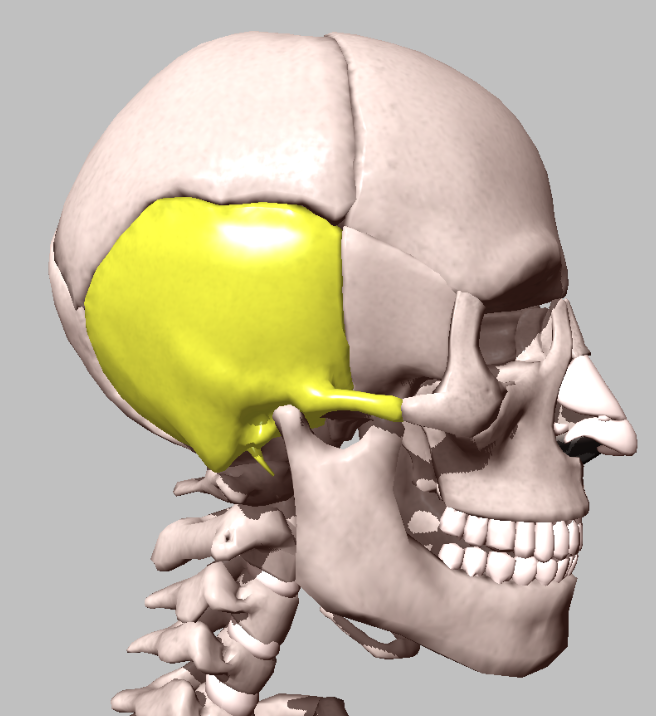
\includegraphics[width=0.5\linewidth]{images/xương sọ.png}
    \caption{Enter Caption}
    \label{fig:placeholder}
\end{figure}
% - Cứng nhất
% Xương măt
\begin{figure}
    \centering
    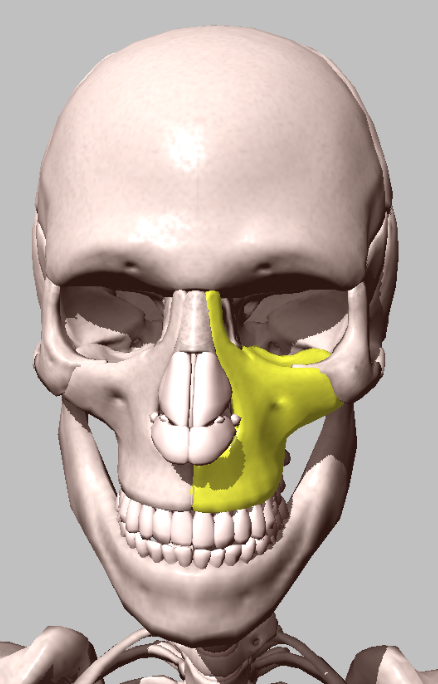
\includegraphics[width=0.5\linewidth]{images/xương mặt.png}
    \caption{Enter Caption}
    \label{fig:placeholder}
\end{figure}
% xương cột sống.
\begin{figure}
    \centering
    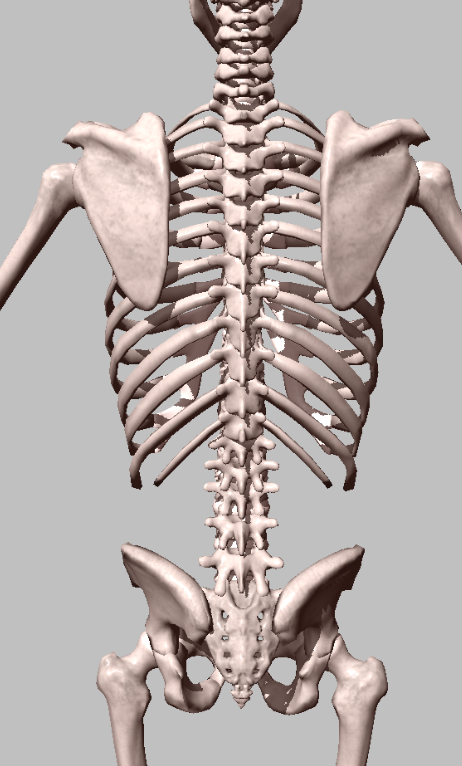
\includegraphics[width=0.5\linewidth]{images/xương cột sống.png}
    \caption{Enter Caption}
    \label{fig:placeholder}
\end{figure}
% đốt sống cổ
\begin{figure}
    \centering
    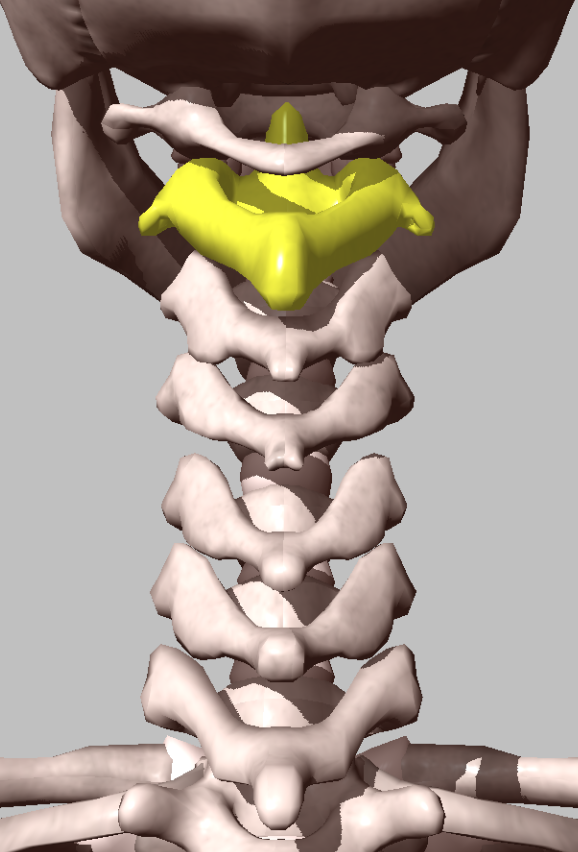
\includegraphics[width=0.5\linewidth]{images/đốt sống cổ.png}
    \caption{Enter Caption}
    \label{fig:placeholder}
\end{figure}
\begin{figure}
    \centering
    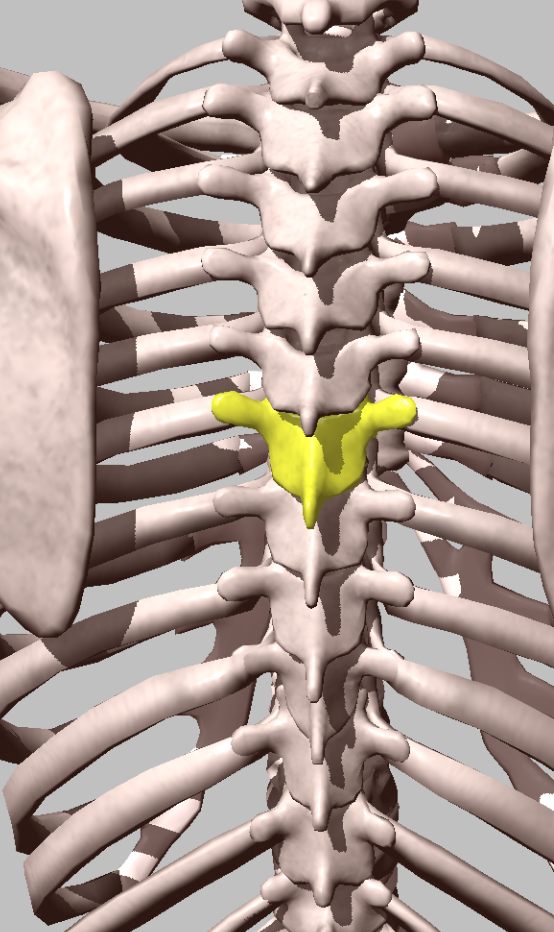
\includegraphics[width=0.5\linewidth]{images/lưng 1.png}
    \caption{Enter Caption}
    \label{fig:placeholder}
\end{figure}
% Xương trục
% Xươngg phụ

\section{Bệnh lý xương}
\subsection{Bệnh loãng xương}
% dòn dễ gãy
% viêm xương khớp
% đau khớp cứng khớp, hạn chế vận động
\subsection{Gãy xương}
% biến dạng chi
% sưng đau, mất chức năng vận động.

\section{Khí công}

\section{Xoa bóp}

\begin{table}[H]
    \centering
    \begin{tabular}{|c|c|c|c|c|}
        \hline
        ID & Tên động tác & Cơ quan & Quỹ đạo & Ghi chú
        \\ \hline
        1 & Xát & Ngón cái | Ngón út | Gốc bàn tay & Lên xuống | Trái phải & Thông khí, Giảm sưng
        \\ \hline
        2 & Xoa & Ngón cái | Mô út | Gốc bàn tay & Đường tròn & Chậm, nhẹ
        \\ \hline
        3 & Miết & Ngón cái & Trên xuống | Dưới lên | Phải sang Trái | Trái sang Phải & 
        \\ \hline
    \end{tabular}
    \caption{Caption}
    \label{tab:placeholder}
\end{table}


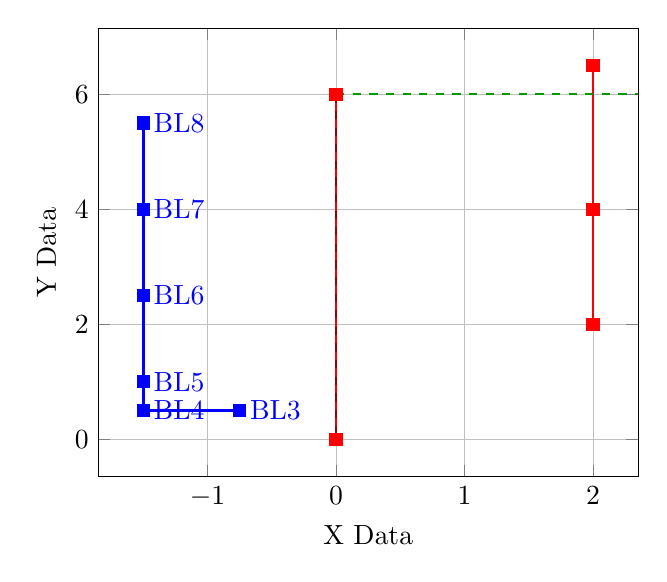
\begin{tikzpicture}
    \begin{axis}[
        xlabel={X Data},
        ylabel={Y Data},
        grid=both
    ]
        \addplot[
            color=red,
            mark=square*,
            thick
        ] coordinates {
            (2, 2)
            (2, 4)
            (2, 6.5)
        };
        
        \addplot[
            color=red,
            mark=square*,
            thick
        ] coordinates {
            (0, 0)
            (0, 6)
        };

        \addplot[
            color=blue,
            mark=square*,
            thick,
            nodes near coords,
            point meta=explicit symbolic,
            every node near coord/.append style={right}
        ] coordinates {
            (-0.75, 0.5) [BL3]
            (-1.5, 0.5) [BL4]
            (-1.5, 1) [BL5]
            (-1.5, 2.5) [BL6]
            (-1.5, 4.0) [BL7]
            (-1.5, 5.5) [BL8]
        };
        
        \draw[green!60!black, dashed, thick] (axis cs:0,6) -- (axis cs:6,6);

        \draw[red!60!black, dashed, thick] (axis cs:0,6) -- (axis cs:0,0);
    \end{axis}
\end{tikzpicture}



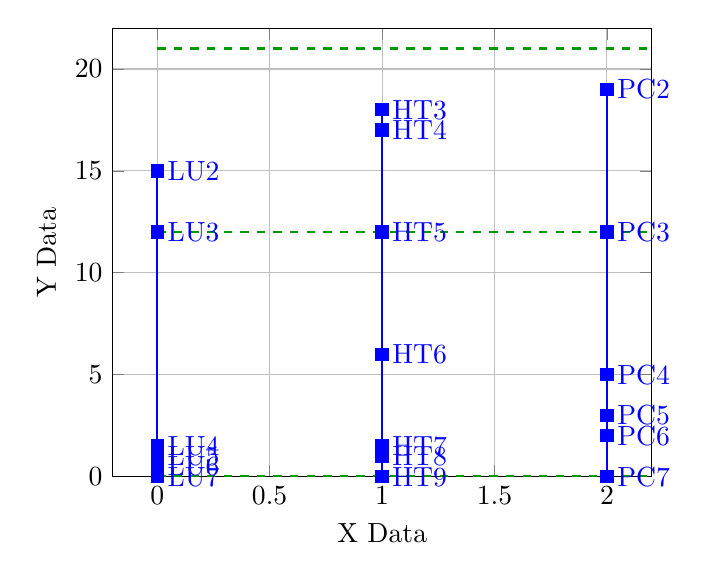
\begin{tikzpicture}
    \begin{axis}[
        xlabel={X Data},
        ylabel={Y Data},
        grid=both,
        ymin=0,
        ymax=22
    ]
        \addplot[
            color=blue,
            mark=square*,
            thick,
            nodes near coords,
            point meta=explicit symbolic,
            every node near coord/.append style={right}
        ] coordinates {
            (0, 0) [LU7]
            (0, 0.5) [LU6]
            (0, 1) [LU5]
            (0, 1.5) [LU4]
            (0, 12) [LU3]
            (0, 15) [LU2]            
        };

        \addplot[
            color=blue,
            mark=square*,
            thick,
            nodes near coords,
            point meta=explicit symbolic,
            every node near coord/.append style={right}
        ] coordinates {
            (1, 0) [HT9]
            (1, 1) [HT8]
            (1, 1.5) [HT7]
            (1, 6) [HT6]
            (1, 12) [HT5]
            (1, 17) [HT4]
            (1, 18) [HT3]
        };

        \addplot[
            color=blue,
            mark=square*,
            thick,
            nodes near coords,
            point meta=explicit symbolic,
            every node near coord/.append style={right}
        ] coordinates {
            (2, 0) [PC7]
            (2, 2) [PC6]
            (2, 3) [PC5]
            (2, 5) [PC4]
            (2, 12) [PC3]
            (2, 19) [PC2]
        };
        
        \draw [green!60!black, dashed, thick] (axis cs:0, 21) -- (axis cs:6, 21);
        \draw [green!60!black, dashed, thick] (axis cs:0, 12) -- (axis cs:6, 12);
        \draw [green!60!black, dashed, thick] (axis cs:0, 0) -- (axis cs:6, 0);
    \end{axis}
\end{tikzpicture}

\section{Huyệt vị}
Xoa bóp bấm huyệt liên quan đến một từ gọi là \textbf{khí}.
Liên quan đến thứ hai là cảm giác đau trong cơ thể.

C1, C2 -> Đau đầu
C3 -> Cổ
C4 -> Đau vai
C5 -> Tay
C6 - Ngón cái, ngón trỏ
C7 -> Ngón giữa, ngón út

Thần kinh ngoại vi -> Chi phối hoạt động của tạng phủ
-> Cột sống quan trọng.

\begin{table}[]
    \centering
    \begin{tabular}{|c|c|c|}
        \hline
        Huyệt & Đốt sống lưng & 1.5 cun
        \\ \hline
        BL17 & T7 & 1.5 cun
        \\ \hline
        BL18 & T9 & 1.5 cun
        \\ \hline
        BL19 & T10 & 1.5 cun
        \\ \hline
        BL20 & T11 & 1.5 cun
        \\ \hline
        BL21 & T12 & 1.5 cun
        \\ \hline
        BL22 & L1 & 1.5 cun
        \\ \hline
        BL23 & L2 & 1.5 cun
        \\ \hline
        BL24 & L3 & 1.5 cun
        \\ \hline
        BL25 & L4 & 1.5 cun
        \\ \hline
        BL26 & L5 & 1.5 cun
        \\ \hline
        BL27 & 1st & 1.5 cun
        \\ \hline
        BL28 & 2st & 1.5 cun
        \\ \hline
        BL29 & 3st & 1.5 cun
        \\ \hline
        BL30 & 4st & 1.5 cun
        \\ \hline
    \end{tabular}
    \caption{Caption}
    \label{tab:placeholder}
\end{table}

\section{Trị liệu}

\subsection{Đau đầu}

\begin{table}[H]
    \centering
    \begin{tabular}{|p{1cm}|p{1cm}|p{2cm}|p{4cm}|p{4cm}|}
        \hline
         Step & Số lần & Action & Place & Ghi chú
         \\ \hline
         1 & Miết & - & Chân mày -> Thái dương, hết vùng chán &
         \\ \hline
         2 & Miết & 3 & Ấn đường -> Thái dương -> Đầu -> Phong trì &
         \\ \hline
         3 & Phân hợp & 5 to 10 & Vùng trán &
         \\ \hline
         4 & Vỗ & 3 vòng & Đầu & Hai bàn tay để đối diện nhau và vỗ xung quanh đầu một lực như nhau
         \\ \hline
         5 & Gõ & 3 vòng & Đầu & Hai tay đối diện, lực đều
         \\ \hline
         6 & Bấm & 1 & Bách hội, phong trì,  đầu duy, xuất cốc, thái dương. &
         \\ \hline
         7 & Chải & 1 & Đầu & Xoè 5 đầu ngón tay trải từ trước ra sau ra hai bên.
         \\ \hline
    \end{tabular}
    \caption{Cách động tác để chữa đau đầu}
    \label{tab:placeholder}


\end{table}

\begin{figure}
    \centering
    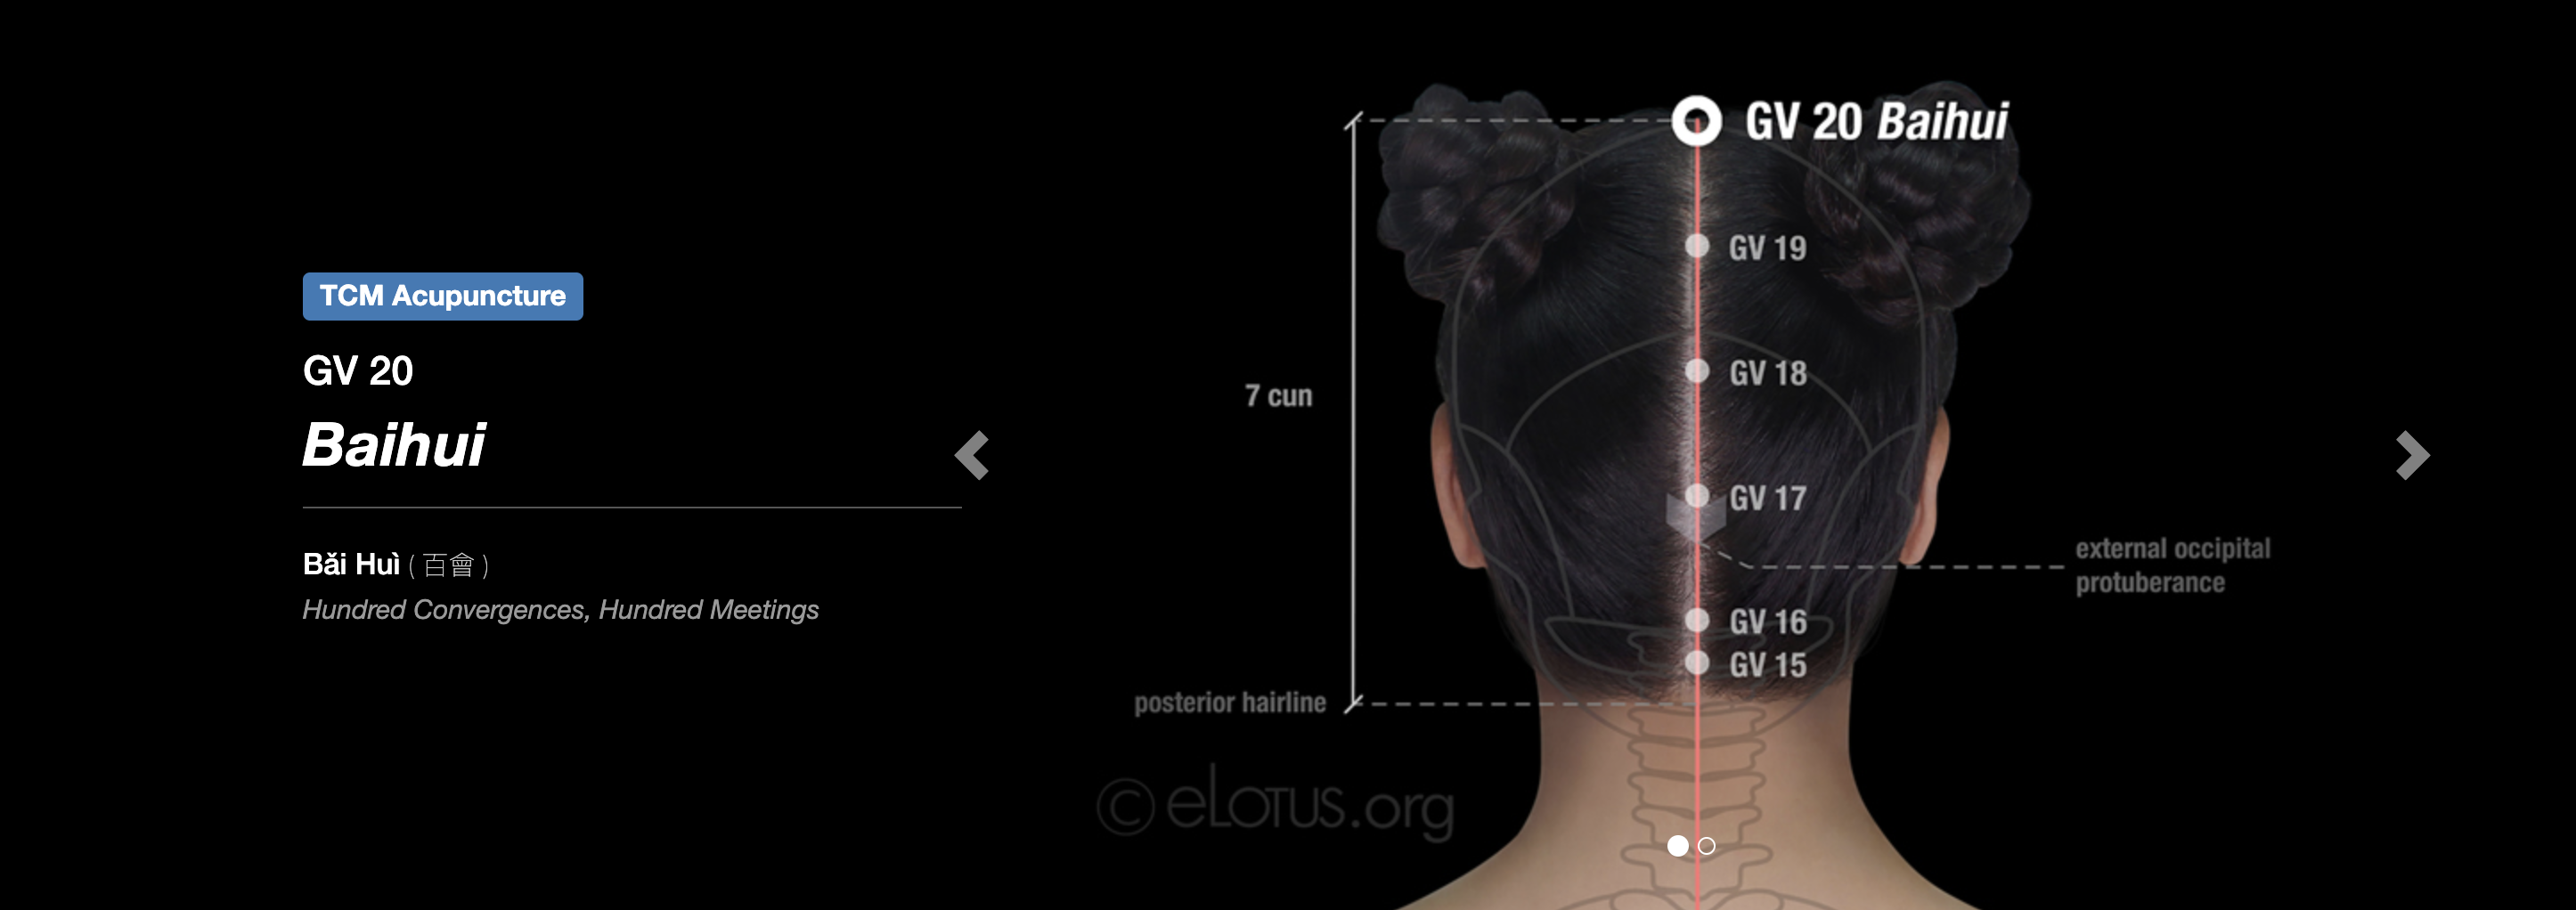
\includegraphics[width=\linewidth]{images/gv20a.png}
    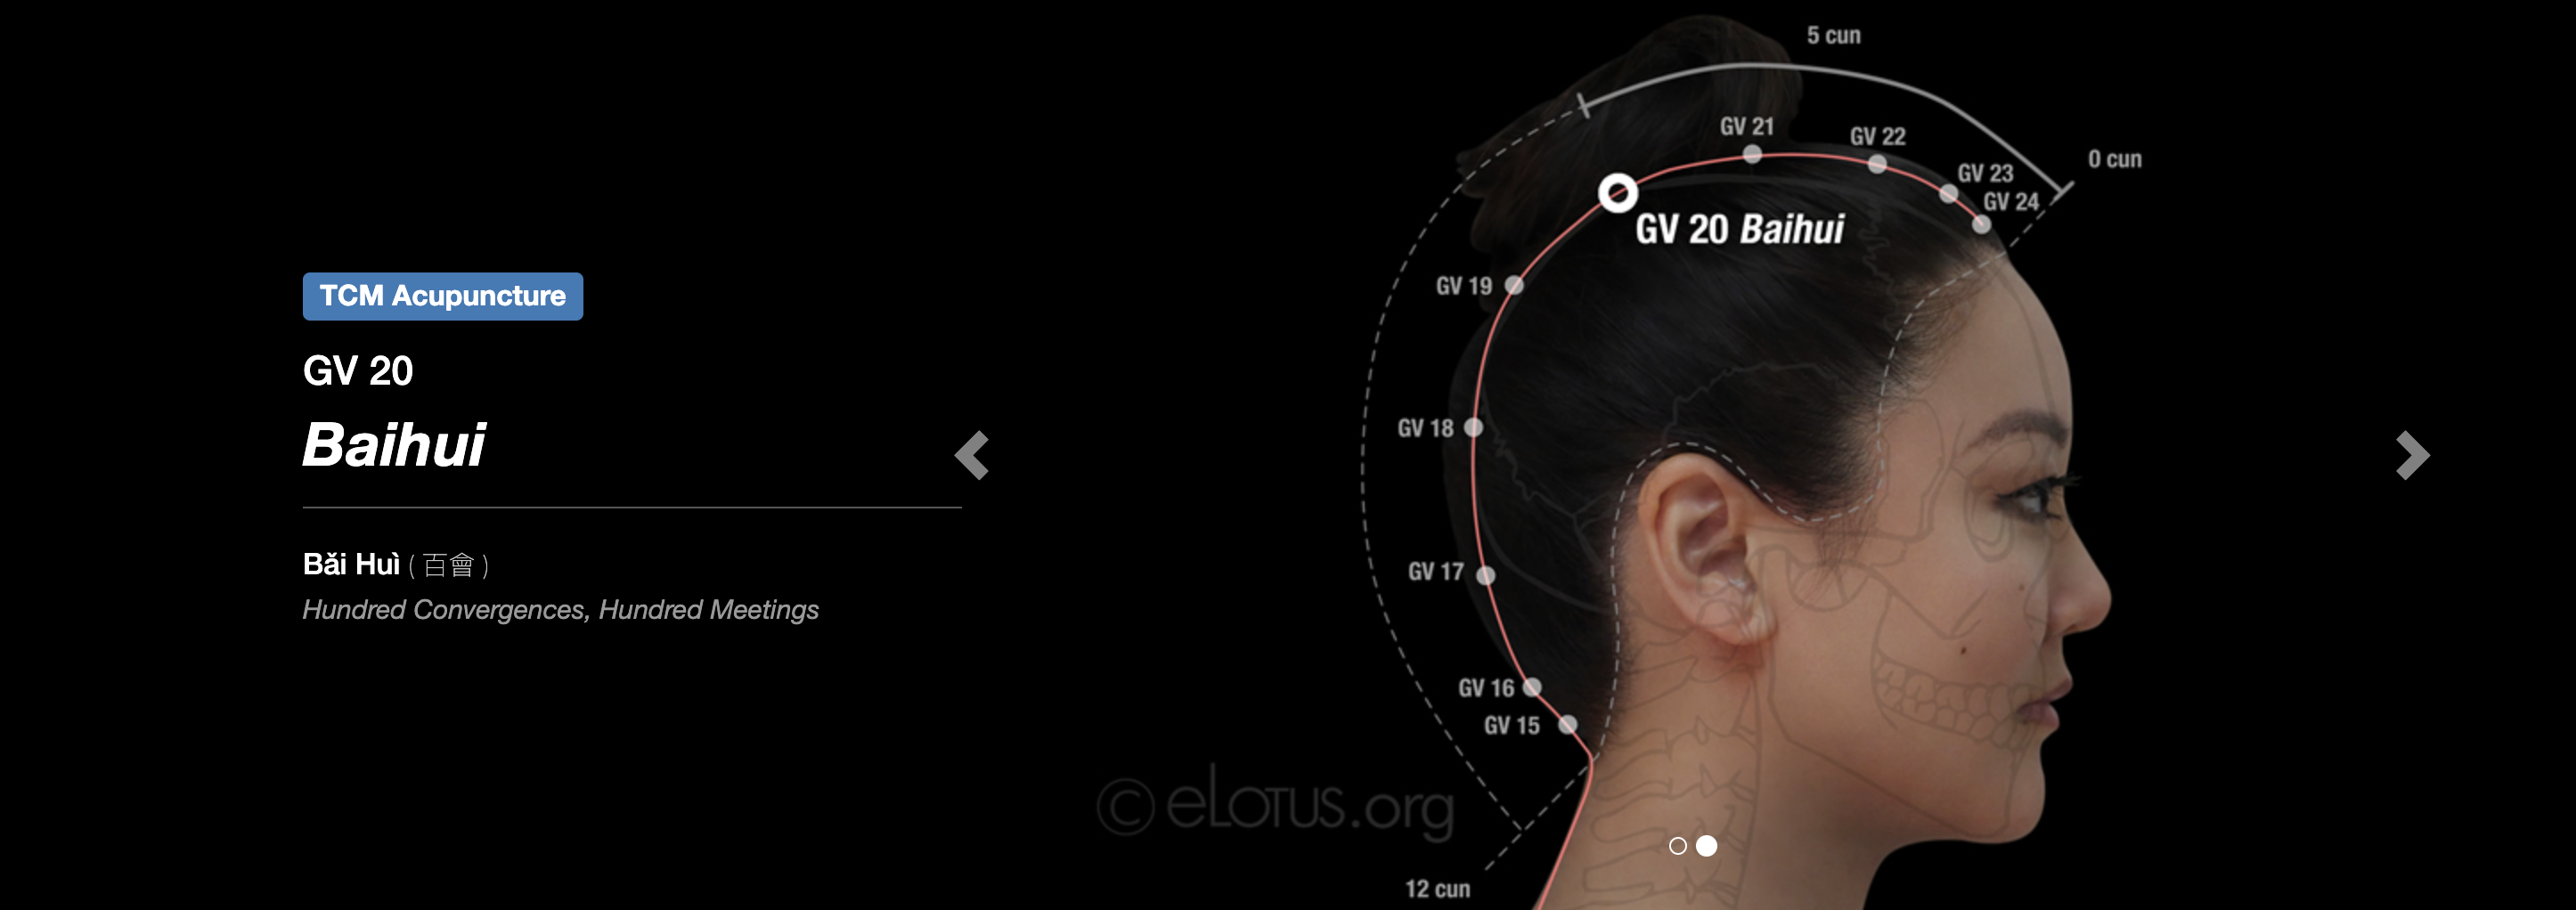
\includegraphics[width=\linewidth]{images/gv20b.png}
    \caption{Huyệt bách hội}
    \label{fig:placeholder}
\end{figure}

\begin{figure}
    \centering
    \includegraphics[width=1\linewidth]{images/ex-hn3.png}
    \caption{Huyệt ấn đường}
    \label{fig:placeholder}
\end{figure}

\begin{figure}
    \centering
    \includegraphics[width=1\linewidth]{images/ex-hn5.png}
    \caption{Huyệt thái dương}
    \label{fig:placeholder}
\end{figure}

\begin{figure}
    \centering
    \includegraphics[width=1\linewidth]{images/gb20.png}
    \caption{Huyệt phong trì}
\end{figure}

\begin{figure}
    \centering
    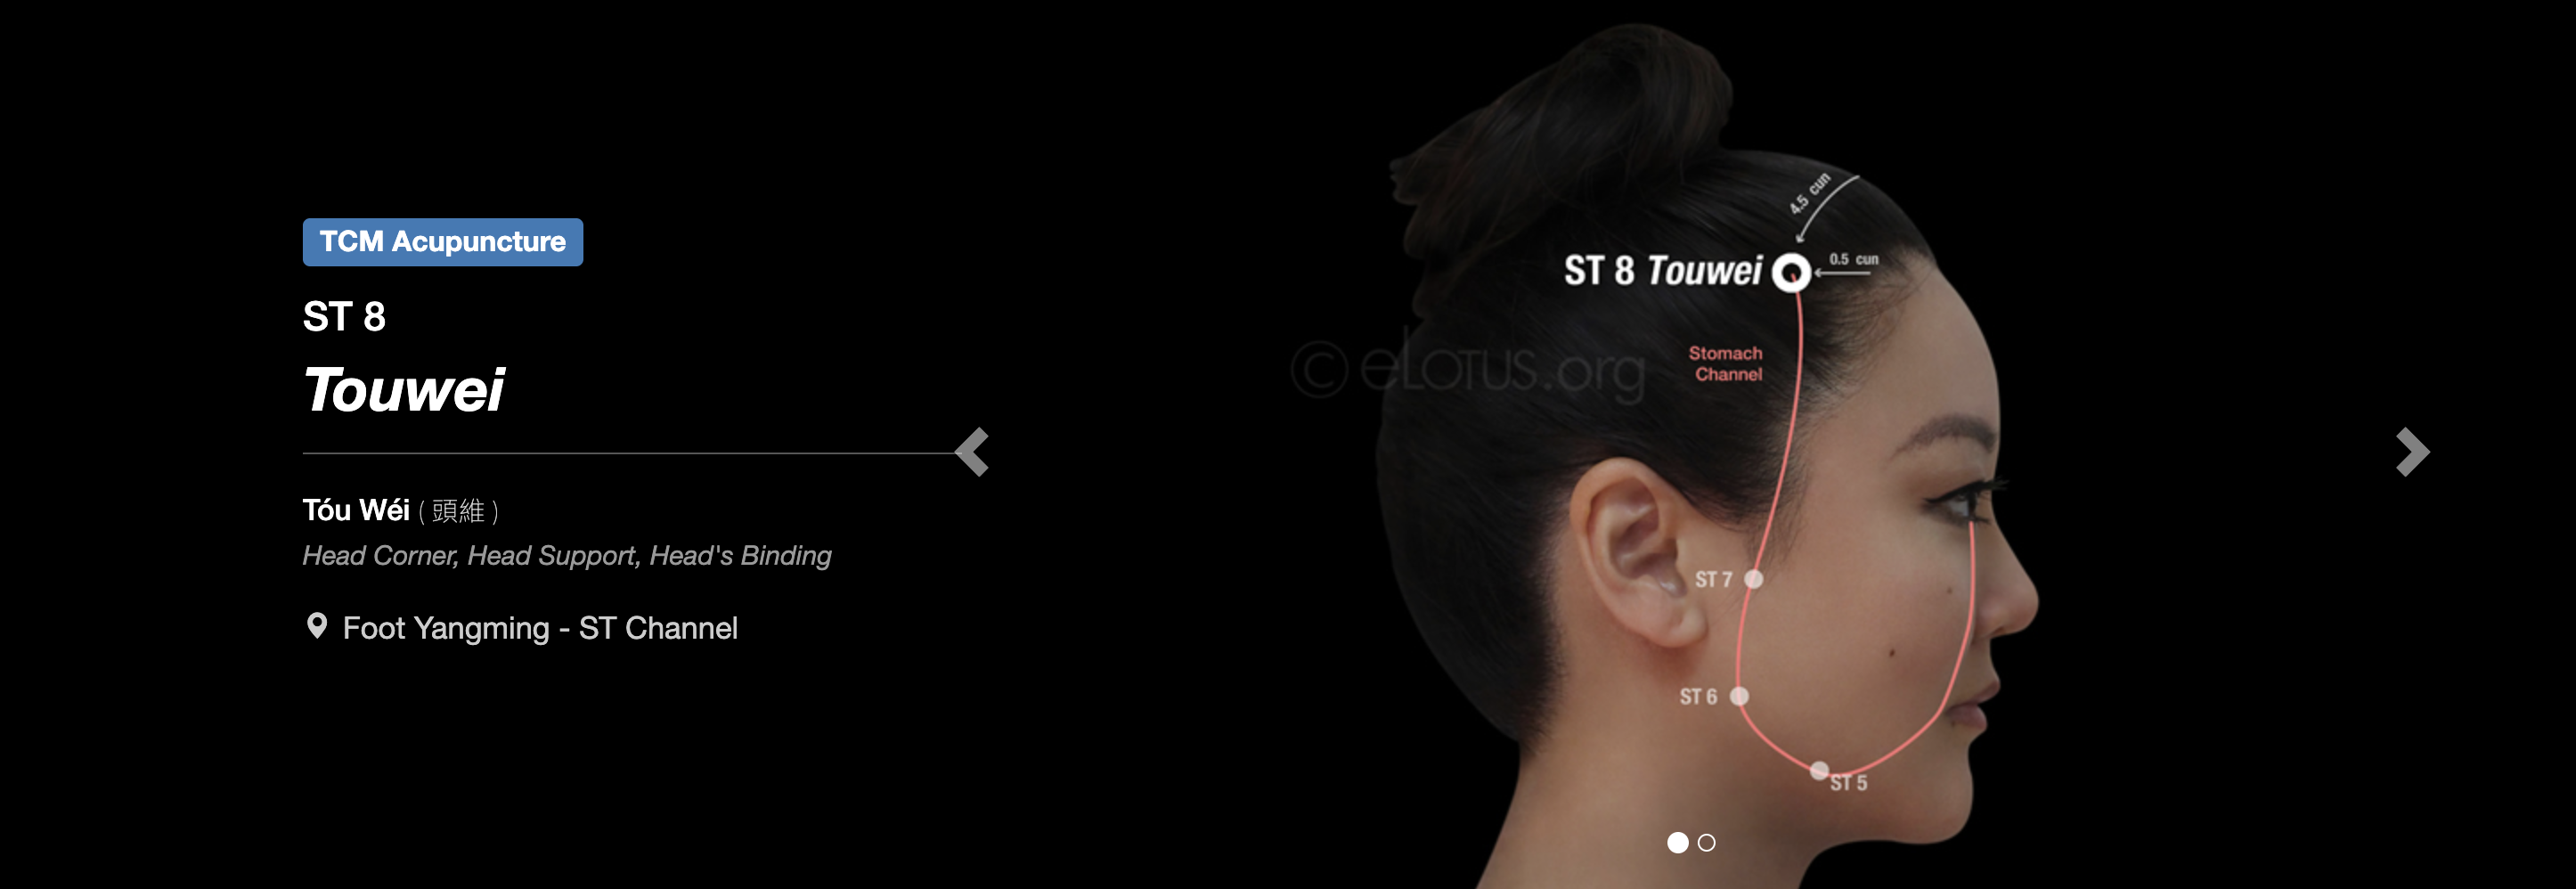
\includegraphics[width=1\linewidth]{images/st8a.png}
    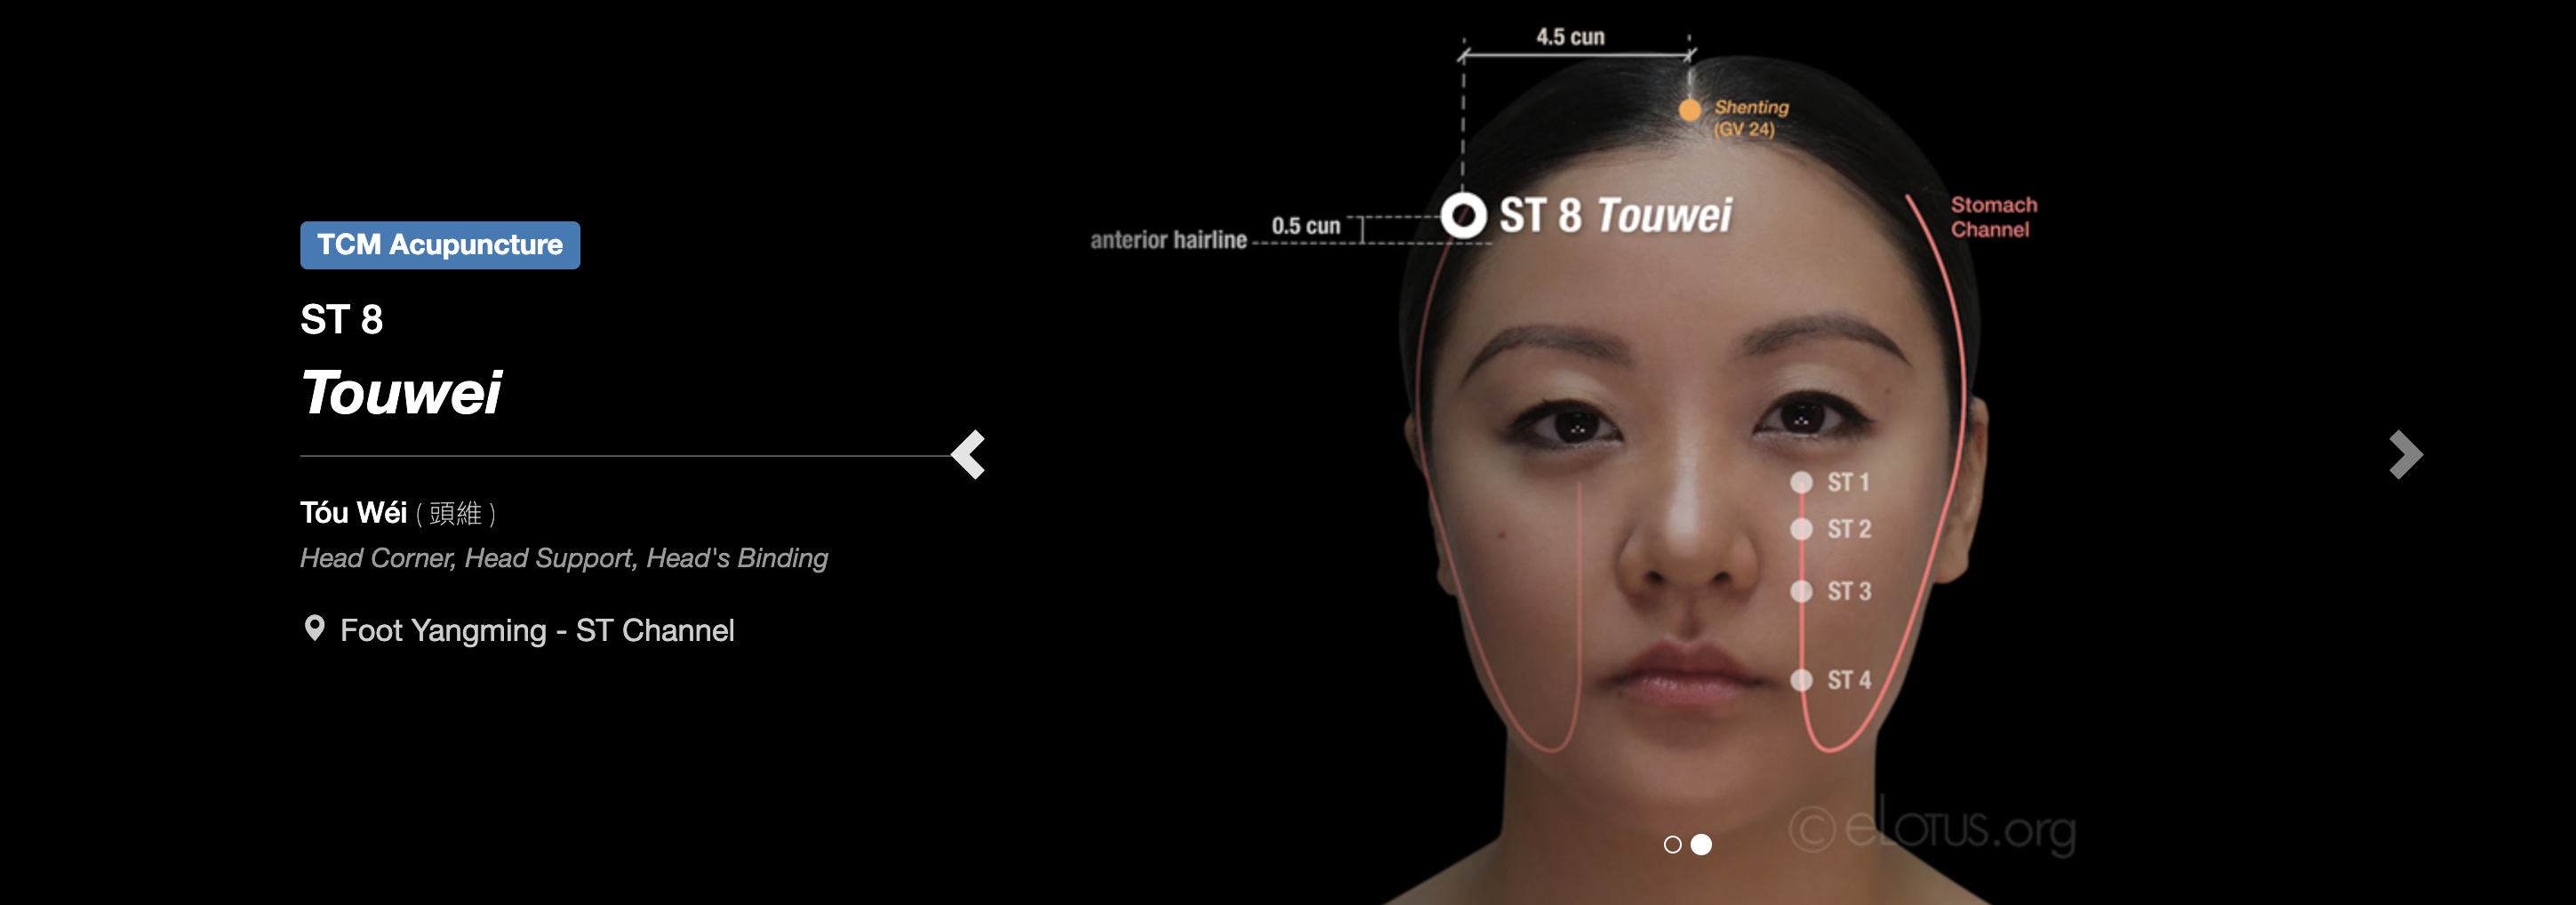
\includegraphics[width=1\linewidth]{images/st8b.png}
    \caption{Huyệt đầu duy}
    \label{fig:placeholder}
\end{figure}

\begin{figure}
    \centering
    \includegraphics[width=1\linewidth]{images/gb8.png}
    \caption{Huyệt Suất Cốc}
    \label{fig:placeholder}
\end{figure}

\begin{figure}
    \centering
    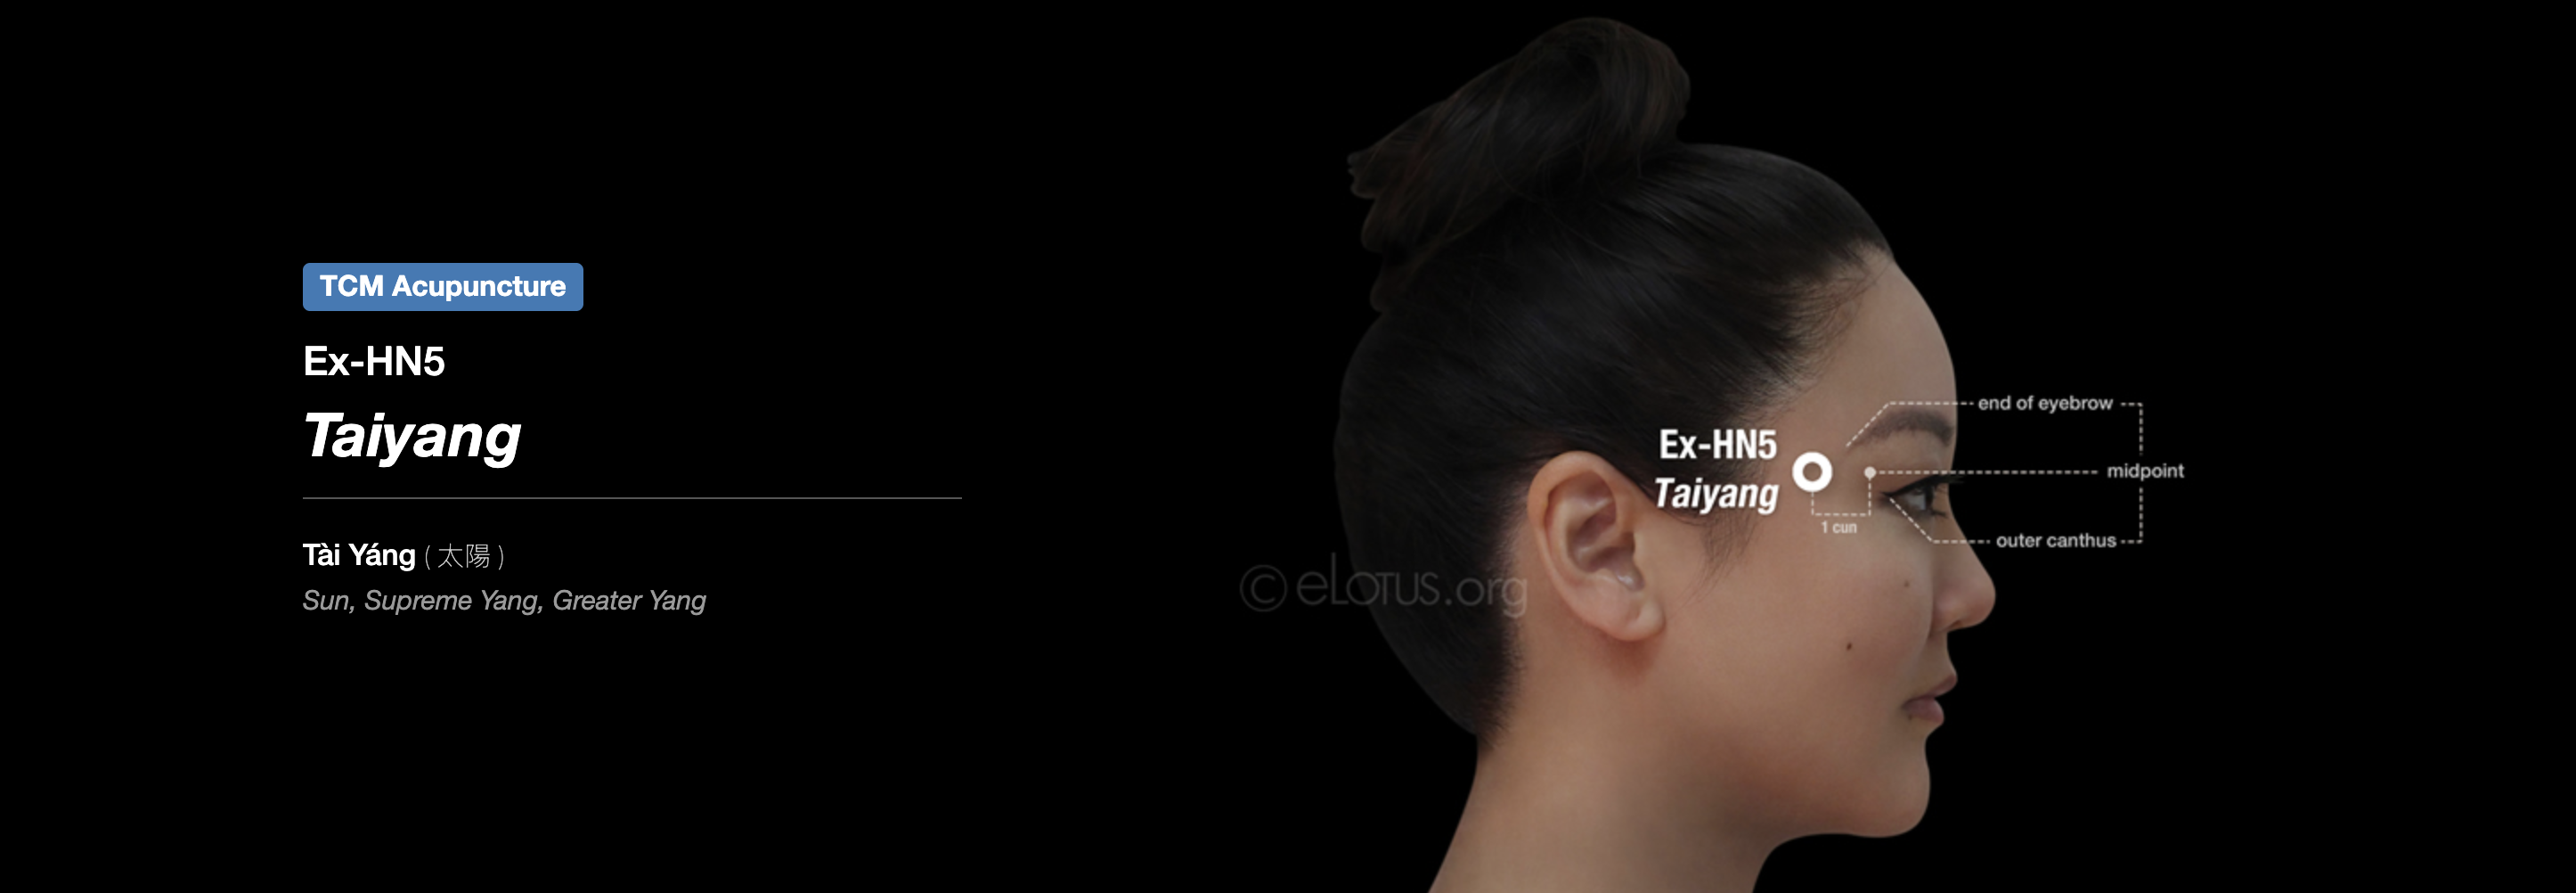
\includegraphics[width=1\linewidth]{images/taiyang-ex-hn5.png}
    \caption{Huyệt thái dương}
    \label{fig:placeholder}
\end{figure}

Thoát vị đĩa đệm hạn chế động tác đẩy đùi.
Vận động khớp gối (vận động) và vận động khớp háng (đẩy đến tận đùi)


- Lưỡi -> chấm -> ứ huyết -> tím (tía chứ không hồng).

% cam du, huyết du, ...

Fenavip - bổ máu - thuốc thái
Dâu - bổ thận bổ máu. Men (đường men rượu, rượu lên men thành giấm, ...)
Dâu sấy - cho người tiểu đường.
Tằm mới có ezim để chuyển hoá lá dâu thành đường, con sâu khác không có ăn chết luôn.

Người nóng chân lạnh -> Tâm thận bất giao -> Giao thái hoà tâm thận -> Làm ấm thận -> Kinh dịch (quả thuỷ hoả quý tế, ...thuỷ hoả kí tuế, hoả thị vị tế, ...), bàn về nhân sinh.


Nhịp tim  nhanh , huyết áp thấp -> thiếu máu.

Ngũ hành âm dương

Hạ đường huyết

\subsubsection{Phương pháp trầm khí tự nhiên}

\begin{figure}[H]
    \centering
    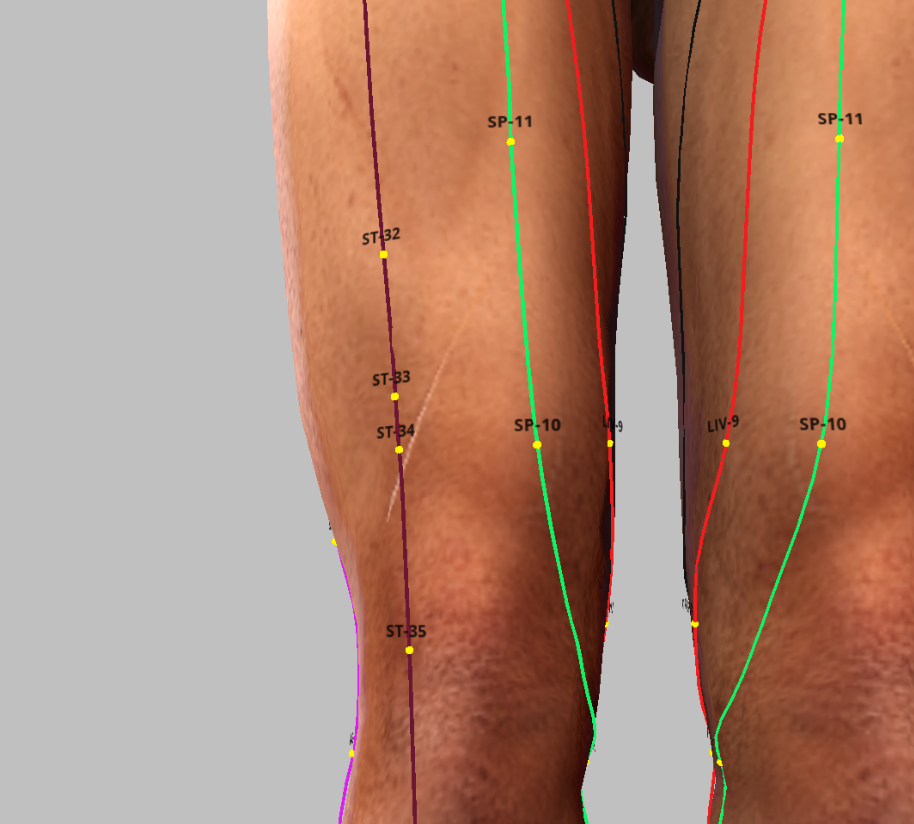
\includegraphics[width=0.25\linewidth]{images/sp10.png}
    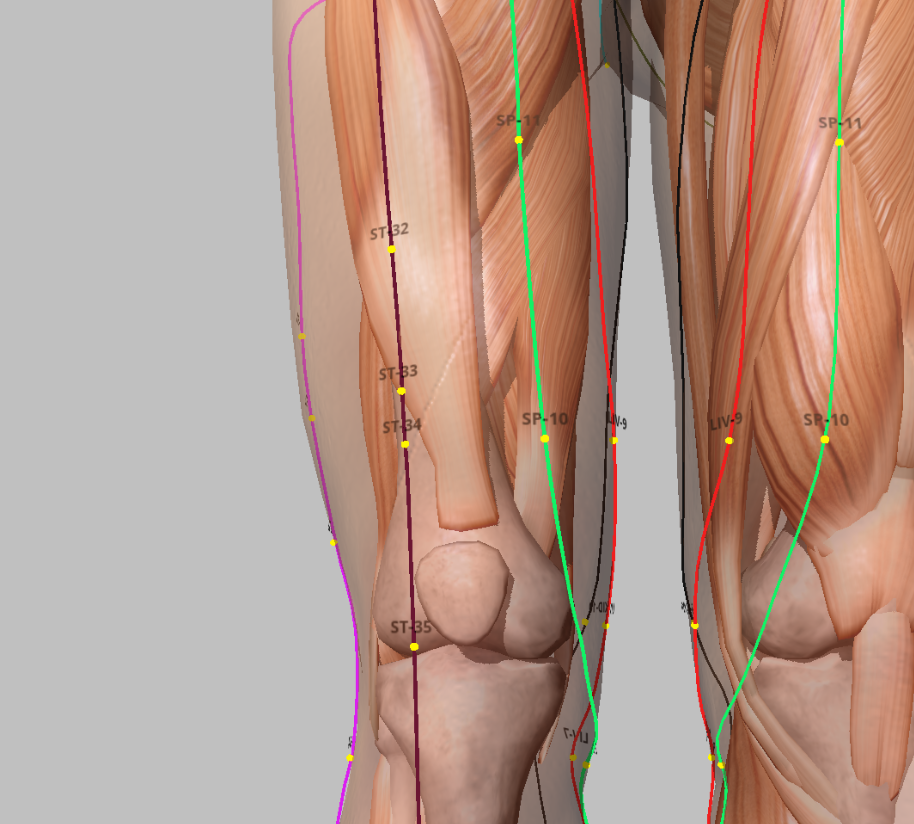
\includegraphics[width=0.25\linewidth]{images/sp10.b.png}
    \caption{SP10, ST34}
    \label{fig:placeholder}
\end{figure}

\subsection{Phương pháp tĩnh khí}
\section{Cơ}

Hệ cơ trong cơ thể con người phụ trách các hoạt động chuyển động, duy trì tư thế và tạo ra nhiệt lượng, được chia thành 3 loại chính:

\subsection{Cơ vân (Cơ xương)}
\begin{itemize}
    \item \textbf{Cấu trúc:} Các sợi cơ dài, có nhiều nhân và xuất hiện các vân ngang sáng tối xen kẽ dưới kính hiển vi.
    \item \textbf{Hoạt động:} Bám vào xương qua hệ thống gân, hoạt động theo ý muốn (chủ động) dưới sự điều khiển của hệ thần kinh trung ương.
    \item \textbf{Chức năng:} Giúp cơ thể thực hiện các cử động như đi lại, cầm nắm, chạy nhảy và duy trì tư thế.
\end{itemize}

\subsection{Cơ trơn}
\begin{itemize}
    \item \textbf{Cấu trúc:} Các tế bào cơ hình thoi, chỉ có một nhân ở trung tâm và không có vân ngang.
    \item \textbf{Hoạt động:} Hoạt động tự động, không theo ý muốn (bất chủ động), chịu sự điều khiển của hệ thần kinh thực vật và hormone.
    \item \textbf{Vị trí \& Chức năng:} Nằm ở thành các cơ quan nội tạng (dạ dày, ruột, bàng quang) và thành mạch máu; giúp co bóp đẩy thức ăn, điều hòa huyết áp và lưu thông khí huyết.
\end{itemize}

\subsection{Cơ tim}
\begin{itemize}
    \item \textbf{Cấu trúc:} Chỉ có ở thành tim. Tế bào cơ tim có vân ngang giống cơ vân nhưng các sợi cơ phân nhánh và nối với nhau qua các đĩa gian bào (intercalated discs).
    \item \textbf{Hoạt động:} Hoạt động tự động, nhịp nhàng và liên tục không nghỉ ngơi, không theo ý muốn.
    \item \textbf{Chức năng:} Co bóp liên tục để bơm máu đi khắp cơ thể qua hệ thống tuần hoàn.
\end{itemize}
Phân loại cơ
- Cơ nhị đầu
- Cơ tam đầu
- Cơ nhị thân (dưới cằm)

Cơ vùng đầu mặt cổ bám vào ra, nguyên uỷ xương, khi co tạo biểu cảm cảm xúc.

Cơ trên móng, cơ dưới móng.

\section{Hệ thần kinh}
Não -> thân -> chi
Hệ thần kinh động vật -> Vận dộng chủ động (Co thì co duỗi thì duỗi)
Hệ thần kinh thực vật -> Ngủ tim vẫn đập.
Đơn vị cấu tạo đơn vị nhỏ nhất là noron thần kinh.

\subsection{Cấu tạo neuron}

Neuron (tế bào thần kinh) là đơn vị cấu tạo và chức năng cơ bản của hệ thần kinh, có nhiệm vụ tiếp nhận, xử lý và truyền dẫn xung thần kinh. Mỗi neuron gồm 3 thành phần chính:

\begin{itemize}
    \item \textbf{Thân neuron (Soma / Cell Body):} 
    \begin{itemize}
        \item Chứa nhân tế bào và các bào quan (như thể Nissl, bộ Golgi, ti thể) đảm nhận chức năng duy trì sự sống và tổng hợp chất dẫn truyền thần kinh.
        \item Là trung tâm trung hòa và xử lý các tín hiệu truyền về.
    \end{itemize}

    \item \textbf{Sợi nhánh (Dendrites):} 
    \begin{itemize}
        \item Là các nhánh ngắn, phân nhánh nhiều như cành cây vươn ra từ thân neuron.
        \item Nhiệm vụ: Tiếp nhận xung thần kinh từ các neuron khác hoặc cơ quan thụ cảm để truyền về thân neuron.
    \end{itemize}

    \item \textbf{Sợi trục (Axon):} 
    \begin{itemize}
        \item Là một sợi dài duy nhất dẫn xung thần kinh đi ra xa thân neuron đến các tế bào đích (neuron khác, cơ hoặc tuyến).
        \item \textit{Bao Myelin:} Bao bọc xung quanh sợi trục (do tế bào Schwann hoặc tế bào sừng ít nhánh tạo thành), giúp cách điện và tăng tốc độ truyền xung thần kinh.
        \item \textit{Eo Ranvier:} Các khoảng hở giữa các bao myelin, giúp xung thần kinh truyền theo kiểu nhảy vọt.
        \item \textit{Cúc synap (Axon terminal):} Phần tận cùng của sợi trục chứa các túi hóa chất trung gian truyền tin (chất dẫn truyền thần kinh).
    \end{itemize}
\end{itemize}

\subsection{Hệ thần kinh trung ương}

Hệ thần kinh trung ương (Central Nervous System - CNS) là trung tâm điều khiển và xử lý thông tin cao nhất của cơ thể, bao gồm não bộ và tủy sống.

\begin{itemize}
    \item \textbf{Não bộ (Brain):} Nằm trong hộp sọ, được bao bọc bởi 3 lớp màng não và dịch não tủy để bảo vệ.
    \begin{itemize}
        \item \textit{Đại não (Cerebrum):} Chiếm thể tích lớn nhất, chia làm hai bán cầu não. Đảm nhận các chức năng nhận thức cao cấp như tư duy, trí nhớ, ngôn ngữ, cảm giác và vận động chủ động.
        \item \textit{Thân não (Brainstem):} Gồm hành não, cầu não và não giữa. Chứa các trung khu điều khiển chức năng sống còn tự động như nhịp tim, hô hấp, huyết áp và phản xạ nuốt.
        \item \textit{Tiểu não (Cerebellum):} Nằm phía sau thân não, có vai trò điều hòa trương lực cơ, giữ thăng bằng và phối hợp các vận động tinh vi.
        \item \textit{Gian não (Diencephalon):} Gồm đồi thị (trạm chuyển tiếp cảm giác) và vùng dưới đồi (điều hòa nội tiết, thân nhiệt, cảm giác đói/khát).
    \end{itemize}

    \item \textbf{Tủy sống (Spinal Cord):} 
    \begin{itemize}
        \item Nằm trong ống sống của cột sống, kéo dài từ hành não xuống đến đốt sống thắt lưng L1-L2.
        \item \textit{Dẫn truyền:} Là đường dẫn truyền tín hiệu thần kinh hai chiều giữa não bộ và các cơ quan ngoại vi (đường cảm giác đi lên và đường vận động đi xuống).
        \item \textit{Phản xạ:} Là trung tâm của các phản xạ tủy không điều kiện (như phản xạ đầu gối, phản xạ rút tay khi chạm vật nóng).
    \end{itemize}
\end{itemize}

\subsection{Thân não và tiểu não}

Thân não và tiểu não đóng vai trò cầu nối quan trọng giữa não bộ với tủy sống, chịu trách nhiệm duy trì các chức năng sống còn và điều hòa vận động.

\subsubsection{Thân não (Brainstem)}

Thân não nằm ở đáy não, nối liền đại não với tủy sống, bao gồm 3 phần chính từ trên xuống dưới:

\begin{itemize}
    \item \textbf{Trung khẩu (Trung não - Midbrain):}
    \begin{itemize}
        \item \textit{Chức năng:} Chứa các trung khu phản xạ thị giác (chuyển động của mắt) và thính giác, tham gia điều hòa vận động và mức độ tỉnh táo.
        \item \textit{Khi tổn thương:} Gây rối loạn vận động mắt (sụp mi, lác, nhìn đôi), mất phản xạ ánh sáng, và các triệu chứng giống bệnh Parkinson do tổn thương chất đen (substantia nigra).
    \end{itemize}

    \item \textbf{Cầu não (Pons):}
    \begin{itemize}
        \item \textit{Chức năng:} Là cầu nối dẫn truyền tín hiệu giữa đại não, tiểu não và tủy sống; tham gia điều hòa nhịp thở và điều khiển các cơ mặt, cảm giác vùng mặt.
        \item \textit{Khi tổn thương:} Gây liệt mặt, mất cảm giác mặt, rối loạn nhịp thở, lác mắt, hoặc nghiêm trọng hơn là hội chứng khóa trong (Locked-in syndrome - bệnh nhân tỉnh táo nhưng liệt toàn thân ngoại trừ cử động mắt).
    \end{itemize}

    \item \textbf{Hành tổng (Hành - Medulla Oblongata):}
    \begin{itemize}
        \item \textit{Chức năng:} Chứa các trung khu sinh mạng cực kỳ quan trọng điều hòa tim mạch, hô hấp (nhịp thở, huyết áp) và các phản xạ bảo vệ (ho, nuốt, nôn, hắt hơi).
        \item \textit{Khi tổn thương:} Dẫn đến nguy cơ tử vong cao do ngừng thở hoặc ngừng tim; gây nuốt khó, sặc, khàn tiếng, tụt huyết áp và mất các phản xạ bảo vệ đường hô hấp.
    \end{itemize}
\end{itemize}

\subsubsection{Tiểu não (Cerebellum)}

Tiểu não nằm ở phía sau thân não, ngay bên dưới thùy chẩm của đại não.

\begin{itemize}
    \item \textbf{Chức năng:}
    \begin{itemize}
        \item Phối hợp và tinh chỉnh các chuyển động tự chủ giúp vận động diễn ra mượt mà, chính xác.
        \item Duy trì thăng bằng và trương lực cơ cho cơ thể.
        \item Lưu trữ các ký ức vận động (như đi xe đạp, đánh máy).
    \end{itemize}

    \item \textbf{Khi tổn thương (Hội chứng tiểu não):}
    \begin{itemize}
        \item \textit{Thất ngôn / Rối loạn thăng bằng:} Dáng đi xiêu vẹo, loạng ạng như người say rượu (Ataxia).
        \item \textit{Mất phối hợp động tác:} Run khi cố tình làm động tác (Intentional tremor), không ước lượng được khoảng cách (Quá tầm - Dysmetria).
        \item \textit{Rối loạn cử động mắt \& Ngôn ngữ:} Giật nhãn cầu (Nystagmus), nói lắp, nói đứt quãng.
        \item \textit{Giảm trương lực cơ:} Cơ nhẽo, phản xạ gân xương giảm.
    \end{itemize}
\end{itemize}

\subsection{Tủy sống}

Tủy sống (Spinal cord) là một phần của hệ thần kinh trung ương, nằm trong ống sống và đóng vai trò cầu nối thần kinh quan trọng giữa não bộ và phần còn lại của cơ thể.

\subsubsection{Cấu tạo giải phẫu}
\begin{itemize}
    \item \textbf{Vị trí:} Kéo dài từ lỗ chẩm của hành não xuống đến ngang mức đốt sống thắt lưng L1--L2.
    \item \textbf{Chất xám (Grey Matter):} Nằm ở bên trong, có hình chữ H (hoặc hình con bướm), chứa thân của các neuron và tế bào thần kinh đệm.
    \begin{itemize}
        \item \textit{Sừng trước (Sừng vận động):} Chứa thân neuron vận động, phát ra các xung thần kinh điều khiển cơ vân.
        \item \textit{Sừng sau (Sừng cảm giác):} Tiếp nhận các tín hiệu cảm giác từ ngoại vi truyền về.
        \item \textit{Sừng bên (Thần kinh thực vật):} Chứa tế bào thần kinh giao cảm (ở đoạn ngực và thắt lưng).
    \end{itemize}
    \item \textbf{Chất trắng (White Matter):} Nằm bao bọc bên ngoài chất xám, gồm các dải/bó sợi thần kinh có bao Myelin đảm nhận nhiệm vụ dẫn truyền tín hiệu.
\end{itemize}

\subsubsection{Chất trắng trong tủy sống và chức năng chi phối}
\begin{itemize}
    \item \textbf{Giải thích chất trắng:} Chất trắng cấu tạo chủ yếu từ các sợi trục thần kinh được bọc bởi \textbf{bao Myelin} (chứa nhiều lipid mang màu trắng đặc trưng). Bao Myelin đóng vai trò cách điện và giúp xung thần kinh truyền đi với tốc độ rất nhanh.
    \item \textbf{Sự chi phối của chất trắng (Các đường dẫn truyền):}
    \begin{itemize}
        \item \textit{Đường cảm giác đi lên (Ascending pathways):} Dẫn truyền tín hiệu cảm giác (đau, nhiệt, tiếp xúc, vị thế khớp) từ cơ thể lên não (ví dụ: Bó gai - đồi thị).
        \item \textit{Đường vận động đi xuống (Descending pathways):} Dẫn truyền lệnh vận động từ não bộ xuống sừng trước tủy sống để chi phối các cơ (ví dụ: Bó tháp / Bó vỏ - gai).
        \item \textit{Bó liên hợp intersegmental:} Kết nối các phân đoạn tủy sống lại với nhau để phối hợp các phản xạ đa phân đoạn.
    \end{itemize}
\end{itemize}

\subsubsection{Chi phối vận động và cảm giác}
\begin{itemize}
    \item Tủy sống phát ra \textbf{31 đôi dây thần kinh tủy} (8 cổ, 12 ngực, 5 thắt lưng, 5 cùng, 1 cúc) chui qua các lỗ liên hợp.
    \item \textbf{Chi phối cảm giác (Dermatome):} Mỗi đôi dây thần kinh tủy đảm nhận cảm giác cho một vùng da xác định trên cơ thể.
    \item \textbf{Chi phối vận động (Myotome):} Chi phối các nhóm cơ tương ứng tại chi trên, thân mình và chi dưới.
\end{itemize}

\subsubsection{Trung tâm của phản xạ không điều kiện}
Tủy sống là trung tâm điều khiển của nhiều **phản xạ không điều kiện** (phản xạ tủy) — là những phản xạ bẩm sinh, tự động, không cần thông qua sự suy nghĩ của vỏ não:
\begin{itemize}
    \item \textbf{Cung phản xạ tủy:} Bao gồm Cơ quan thụ cảm $\rightarrow$ Neuron cảm giác $\rightarrow$ Trung khu tủy sống $\rightarrow$ Neuron vận động $\rightarrow$ Cơ quan đáp ứng.
    \item \textbf{Ví dụ điển hình:}
    \begin{itemize}
        \item \textit{Phản xạ gân xương:} Phản xạ bánh chè (gõ vào gân bánh chè làm duỗi chân).
        \item \textit{Phản xạ bảo vệ:} Phản xạ rút tay/chân khi chạm vào vật nóng hoặc nhọn.
        \item \textit{Phản xạ thực vật:} Điều khiển bài tiết mồ hôi, phản xạ co bóp bàng quang (tiểu tiện) và ruột (đại tiện).
    \end{itemize}
\end{itemize}

\subsection{Hệ thần kinh ngoại biên}

Hệ thần kinh ngoại biên (Peripheral Nervous System - PNS) bao gồm toàn bộ các dây thần kinh và hạch thần kinh nằm ngoài hệ thần kinh trung ương, đóng vai trò kết nối não bộ và tủy sống với các cơ quan trên cơ thể.

\subsubsection{12 đôi dây thần kinh sọ (Cranial Nerves)}

12 đôi dây thần kinh sọ xuất phát từ não bộ (chủ yếu từ thân não), đảm nhận các chức năng cảm giác, vận động và thực vật vùng đầu, mặt, cổ và các cơ quan nội tạng:

\begin{itemize}
    \item \textbf{Dây I (Thần kinh Khứu giác):} Dây cảm giác, đảm nhận chức năng ngửi (khứu giác).
    
    \item \textbf{Dây II (Thần kinh Thị giác):} Dây cảm giác, đảm nhận chức năng nhìn (thị giác). Đây là dây thần kinh sọ duy nhất có thể quan sát trực tiếp đầu tận cùng (đĩa thị) thông qua kỹ thuật \textit{soi đáy mắt}.
    
    \item \textbf{Dây III (Thần kinh Vận nhãn), Dây IV (Thần kinh Bánh xe) \& Dây VI (Thần kinh Vận nhãn ngoài):} 
    \begin{itemize}
        \item Là nhóm dây thần kinh chi phối \textbf{vận động} các cơ vận nhãn.
        \item Trong đó, \textbf{Dây III} đóng vai trò chính trong điều khiển cử động nhãn cầu (co đồng tử, nâng mi mắt, cử động mắt lên/xuống/vào trong).
    \end{itemize}

    \item \textbf{Dây V (Thần kinh Tam thoa / Cốt ba):} 
    \begin{itemize}
        \item Chi phối \textbf{cảm giác vùng mặt} và vận động cơ nhai (hàm).
        \item \textit{Khi tổn thương:} Gây các cơn đau buốt, nhói như điện giật vùng mặt và hàm (đau dây thần kinh số V).
    \end{itemize}

    \item \textbf{Dây VII (Thần kinh Mặt):} 
    \begin{itemize}
        \item Chi phối \textbf{vận động toàn bộ cơ mặt} (tạo biểu cảm) và tiếp nhận \textbf{vị giác 2/3 trước lưỡi}.
        \item \textit{Khi tổn thương:} Dẫn đến liệt mặt ngoại biên (méo miệng, mắt nhắm không kín) và mất/rối loạn vị giác 2/3 trước lưỡi.
    \end{itemize}

    \item \textbf{Dây VIII (Thần kinh Tiền đình - Ốc tai):} Dây cảm giác, đảm nhận chức năng nghe (thính giác) và duy trì sự \textbf{thăng bằng} cho cơ thể.

    \item \textbf{Dây IX (Thần kinh Lưỡi - Hầu), Dây XI (Thần kinh Phụ) \& Dây XII (Thần kinh Hạ thiệt):} Chi phối cảm giác/vị giác 1/3 sau lưỡi, vận động vùng hầu họng, cơ ức đòn chũm, cơ thang và cử động của lưỡi.

    \item \textbf{Dây X (Thần kinh Lang thang / Phế vị):} 
    \begin{itemize}
        \item Là dây \textbf{thần kinh thực vật} (phó giao cảm) lớn nhất cơ thể, đi lang thang phân nhánh rộng khắp đến hầu hết các cơ quan nội tạng ở cổ, ngực và bụng (tim, phổi, dạ dày, ruột...).
        \item Chi phối điều hòa nhịp tim, nhu động tiêu hóa và các phản xạ nội tạng.
    \end{itemize}
\end{itemize}
\subsection{Đám rối thần kinh cánh tay}

Đám rối thần kinh cánh tay (Brachial Plexus) được hợp thành từ ngành trước của các dây thần kinh sống từ **C5 đến T1** (có thể nhận thêm nhánh nhỏ từ C4 hoặc T2). Đám rối này đảm nhận vai trò chi phối toàn bộ vận động và cảm giác cho vùng vai, ngực và chi trên.

\subsubsection{Cấu trúc nguyên ủy và sự liên quan rễ -- ngón tay}

Từ các rễ thần kinh $C5 - T1$, đám rối trải qua các giai đoạn: **Rễ $\rightarrow$ Thân $\rightarrow$ Ngành $\rightarrow$ Bó $\rightarrow$ Các dây thần kinh ngoại biên**. Cảm giác vùng da các ngón tay được chi phối bởi các rễ tương ứng:
\begin{itemize}
    \item \textbf{Rễ C6:} Chi phối cảm giác vùng bờ ngoài cẳng tay, ngón cái (ngón I) và ngón trỏ (ngón II).
    \item \textbf{Rễ C7:} Chi phối cảm giác ngón giữa (ngón III).
    \item \textbf{Rễ C8:} Chi phối cảm giác ngón nhẫn (ngón IV) và ngón út (ngón V).
    \item \textbf{Rễ T1:} Chi phối cảm giác phía bờ trong cẳng tay và cẳng tay dưới.
\end{itemize}

\subsubsection{Các dây thần kinh chính và chi phối vận động -- cảm giác}

\begin{itemize}
    \item \textbf{Thần kinh Nách (Axillary Nerve -- $C5, C6$):}
    \begin{itemize}
        \item \textit{Vận động:} Cơ deltoid (dang cánh tay) và cơ tròn bé.
        \item \textit{Cảm giác:} Cảm giác vùng nách, vai và mặt ngoài phía trên cánh tay.
    \end{itemize}

    \item \textbf{Thần kinh Cơ bì (Musculocutaneous Nerve -- $C5, C6, C7$):}
    \begin{itemize}
        \item \textit{Vận động:} Chi phối nhóm cơ khu cánh tay trước (cơ nhị đầu cánh tay, cơ quạ cánh tay, cơ cánh tay) giúp gấp cẳng tay và ngửa cẳng tay.
        \item \textit{Cảm giác (Thần kinh da cẳng tay ngoài):} Chi phối cảm giác vùng da bờ ngoài cẳng tay.
    \end{itemize}

    \item \textbf{Thần kinh Giữa (Median Nerve -- $C6, C7, C8, T1$):}
    \begin{itemize}
        \item \textit{Vận động:} Hầu hết các cơ gấp cẳng tay, cơ sấp, và các cơ mô cái ở bàn tay (cho phép đối chiếu ngón cái, gấp ngón I, II, III).
        \item \textit{Cảm giác:} Cảm giác mặt lòng bàn tay phía bờ ngoài (ngón cái, ngón trỏ, ngón giữa và $1/2$ ngoài ngón nhẫn) cùng đầu các ngón tương ứng ở mặt lưng.
    \end{itemize}

    \item \textbf{Thần kinh Trụ (Ulnar Nerve -- $C8, T1$):}
    \begin{itemize}
        \item \textit{Vận động:} Các cơ nội tại bàn tay (cơ khép ngón cái, các cơ gian thoa, cơ giun III-IV) và cơ gấp cổ tay trụ.
        \item \textit{Cảm giác:} Chi phối cảm giác bờ trong bàn tay (cả mặt lòng và mặt lưng), ngón út (ngón V) và $1/2$ trong ngón nhẫn (ngón IV).
    \end{itemize}

    \item \textbf{Thần kinh Quay (Radial Nerve -- $C5, C6, C7, C8, T1$):}
    \begin{itemize}
        \item \textit{Vận động:} Chi phối toàn bộ nhóm cơ duỗi ở khu cánh tay sau (cơ tam đầu) và cẳng tay sau (duỗi cổ tay, duỗi các ngón tay và ngửa cẳng tay).
        \item \textit{Cảm giác:} Cảm giác mặt sau cánh tay, cẳng tay và nửa ngoài mặt lưng bàn tay.
    \end{itemize}
\end{itemize}

\subsection{Thần kinh cơ bì và Thần kinh giữa}

\subsubsection{Thần kinh Cơ bì (Musculocutaneous Nerve)}
\begin{itemize}
    \item \textbf{Chi phối vận động:} Chi phối các cơ khu cánh tay trước (cơ nhị đầu cánh tay, cơ quạ cánh tay và cơ cánh tay), đóng vai trò chính giúp \textbf{gấp cẳng tay} và ngửa cẳng tay.
    \item \textbf{Chi phối cảm giác:} Đảm nhận cảm giác mặt ngoài của cẳng tay (thông qua nhánh thần kinh da cẳng tay ngoài).
\end{itemize}

\subsubsection{Thần kinh Giữa (Median Nerve)}
\begin{itemize}
    \item \textbf{Chi phối vận động:}
    \begin{itemize}
        \item Chi phối hầu hết các cơ gấp khu cẳng tay trước và cơ sấp.
        \item Kiểm soát hoạt động của các cơ \textbf{ô mô cái} (cho phép gấp, đối chiếu ngón cái) và các cơ giun I, II.
        \item Tham gia phối hợp vận động vùng cẳng tay, cổ tay (cường tay, gốc tay) và bàn tay.
    \end{itemize}

    \item \textbf{Chi phối cảm giác:}
    \begin{itemize}
        \item Chi phối cảm giác **gan bàn tay** ở phía bờ ngoài.
        \item Chi phối mặt lòng của **ngón 1 (ngón cái)**, **ngón 2 (ngón trỏ)**, ngón 3 (ngón giữa) và nửa ngoài **ngón 4 (ngón áp út)**.
        \item \textit{Lưu ý:} Vùng ô mô út do thần kinh trụ đảm nhận chi phối cảm giác và vận động.
    \end{itemize}

    \item \textbf{Lâm sàng khi bị tổn thương thần kinh giữa:}
    \begin{itemize}
        \item \textbf{Biến dạng bàn tay:} Tình trạng teo cơ vùng ô mô cái khiến bàn tay bị phẳng dẹt, xuất hiện **dấu hiệu bàn tay khỉ** (Monkey hand) hoặc **bàn tay quắp** / bàn tay cầu nguyện khi cố nắm lại.
        \item \textbf{Teo cơ \& Yếu cơ:} Teo cơ ô mô cái và các cơ vùng cẳng tay trước, cơ yếu làm bàn tay có xu hướng bị rũ xuống.
        \item \textbf{Mất khả năng gấp ngón:} **Không gấp được đốt cuối của ngón trỏ (ngón 2) và ngón giữa (ngón 3)** do mất chức năng của cơ gấp sâu các ngón tay.
        \item \textbf{Rối loạn cảm giác:} Mất hoặc giảm cảm giác ở vùng gan bàn tay và các ngón 1, 2, 3 cùng nửa ngoài ngón 4.
    \end{itemize}
\end{itemize}

\subsection{Thần kinh trụ (Ulnar Nerve)}

Thần kinh trụ ($C8 - T1$) là dây thần kinh chính đảm nhận nhiệm vụ điều khiển các vận động tinh vi của bàn tay và chi phối cảm giác bờ trong bàn tay.

\subsubsection{Chi phối vận động và cảm giác}
\begin{itemize}
    \item \textbf{Chi phối vận động tinh vi:}
    \begin{itemize}
        \item Chi phối hầu hết các cơ nội tại của bàn tay, bao gồm: nhóm cơ ô mô út, cơ khép ngón cái, các cơ gian thoa (gan tay và lưng tay) và các cơ giun III, IV.
        \item Đảm nhận các động tác **vận động tinh vi**, khéo léo của các ngón tay như: xòe/khép các ngón tay, kẹp giữ vật giữa các ngón, gảy đàn hoặc viết chữ.
        \item Chi phối cơ gấp cổ tay trụ và nửa trong cơ gấp sâu các ngón tay ở cẳng tay.
    \end{itemize}

    \item \textbf{Chi phối cảm giác:}
    \begin{itemize}
        \item Chi phối toàn bộ cảm giác vùng **ngón 5 (ngón út)** và **nửa trong ngón 4 (ngón áp út)** (cả mặt lòng lẫn mặt lưng).
        \item Chi phối cảm giác vùng bờ trong bàn tay và ô mô út.
    \end{itemize}
\end{itemize}

\subsubsection{Lâm sàng khi bị tổn thương thần kinh trụ}
\begin{itemize}
    \item \textbf{Dấu hiệu Bàn tay vuốt trụ (Vuốt chim / Ulnar Claw):} 
    \begin{itemize}
        \item Do mất chức năng các cơ giun III, IV và cơ gian thoa, dẫn đến hiện tượng **đốt 1 (đốt gần) của ngón 4 và ngón 5 luôn bị duỗi thẳng quá mức** (duỗi khớp bàn - ngón), trong khi đốt 2 và đốt 3 lại bị gấp lại.
    \end{itemize}

    \item \textbf{Teo cơ \& Bàn tay gầy guộc:} 
    \begin{itemize}
        \item Teo rõ rệt vùng cơ ô mô út, teo các cơ gian thoa ở mu bàn tay (đặc biệt là hố gian thoa I giữa ngón cái và ngón trỏ).
        \item Bàn tay bị biến dạng, rãnh xương lộ rõ tạo hình ảnh **bàn tay gầy guộc, gầy còm như vuốt chim**.
    \end{itemize}

    \item \textbf{Mất vận động tinh vi \& Giảm cảm giác:}
    \begin{itemize}
        \item Mất khả năng xòe/khép các ngón tay, khó thực hiện các thao tác đòi hỏi sự khéo léo.
        \item Mất hoặc giảm cảm giác hoàn toàn ở ngón 5 và nửa trong ngón 4.
    \end{itemize}
\end{itemize}

\subsection{Thần kinh quay (Radial Nerve)}

Thần kinh quay ($C5 - T1$) là dây thần kinh lớn nhất xuất phát từ đám rối thần kinh cánh tay, chạy dọc theo rãnh thần kinh quay ở mặt sau xương cánh tay.

\subsubsection{Chi phối vận động và phản xạ}
\begin{itemize}
    \item \textbf{Vị trí \& Chi phối vận động:} 
    \begin{itemize}
        \item Chi phối nhóm cơ khu cánh tay sau (cơ tam đầu cánh tay) giúp **duỗi cẳng tay**.
        \item Chi phối toàn bộ nhóm cơ khu cẳng tay sau và ngoài, giúp **duỗi cổ tay, duỗi các ngón tay và ngửa cẳng tay**.
    \end{itemize}
    \item \textbf{Phản xạ:} Đảm nhận cung phản xạ gân cơ tam đầu (C7).
    \item \textbf{Chi phối cảm giác:} Chi phối cảm giác mặt sau cánh tay, cẳng tay và nửa ngoài mặt lưng bàn tay (ngón 1, 2, 3 và nửa ngoài ngón 4).
\end{itemize}

\subsubsection{Lâm sàng khi bị tổn thương thần kinh quay}
\begin{itemize}
    \item \textbf{Nguyên nhân thường gặp:} Rất hay gặp trong **gãy $1/3$ giữa hoặc $1/3$ dưới xương cánh tay** (do dây thần kinh đi sát vào rãnh xoắn của xương) hoặc do chèn ép kéo dài (liệt thứ bảy tuần / Saturday night palsy).
    \item \textbf{Dấu hiệu Bàn tay rủ (Hand drop / Bàn tay cổ cò):}
    \begin{itemize}
        \item Bệnh nhân **không thể duỗi cổ tay và các ngón tay**.
        \item Cổ tay và bàn tay luôn ở trạng thái **gấp rủ xuống** liên tục.
    \end{itemize}
    \item \textbf{Mất phản xạ:} **Mất phản xạ gân cơ tam đầu** và giảm/mất phản xạ gân cơ trâm quay.
    \item \textbf{Mất khả năng ngửa cẳng tay} khi cẳng tay đang duỗi và giảm lực kẹp của bàn tay.
    \item \textbf{Rối loạn cảm giác:} Tê bì hoặc mất cảm giác vùng kẽ ngón tay I - II ở mặt lưng bàn tay (hố xẩu giải phẫu).
\end{itemize}

\subsection{Đám rối thần kinh thắt lưng -- cùng}

Đám rối thần kinh thắt lưng -- cùng (Lumbosacral Plexus) được hợp thành từ ngành trước của các dây thần kinh sống từ **L1 đến S4**, chi phối vận động và cảm giác cho chi dưới, vùng chậu và tầng sinh môn. Trong đó, thần kinh tọa (thần kinh hông to - $L4, L5, S1, S2, S3$) là dây thần kinh lớn nhất và dài nhất trong cơ thể.

\subsubsection{Chi phối vận động và cảm giác}
\begin{itemize}
    \item \textbf{Vùng chi phối vận động:}
    \begin{itemize}
        \item Chi phối toàn bộ nhóm cơ khu **đùi sau** (nhóm cơ gân kheo: cơ bán gân, cơ bán màng, cơ nhị đầu đùi) giúp gấp cẳng chân.
        \item Chi phối toàn bộ **vùng dưới gối** (cẳng chân và bàn tay/bàn chân) thông qua hai nhánh tận là thần kinh chày và thần kinh mác chung.
    \end{itemize}

    \item \textbf{Vùng chi phối cảm giác:} Đảm nhận cảm giác mặt sau đùi, toàn bộ vùng cẳng chân và bàn chân (trừ mặt trong cẳng chân do thần kinh hiển chi phối).
\end{itemize}

\subsubsection{Biểu hiện lâm sàng tổn thương và chèn ép (Đau thần kinh tọa)}
\begin{itemize}
    \item \textbf{Hướng lan đặc trưng:} Cơn đau thường bắt đầu từ vùng thắt lưng hoặc mông, **hay lan xuống đùi** (mặt sau hoặc mặt ngoài) và tiếp tục lan xuống dưới gối, cẳng chân rồi đến tận bàn chân, ngón chân.
    \item \textbf{Triệu chứng cơ năng:}
    \begin{itemize}
        \item **Tê nhức, châm chích:** Cảm giác tê bì, rát bỏng hoặc nhức nhối kéo dài dọc theo đường đi của dây thần kinh.
        \item **Yếu cơ \& Rối loạn vận động:** Khi tổn thương nặng gây yếu các cơ vùng cẳng chân, dẫn đến khó khăn khi đi lại (khó đi bằng mũi chân hoặc gót chân), có thể gây bàn tay/bàn chân rũ (Drop foot).
    \end{itemize}
    \item \textbf{Nguyên nhân thường gặp:} Thoát vị đĩa đệm cột sống thắt lưng (đặc biệt tầng L4-L5 hoặc L5-S1), gai cột sống, hẹp ống sống hoặc hội chứng cơ hình lê (Piriformis syndrome).
\end{itemize}

\subsection{Thần kinh ngồi (Thần kinh tọa)}

Thần kinh ngồi (Sciatic Nerve - $L4, L5, S1, S2, S3$) là dây thần kinh lớn nhất và dài nhất trong cơ thể, xuất phát từ đám rối thần kinh thắt lưng -- cùng.

\subsubsection{Hội chứng đau thần kinh tọa}
\begin{itemize}
    \item \textbf{Đặc điểm cơn đau:} Đau lan dọc theo đường đi của dây thần kinh ngồi, khởi phát từ vùng **thắt lưng**, lan qua **mông**, dọc xuống mặt sau/mặt ngoài đùi, cẳng chân và tận cùng ở bàn chân.
    \item \textbf{Tính chất đau:} Đau nhức nhối, châm chích, có thể kèm theo cảm giác tê bì, rát bỏng hoặc yếu cơ chi dưới.
\end{itemize}

\subsubsection{Chi phối cảm giác và vận động theo từng rễ thần kinh}
Hướng lan của triệu chứng đau và tê chịu sự chi phối cụ thể theo các rễ thần kinh cấu thành:

\begin{itemize}
    \item \textbf{Rễ L5 (Nhánh trước -- mặt ngoài):}
    \begin{itemize}
        \item \textit{Đường lan cảm giác:} Lan từ thắt lưng $\rightarrow$ mặt ngoài mông $\rightarrow$ mặt ngoài đùi $\rightarrow$ mặt trước ngoài cẳng chân $\rightarrow$ mu bàn chân và tận cùng ở **ngón chân cái (ngón I)**.
        \item \textit{Vận động:} Chi phối các cơ gấp mặt lưng cổ tay/bàn chân (cơ cẳng chân trước) $\rightarrow$ tổn thương gây khó khăn khi đi bằng gót chân.
    \end{itemize}

    \item \textbf{Rễ S1 (Mặt sau):}
    \begin{itemize}
        \item \textit{Đường lan cảm giác:} Lan từ thắt lưng $\rightarrow$ đằng sau mông $\rightarrow$ **toàn bộ mặt sau đùi** $\rightarrow$ mặt sau cẳng chân (bắp chân) $\rightarrow$ gót chân, lòng bàn chân và tận cùng ở **ngón út (ngón V)**.
        \item \textit{Vận động:} Chi phối các cơ gấp mặt lòng bàn chân (cơ tam đầu cẳng chân) $\rightarrow$ tổn thương gây khó khăn khi đi bằng mũi chân và làm giảm/mất phản xạ gân gót (gân Achilles).
    \end{itemize}
\end{itemize}

\subsubsection{Nguyên nhân lâm sàng thường gặp}
\begin{itemize}
    \item **Thoát vị đĩa đệm cột sống thắt lưng:** Là nguyên nhân phổ biến nhất (đặc biệt tại vị trí L4--L5 gây chèn ép rễ L5, hoặc L5--S1 gây chèn ép rễ S1).
    \item **Gai cột sống / Hẹp ống sống:** Chèn ép các rễ thần kinh tại vị trí chui ra khỏi lỗ liên hợp.
    \item **Hội chứng cơ hình lê (Piriformis syndrome):** Cơ hình lê ở vùng mông bị co thắt hoặc viêm gây chèn ép dây thần kinh ngồi.
\end{itemize}

\section{Sinh lý hệ thần kinh và Cung phản xạ}

Hệ thần kinh điều khiển, điều hòa và phối hợp mọi hoạt động của các cơ quan trong cơ thể thông qua cơ chế phản xạ.

\subsection{Cung phản xạ thần kinh}

Cung phản xạ là cơ sở thần kinh của mọi phản xạ, gồm 5 thành phần chính hoạt động theo một chu trình khép kín:

\begin{enumerate}
    \item \textbf{Cơ quan thụ cảm (Receptors):} Tiếp nhận các kích thích từ môi trường ngoài hoặc bên trong cơ thể (như nhiệt độ, áp lực, đau đớn, hóa chất).
    \item \textbf{Đường cảm giác (Đường hướng tâm):} Truyền tín hiệu thần kinh từ cơ quan thụ cảm về hệ thần kinh trung ương (tủy sống hoặc não bộ).
    \item \textbf{Trung khu thần kinh (Trung ương phân tích \& chỉ huy):} Não bộ hoặc tủy sống tiếp nhận, phân tích, xử lý thông tin và đưa ra đáp ứng phù hợp.
    \item \textbf{Đường vận động (Đường ly tâm):} Truyền lệnh điều khiển từ trung khu thần kinh đến cơ quan đáp ứng.
    \item \textbf{Cơ quan đáp ứng (Effector):} Các cơ (co hoặc giãn) hoặc các tuyến (tăng hoặc giảm tiết).
\end{enumerate}

\subsection{Sự truyền dẫn và xử lý thông tin}

Quá trình phản xạ diễn ra theo hai cấp độ:
\begin{itemize}
    \item \textbf{Phản xạ tủy (Cấp thấp):} Tín hiệu truyền về tủy sống và phát lệnh đáp ứng ngay tức thì mà chưa cần lên não (như phản xạ rút tay khi bị bỏng).
    \item \textbf{Truyền về não bộ (Cấp cao):} Các đường dẫn truyền cảm giác (bó gai - đồi thị) đưa tín hiệu lên vỏ não để phân tích chi tiết, ghi nhớ và đưa ra đáp ứng vận động hoặc hành vi tinh vi hơn.
\end{itemize}

\subsection{Ứng dụng trong bấm huyệt và điều hòa nội tạng}

Bấm huyệt tác động trực tiếp lên các thụ thể thần kinh ở da và cơ, khởi động cung phản xạ thần kinh - thực vật để điều chỉnh chức năng các cơ quan bên trong:

\begin{itemize}
    \item \textbf{Giảm đau dạ dày:} Bấm các huyệt như \textit{Túc tam lý (ST36)}, \textit{Trung quản (CV12)} truyền tín hiệu thần kinh về tủy sống, kích thích giải phóng các chất giảm đau nội sinh (endorphin) và làm giảm co bóp cơ trơn dạ dày, giúp làm dịu cơn đau tức thì.
    \item \textbf{Cải thiện đầy bụng, khó tiêu:} Tác động lực vào huyệt giúp kích thích hệ thần kinh phó giao cảm (dây thần kinh lang thang - dây X), tăng cường nhu động ruột và đẩy nhanh quá trình tiêu hóa thức ăn.
    \item \textbf{Điều hòa hoạt động của các tuyến:} Cung phản xạ thần kinh - thể dịch giúp tác động lên các tuyến nội tiết và ngoại tiết:
    \begin{itemize}
        \item \textbf{Tăng tiết:} Kích thích các tuyến tiêu hóa (tuyến vị, tuyến tụy) tăng tiết enzym khi tiêu hóa kém.
        \item \textbf{Giảm tiết:} Úc chế, làm giảm tiết acid dịch vị $HCl$ ở dạ dày đối với người bị viêm loét dạ dày - tá tràng.
    \end{itemize}
\end{itemize}

\section{Hệ thần kinh tự chủ và Hoạt động thần kinh cao cấp}

\subsection{Hệ thần kinh tự chủ (Hệ thần kinh thực vật)}

Hệ thần kinh tự chủ điều khiển các hoạt động tự động của các cơ quan nội tạng (tim, phổi, dạ dày, mạch máu...), được chia thành hai hệ thống hoạt động đối kháng và hỗ trợ lẫn nhau:

\begin{itemize}
    \item \textbf{Hệ thần kinh giao cảm (Sympathetic System):}
    \begin{itemize}
        \item \textit{Kích hoạt:} Hoạt động mạnh khi cơ thể gặp trạng thái căng thẳng (stress), sợ hãi, nguy hiểm hoặc vận động thể lực cao (phản ứng "chiến hay biến" - Fight or Flight).
        \item \textit{Biểu hiện:} Làm tăng nhịp tim, tăng huyết áp ("tăng xống"), giãn phế quản, giãn đồng tử, tăng đường huyết và tạm thời ức chế các hoạt động tiêu hóa để dồn năng lượng cho cơ bắp và não bộ.
    \end{itemize}

    \item \textbf{Hệ thần kinh đối giao cảm / Phó giao cảm (Parasympathetic System):}
    \begin{itemize}
        \item \textit{Kích hoạt:} Hoạt động chủ yếu khi cơ thể ở trạng thái nghỉ ngơi, thư giãn, bình yên (trạng thái "nghỉ ngơi và tiêu hóa" - Rest and Digest).
        \item \textit{Biểu hiện:} Làm chậm nhịp tim, hạ huyết áp, co đồng tử, kích thích nhu động ruột, tăng tiết dịch tiêu hóa và tích lũy năng lượng cho cơ thể.
    \end{itemize}
\end{itemize}

\subsection{Hoạt động thần kinh cao cấp}

Hoạt động thần kinh cao cấp là sự phối hợp phức tạp giữa vỏ đại não và các trung khu dưới vỏ, giúp cơ thể thích ứng linh hoạt với môi trường thông qua hai loại phản xạ:

\begin{itemize}
    \item \textbf{Phản xạ không điều kiện:}
    \begin{itemize}
        \item Là những phản xạ bẩm sinh, sinh ra đã có, mang tính chất loài và di truyền.
        \item Trung khu nằm ở các phần dưới vỏ não (tủy sống, thân não).
        \item \textit{Ví dụ:} Co đồng tử khi gặp ánh sáng mạnh, rút tay lại khi chạm vào vật nóng, phản xạ hắt hơi.
    \end{itemize}

    \item \textbf{Phản xạ có điều kiện:}
    \begin{itemize}
        \item Là những phản xạ được hình thành trong đời sống qua quá trình học tập, rèn luyện và kinh nghiệm cá nhân.
        \item Bắt buộc phải có sự tham gia điều khiển của **vỏ đại não**; dễ mất đi nếu không được củng cố thường xuyên.
        \item \textit{Ví dụ:} Dừng xe khi thấy đèn đỏ, tiết nước bọt khi nghe nhắc đến món ăn chua ưa thích.
    \end{itemize}
\end{itemize}

\subsection{Chăm sóc và vệ sinh hệ thần kinh}

Để duy trì hiệu suất làm việc bền bỉ, phòng ngừa suy nhược thần kinh và nâng cao chất lượng cuộc sống, cần thực hiện tốt các biện pháp vệ sinh hệ thần kinh:

\begin{itemize}
    \item \textbf{Đảm bảo giấc ngủ chất lượng:} Ngủ đủ giấc từ **7--8 tiếng mỗi ngày** giúp tế bào thần kinh khôi phục năng lượng, loại bỏ các chất độc hại tích tụ trong não bộ và củng cố trí nhớ.
    \item \textbf{Tránh các chất kích thích:} Hạn chế hoặc loại bỏ rượu, bia, thuốc lá, cà phê quá độ và các chất gây nghiện làm căng thẳng hoặc suy thoái tế bào thần kinh.
    \item \textbf{Dinh dưỡng hợp lý:} Duy trì chế độ ăn giàu chất dinh dưỡng cho não bộ:
    \begin{itemize}
        \item \textit{Omega-3:} Có trong cá hồi, hạt óc chó... giúp cấu tạo màng tế bào thần kinh.
        \item \textit{Vitamin nhóm B (B1, B6, B12):} Giúp bảo vệ bao myelin và hỗ trợ dẫn truyền thần kinh.
    \end{itemize}
    \item \textbf{Luyện tập trí tuệ \& Vận động thể chất:}
    \begin{itemize}
        \item \textit{Tư duy thường xuyên:} Đọc sách, học tập, giải đố giúp duy trì tính linh hoạt của các kết nối synap.
        \item \textit{Tập thể dục đều đặn:} Tăng cường tuần hoàn máu não, kích thích sản sinh các hormone hạnh phúc (endorphin).
    \end{itemize}
\end{itemize}


\section{Tuyến nội tiết và Tuyến ngoại tiết}

Căn cứ vào cấu tạo giải phẫu và phương thức vận chuyển sản phẩm tiết, các tuyến trong cơ thể được chia làm hai loại chính: tuyến ngoại tiết và tuyến nội tiết.

\subsection{So sánh Tuyến ngoại tiết và Tuyến nội tiết}

\begin{itemize}
    \item \textbf{Tuyến ngoại tiết (Exocrine Glands):}
    \begin{itemize}
        \item \textit{Cấu trúc:} **Có ống dẫn** riêng biệt.
        \item \textit{Vị trí tác động:} Đưa sản phẩm tiết trực tiếp đến ngay vị trí gần nơi sản xuất (bề mặt da hoặc lòng các cơ quan rỗng).
        \item \textit{Sản phẩm tiết:} Tiết ra các chất không phải hormone như **mồ hôi, nước bọt, sữa, dịch vị, chất nhờn**.
    \end{itemize}

    \item \textbf{Tuyến nội tiết (Endocrine Glands):}
    \begin{itemize}
        \item \textit{Cấu trúc:} **Không có ống dẫn**.
        \item \textit{Vị trí tác động:} Sản phẩm tiết được ngấm thẳng vào mao mạch và vận chuyển theo dòng máu đến các cơ quan/tế bào ở xa nơi sản xuất.
        \item \textit{Sản phẩm tiết:} Tiết ra các chất hóa học đặc hiệu gọi là **Hormone**.
    \end{itemize}
\end{itemize}

\subsection{Đặc tính sinh lý và Cơ chế tác động của Hormone}

Hormone là những chất hóa học đóng vai trò truyền tin sinh học trong cơ thể với các đặc tính nổi bật:

\begin{itemize}
    \item \textbf{Nồng độ thấp -- Hiệu quả cao:} Hormone được tiết vào máu với lượng cực kỳ nhỏ (nồng độ rất thấp), nhưng có tính hoạt sinh sinh học rất cao, đủ để gây ra những biến đổi lớn về chuyển hóa và chức năng của cơ thể.
    \item \textbf{Tính đặc hiệu (Chỉ tác động lên tế bào đích):} Hormone lưu thông khắp cơ thể qua dòng máu nhưng chỉ gắn vào và tác động lên **tế bào đích** (Target cell) — nơi có các thụ thể (receptor) tiếp nhận đặc hiệu tương ứng.
    \item \textbf{Thời gian tồn tại và chu kỳ bán hủy (Half-life) đa dạng:}
    \begin{itemize}
        \item Thời gian tồn tại của các hormone rất khác nhau tùy thuộc vào bản chất hóa học và vai trò sinh lý.
        \item Một số hormone như \textbf{Adrenaline (Epinephrine)} có thời gian bán hủy rất ngắn (chỉ vài giây đến vài phút): được sinh ra tức thì khi gặp nguy hiểm và tiêu biến nhanh chóng sau đó.
        \item Ngược lại, các hormone steroid (như Estrogen, Cortisol) hay hormone tuyến giáp ($T_3, T_4$) có thể tồn tại và phát huy tác dụng kéo dài vài giờ đến nhiều ngày.
    \end{itemize}
\end{itemize}

\section{Các tuyến nội tiết chính}

\subsection{Vùng dưới đồi (Hypothalamus)}
\begin{itemize}
    \item \textbf{Vị trí:} Nằm ở sàn não thất ba, ngay phía trên thân não và bên dưới đồi thị; là trung tâm kết nối giữa hệ thần kinh và hệ nội tiết.
    \item \textbf{Chức năng điều hòa sinh tồn:} Điều khiển các hoạt động sinh tồn cơ bản của cơ thể như cảm giác **đói/no**, nhịp sinh học (**buồn ngủ/tỉnh táo**), điều hòa **thân nhiệt (nóng/lạnh)**, cảm giác khát và hành vi cảm xúc.
    \item \textbf{Chức năng nội tiết:} Tổng hợp và tiết các **hormone giải phóng (RH)** và **hormone ức chế (IH)** để điều khiển trực tiếp hoạt động tổng hợp, giải phóng hormone của thùy trước tuyến yên.
\end{itemize}

\subsection{Tuyến yên (Pituitary Gland / Hypophysis)}
\begin{itemize}
    \item \textbf{Vị trí:} Nằm ở hố yên của xương bướm, ở đáy não, được nối liền với vùng dưới đồi qua cuống tuyến yên.
    \item \textbf{Cấu trúc giải phẫu:} Được chia thành hai thùy chính:
    \begin{itemize}
        \item \textbf{Thùy trước (Thùy tuyến):} Chiếm khoảng **75\% khối lượng** tuyến yên, chứa các tế bào tuyến chịu sự điều khiển của các hormone từ vùng dưới đồi.
        \item \textbf{Thùy sau (Thùy thần kinh):} Bản chất là mút tận cùng của các sợi thần kinh xuất phát từ vùng dưới đồi, đóng vai trò dự trữ và giải phóng hormone.
    \end{itemize}
\end{itemize}

\subsubsection{Các Hormone thùy trước tuyến yên}
\begin{itemize}
    \item \textbf{GH (Growth Hormone):} Hormone tăng trưởng, kích thích sự phát triển chiều cao, khối lượng cơ thể, xương và phát triển phân chia tế bào.
    \item \textbf{Gonadotropins (FSH \& LH):} Hormone hướng sinh dục, điều khiển hoạt động chức năng của **buồng trứng** (phát triển nang trứng, tiết Estrogen/Progesterone) và **tinh hoàn** (sản sinh tinh trùng, tiết Testosterone).
    \item \textbf{Prolactin (PRL):} Hormone cấu trúc protein có chức năng kích thích tuyến vú phát triển và **sản xuất sữa** ở phụ nữ sau sinh.
    \item \textbf{MSH (Melanocyte-Stimulating Hormone):} Hormone kích thích tế bào hắc tố, đóng vai trò điều hòa tổng hợp Melanin, ảnh hưởng đến **sự thay đổi màu sắc da**.
    \item \textit{Các hormone khác:} TSH (kích thích tuyến giáp), ACTH (kích thích vỏ thượng thận).
\end{itemize}

\subsubsection{Các Hormone thùy sau tuyến yên}
Thùy sau không tự sản xuất hormone mà dự trữ và giải phóng hai hormone do vùng dưới đồi tổng hợp:
\begin{itemize}
    \item \textbf{ADH (Vasopressin - Hormone chống bài niệu):}
    \begin{itemize}
        \item \textit{Chức năng:} Tăng cường **tái hấp thu nước ở ống thận** về máu, làm giảm thể tích nước tiểu. Qua đó điều hòa thể tích máu và **điều hòa huyết áp**.
        \item \textit{Khi bị rối loạn:} Thiếu hụt ADH dẫn đến bệnh đái tháo nhạt (đi tiểu nhiều, mất nước nghiêm trọng), cơ thể **không thể điều hòa được huyết áp** gây tụt huyết áp.
    \end{itemize}

    \item \textbf{Oxytocin:}
    \begin{itemize}
        \item Kích thích **co bóp cơ trơn tử cung** mạnh mẽ trong quá trình chuyển dạ sinh con.
        \item Kích thích co bóp các tế bào biểu mô cơ quanh nang tuyến vú, giúp **bài tiết (tống) sữa** ra ngoài khi trẻ bú.
    \end{itemize}
\end{itemize}


\section{Tuyến giáp và Tuyến cận giáp}

\subsection{Tuyến giáp (Thyroid Gland)}

\subsubsection{Vị trí, cấu trúc và đặc điểm giải phẫu}
\begin{itemize}
    \item \textbf{Vị trí \& Cấu trúc:} Nằm ở phía trước cổ, ngay bên dưới thanh quản và phía trước khí quản. Cấu trúc gồm **2 thùy** (thùy phải và thùy trái) được nối với nhau qua một eo tuyến giáp.
    \item \textbf{Đặc điểm nổi bật:} Là tuyến nội tiết **lớn nhất trong cơ thể** và được **cung cấp lượng máu rất phong phú** (khoảng $4 - 6\text{ ml/phút/g}$ mô tuyến).
\end{itemize}

\subsubsection{Các Hormone tuyến giáp và Chức năng}
\begin{itemize}
    \item \textbf{Hormone $T_3$ (Triiodothyronine) và $T_4$ (Thyroxine):}
    \begin{itemize}
        \item \textit{Thành phần cấu tạo:} Được tổng hợp từ axit amin \textbf{Tyrosine và Iot}.
        \item \textit{Chức năng chính:} Điều hòa chuyển hóa cơ bản của toàn bộ cơ thể, kích thích tăng trưởng tế bào và phát triển hệ thần kinh.
        \item \textit{Tác động lên tim mạch:} **Làm tăng nhịp tim**, tăng sức co bóp cơ tim và tăng huyết áp tâm thu.
        \item \textit{Vai trò của Iot:} Thiếu iot làm tuyến giáp không tổng hợp đủ $T_3, T_4$, dẫn đến phản ứng bù trừ kích thích tuyến giáp phì đại, gây ra **bệnh bướu cổ đơn thuần (bướu cổ do thiếu iot)**.
    \end{itemize}

    \item \textbf{Hormone Calcitonin:} Do các tế bào cận nang của tuyến giáp tiết ra, có vai trò **làm giảm nồng độ $Ca^{2+}$ trong máu** (bằng cách thúc đẩy đưa $Ca^{2+}$ từ máu tích tụ vào xương và tăng bài tiết $Ca^{2+}$ qua thận).
\end{itemize}

\subsubsection{Rối loạn chức năng tuyến giáp (Lâm sàng)}
\begin{itemize}
    \item \textbf{Suy tuyến giáp (Hypothyroidism):} Chuyển hóa cơ bản giảm $\rightarrow$ Bệnh nhân **thường xuyên sợ lạnh, tăng cân/béo phì**, mệt mỏi, nhịp tim chậm, da khô.
    \item \textbf{Cường tuyến giáp (Hyperthyroidism - ví dụ: Bệnh Basedow):} Chuyển hóa cơ bản tăng cao $\rightarrow$ Bệnh nhân **sợ nóng, gầy sút cân nhanh**, nhịp tim nhanh, hồi hộp đánh trống ngực, mắt lồi, hay lo âu.
\end{itemize}

\subsection{Tuyến cận giáp (Parathyroid Glands)}

\subsubsection{Vị trí và cấu trúc}
Gồm 4 tuyến nhỏ kích thước bằng hạt đậu, nằm vùi ở **mặt sau của thùy tuyến giáp** (2 tuyến trên và 2 tuyến dưới).

\subsubsection{Hormone PTH và Điều hòa Canxi máu}
\begin{itemize}
    \item Tuyến cận giáp tiết ra **Hormone Parathyroid (PTH)** — hormone đóng vai trò quyết định trong việc **làm tăng nồng độ $Ca^{2+}$ trong máu**.
    \item \textbf{Cơ chế rút Canxi đổ vào máu:} Khi nồng độ $Ca^{2+}$ trong máu bị giảm (hạ canxi máu), tuyến cận giáp lập tức tăng tiết PTH. PTH sẽ:
    \begin{itemize}
        \item Tác động lên xương: Kích thích hủy xương, **rút $Ca^{2+}$ từ màng xương và chất nền xương đổ vào máu**.
        \item Tác động lên thận và ruột: Tăng tái hấp thu $Ca^{2+}$ ở ống thận và tăng hấp thu $Ca^{2+}$ tại ruột (thông qua hoạt hóa Vitamin D).
    \end{itemize}
    \item \textbf{Ý nghĩa sinh lý:} Khi $Ca^{2+}$ máu tăng trở lại mức sinh lý, sự tiết PTH sẽ bị chế ngự (Feedback âm). Việc duy trì $Ca^{2+}$ máu ổn định có ý nghĩa đặc biệt quan trọng giúp **duy trì tính co bóp bình thường của cơ tim** và sự dẫn truyền xung thần kinh - cơ.
\end{itemize}

\section{Tuyến thượng thận (Adrenal Glands)}

Tuyến thượng thận gồm hai tuyến nhỏ nằm ngay phía trên đỉnh của hai quả thận. Tuyến đóng vai trò sinh tồn trong việc điều hòa cân bằng muối -- nước, duy trì huyết áp và giúp cơ thể ứng phó với các trạng thái căng thẳng (stress).

\subsection{Cấu trúc giải phẫu và Sự phân chia chức năng}

Về mặt giải phẫu và sinh lý, tuyến thượng thận được chia thành hai phần riêng biệt có nguồn gốc và chức năng hoàn toàn độc lập:
\begin{itemize}
    \item \textbf{Vỏ thượng thận (Adrenal Cortex):} Chiếm phần lớn khối lượng bên ngoài của tuyến, sản xuất các hormone steroid sinh tồn.
    \item \textbf{Tủy thượng thận (Adrenal Medulla):} Nằm ở trung tâm của tuyến, bản chất là một phần của hệ thần kinh giao cảm biệt hóa, chịu sự kích thích trực tiếp từ hệ thần kinh.
\end{itemize}

\subsection{Vỏ thượng thận (Adrenal Cortex) và các Hormone tiêu biểu}

Vỏ thượng thận tiết ra các hormone steroid quan trọng, nổi bật nhất là hai nhóm hormone:

\begin{itemize}
    \item \textbf{Mineralocorticoid (Hormone tiêu biểu nhất: Aldosterone):}
    \begin{itemize}
        \item \textit{Chức năng:} **Cân bằng điện giải (muối -- nước)** bằng cách tăng cường tái hấp thu $Na^+$ và nước ở ống thận, đồng thời bài tiết $K^+$ ra nước tiểu ($\rightarrow$ **hạ $K^+$ máu**).
        \item \textit{Vai trò sinh lý:} **Duy trì thể tích máu và điều hòa huyết áp** ổn định cho cơ thể.
    \end{itemize}

    \item \textbf{Glucocorticoid (Hormone tiêu biểu nhất: Cortisol):}
    \begin{itemize}
        \item \textit{Chống căng thẳng (Stress):} Giúp cơ thể thích nghi và chịu đựng các trạng thái căng thẳng về thể xác lẫn tinh thần (chấn thương, phẫu thuật, nhiễm trùng, áp lực tâm lý).
        \item \textit{Chuyển hóa năng lượng:} **Tăng đường huyết** (thúc đẩy tân tạo glucose từ protein và lipid) để cung cấp năng lượng tức thì cho não và cơ bắp.
        \item \textit{Tác dụng dược lý:} Có đặc tính **chống viêm và chống dị ứng** mạnh mẽ, làm giảm các phản ứng miễn dịch quá mức của cơ thể.
    \end{itemize}

    \item \textbf{Androgen (Hormone sinh dục nam):} Tiết ra một lượng nhỏ hỗ trợ phát triển các đặc tính sinh dục phụ thứ phát.
\end{itemize}

\subsection{Tủy thượng thận (Adrenal Medulla)}

\begin{itemize}
    \item \textbf{Các chất tiết ra từ trung tâm tủy thượng thận:} Tiết ra nhóm hormone **Catecholamine**, bao gồm **Adrenaline (Epinephrine)** và **Noradrenaline (Norepinephrine)**.
    \item \textbf{Chức năng đáp ứng căng thẳng cấp tính:}
    \begin{itemize}
        \item Được kích hoạt tức thì khi tuyến thần kinh/hệ giao cảm bị kích thích bởi trạng thái nguy hiểm, sợ hãi hoặc căng thẳng tột độ (phản ứng "chiến hay biến" -- Fight or Flight).
        \item Tác động làm **tăng nhịp tim, co mạch, tăng huyết áp**, giãn phế quản, giãn đồng tử và huy động glucose lập tức vào máu để đáp ứng với tình huống khẩn cấp.
    \end{itemize}
\end{itemize}

\subsection{Tủy thượng thận (Adrenal Medulla)}

Tủy thượng thận nằm ở trung tâm của tuyến thượng thận, có nguồn gốc từ mô thần kinh (bản chất là một hạch giao cảm biến đổi) và chịu sự điều khiển trực tiếp của hệ thần kinh trung ương.

\subsubsection{Các Hormone tủy thượng thận}
Tủy thượng thận sản xuất và tiết trực tiếp vào máu hai hormone thuộc nhóm Catecholamine:
\begin{itemize}
    \item \textbf{Adrenaline (Epinephrine):} Chiếm khoảng $80\%$ tổng lượng hormone tiết ra từ tủy thượng thận.
    \item \textbf{Noradrenaline (Norepinephrine):} Chiếm khoảng $20\%$ còn lại.
\end{itemize}

\subsubsection{Tác động sinh lý và Lâm sàng}
\begin{itemize}
    \item \textbf{Kích hoạt trạng thái căng thẳng thần kinh (Stress):} 
    \begin{itemize}
        \item Khi cơ thể gặp nguy hiểm, sợ hãi, giận dữ hoặc căng thẳng tâm lý cấp tính, hệ thần kinh giao cảm kích thích tủy thượng thận giải phóng tức thì Adrenaline vào máu.
        \item Đáp ứng này tạo nên phản ứng **"Chiến hay Biến" (Fight or Flight)**, đưa toàn bộ cơ thể vào trạng thái báo động và sẵn sàng hành động.
    \end{itemize}

    \item \textbf{Tăng nhịp tim và Huyết áp:} 
    \begin{itemize}
        \item Kích thích tim đập nhanh hơn (**tăng nhịp tim**), tăng sức co bóp cơ tim.
        \item Co các mạch máu nhỏ ở da và nội tạng, giãn mạch cơ vân $\rightarrow$ dồn máu về cơ bắp và não, làm tăng huyết áp tâm thu.
    \end{itemize}

    \item \textbf{Tăng đường huyết cung cấp năng lượng:} 
    \begin{itemize}
        \item Thúc đẩy quá trình phân giải Glycogen ở gan và cơ thành Glucose đổ vào máu $\rightarrow$ **làm tăng nhanh nồng độ đường huyết**.
        \item Tăng phân giải mỡ (Lipid) giải phóng năng lượng cấp thiết cho các tế bào hoạt động trong điều kiện căng thẳng.
    \end{itemize}

    \item \textbf{Các tác động khác:} Làm giãn phế quản giúp tăng không khí vào phổi, giãn đồng tử và làm chậm hoạt động tiêu hóa không cần thiết.
\end{itemize}


\section{Tuyến tụy (Phần nội tiết) và Cơ chế điều hòa đường huyết}

Tuyến tụy là một tuyến pha (vừa nội tiết vừa ngoại tiết). Phần nội tiết của tuyến tụy chiếm khoảng $1 - 2\%$ khối lượng tuyến, bao gồm các cụm tế bào tập trung gọi là **Đảo Tụy (Đảo Langerhans)**.

\subsection{Các tế bào đảo tụy và Hormone điều hòa}

Đảo tụy tiết ra hai hormone chính có tác dụng đối kháng trực tiếp để điều hòa nồng độ Glucose trong máu:

\begin{itemize}
    \item \textbf{Tế bào Alpha ($\alpha$):} Tiết ra hormone **Glucagon**.
    \begin{itemize}
        \item \textit{Tác dụng:} **Làm tăng đường huyết**. Khi nồng độ Glucose trong máu giảm, Glucagon kích thích tế bào gan phân giải Glycogen thành Glucose đổ vào máu và thúc đẩy tân tạo đường.
    \end{itemize}

    \item \textbf{Tế bào Beta ($\beta$):} Tiết ra hormone **Insulin**.
    \begin{itemize}
        \item \textit{Tác dụng:} **Làm hạ đường huyết**. Khi nồng độ Glucose trong máu tăng cao (sau ăn), tế bào $\beta$ tăng tiết Insulin giúp đưa Glucose từ máu vào trong các tế bào cơ thể để sử dụng, đồng thời kích thích gan và cơ tổng hợp Glucose thành Glycogen dự trữ.
    \end{itemize}
\end{itemize}

\subsection{Cơ chế điều hòa đường huyết và Rối loạn lâm sàng}

Nồng độ đường huyết ở người bình thường luôn được duy trì ổn định quanh mức sinh lý ($3.9 - 6.4\text{ mmol/L}$). Khi cơ chế điều hòa bị rối loạn sẽ dẫn đến các tình trạng bệnh lý:

\begin{itemize}
    \item \textbf{Cơ chế khi đường huyết tăng cao:}
    \begin{itemize}
        \item Glucose máu tăng $\rightarrow$ Kích thích tuyến tụy tiết **Insulin** $\rightarrow$ Tăng vận chuyển Glucose vào tế bào, tăng tổng hợp Glycogen ở gan/cơ, tăng tích tụ mỡ $\rightarrow$ **Đường huyết giảm trở về mức bình thường**.
    \end{itemize}

    \item \textbf{Vai trò của Gan trong điều hòa đường huyết:}
    \begin{itemize}
        \item Gan đóng vai trò là "kho dự trữ" Glucose lớn nhất dưới dạng Glycogen. 
        \item \textit{Khi suy giảm chức năng gan:} Khả năng dự trữ và phân giải Glycogen bị kém đi, khiến cơ thể dễ gặp tình trạng **hạ đường huyết** lúc đói hoặc tăng đường huyết thất thường sau khi ăn.
    \end{itemize}

    \item \textbf{Bệnh Đái tháo đường (Tiểu đường):}
    \begin{itemize}
        \item Tình trạng tăng đường huyết mạn tính do thiếu hụt Insulin tuyệt đối (Đái tháo đường týp 1) hoặc do kháng Insulin ở các tế bào đích (Đái tháo đường týp 2).
        \item \textit{Hậu quả:} Tế bào không hấp thu được Glucose dẫn đến thiếu năng lượng, Glucose dư thừa bị đào thải qua nước tiểu, lâu ngày gây tổn thương các mạch máu nhỏ, dây thần kinh, thận và mắt.
    \end{itemize}
\end{itemize}

\section{Tuyến sinh dục (Gonads)}

Tuyến sinh dục là các tuyến pha (vừa ngoại tiết vừa nội tiết), bao gồm tinh hoàn ở nam và buồng trứng ở nữ. Chức năng ngoại tiết là sản sinh ra các tế bào giao tử (tinh trùng, trứng), còn chức năng nội tiết là tiết ra các hormone sinh dục quyết định giới tính và hoạt động sinh sản.

\subsection{Tinh hoàn (Testes)}
\begin{itemize}
    \item \textbf{Vị trí \& Cấu trúc:} Gồm hai tuyến nằm trong bìu ngoài cơ thể. Các tế bào kẽ Leydig nằm giữa các ống sinh tinh đảm nhận chức năng nội tiết.
    \item \textbf{Hormone chính:} **Testosterone** (nhóm Androgen).
    \item \textbf{Chức năng sinh lý:}
    \begin{itemize}
        \item Kích thích sự phát triển của hệ cơ quan sinh dục nam trong thời kỳ phôi thai và tuổi dậy thì.
        \item Hình thành và phát triển các đặc tính sinh dục phụ thứ phát ở nam: vỡ tiếng (giọng trầm), mọc râu, phát triển cơ bắp và xương.
        \item Kích thích và duy trì quá trình sản sinh tinh trùng.
    \end{itemize}
    \item \textbf{Rối loạn lâm sàng:} Suy giảm Testosterone dẫn đến giảm bớt các đặc tính nam tính, giảm ham muốn sinh lý, rối loạn cương dương, teo cơ và nguy cơ vô sinh nam.
\end{itemize}

\subsection{Buồng trứng (Ovaries)}
\begin{itemize}
    \item \textbf{Vị trí \& Cấu trúc:} Gồm hai tuyến nằm trong hố buồng trứng ở hai bên vòi tử cung trong vùng chậu bé.
    \item \textbf{Các Hormone chính:}
    \begin{itemize}
        \item \textbf{Estrogen:} Do các tế bào nang trứng tiết ra, kích thích phát triển cơ quan sinh dục nữ, vòng 1, tích tụ mỡ dưới da tạo vóc dáng nữ tính và thúc đẩy tái tạo niêm mạc tử cung.
        \item \textbf{Progesterone:} Do hoàng thể (thể vàng) tiết ra sau khi phóng noãn, giúp chuẩn bị niêm mạc tử cung để làm tổ cho trứng đã thụ tinh, duy trì thai kỳ và ngăn cản co bóp tử cung.
    \end{itemize}
    \item \textbf{Chức năng sinh lý:} Phối hợp điều hòa chu kỳ kinh nguyệt, thụ thai và duy trì chức năng thai kỳ.
    \item \textbf{Rối loạn lâm sàng:} Mất cân bằng hoặc suy giảm Estrogen/Progesterone gây rối loạn kinh nguyệt, nám da/tàn nhang, bốc hỏa, suy giảm mật độ xương (loãng xương) và khó thụ thai.
\end{itemize}

\section{Tuyến tùng và Tuyến ức}

\subsection{Tuyến tùng (Pineal Gland)}
\begin{itemize}
    \item \textbf{Vị trí \& Kích thước:} Nằm sâu ở trung tâm não bộ (phía sau não thất ba, thuộc vùng trên đồi). Tuyến tùng có kích thước rất nhỏ, chỉ **nhỏ bằng hạt đậu** (hoặc hạt ngô) và có hình dạng giống như một quả thông nhỏ.
    \item \textbf{Hormone chính:} **Melatonin**.
    \item \textbf{Chức năng (Đồng hồ sinh học):}
    \begin{itemize}
        \item Đóng vai trò là **đồng hồ sinh học** của cơ thể, điều hòa nhịp sinh học ngày -- đêm (Circadian rhythm).
        \item Việc tiết Melatonin phụ thuộc vào ánh sáng: bóng tối kích thích tuyến tùng tăng tiết Melatonin giúp cơ thể cảm thấy **buồn ngủ**, ngược lại ánh sáng ban ngày sẽ ức chế tiết Melatonin giúp cơ thể **tỉnh táo**.
    \end{itemize}
\end{itemize}

\subsection{Tuyến ức (Thymus Gland)}
\begin{itemize}
    \item \textbf{Vị trí \& Sự phát triển:} Nằm ở trung thất trước (phía sau xương ức, phía trước tim). Tuyến ức phát triển rất mạnh ở trẻ em, đạt kích thước tối đa ở tuổi dậy thì và sau đó sẽ teo dần (thoái hóa) khi trưởng thành.
    \item \textbf{Chức năng miễn dịch \& Huấn luyện tế bào T:}
    \begin{itemize}
        \item Là trung tâm biệt hóa và "huấn luyện" các tế bào lympho T (T-cells) — loại **tế bào miễn dịch** đóng vai trò chủ chốt trong hệ miễn dịch đáp ứng.
        \item Tiết ra các hormone như **Thymosin** và **Thymopoietin** để thúc đẩy sự trưởng thành của tế bào T.
    \end{itemize}
    \item \textbf{Cơ chế "đánh dấu" và nhận diện vi khuẩn, tác nhân ngoại lai:}
    \begin{itemize}
        \item Tại tuyến ức, các tế bào T được trải qua quá trình tuyển chọn nghiêm ngặt: chúng được học cách **nhận diện và "đánh dấu" các vi khuẩn**, virus cũng như các tế bào bất thường.
        \item Đồng thời, tuyến ức tiêu hủy các tế bào T phản ứng với chính cơ thể (tự miễn), giúp hệ miễn dịch phân biệt chính xác giữa **"cái của mình"** và **"cái lạ/vi khuẩn"** để tấn công tiêu diệt chính xác.
    \end{itemize}
\end{itemize}

\section{Cơ chế tác dụng của Hormone}

Căn cứ vào bản chất hóa học và tính chất hòa tan, hormone được chia thành hai nhóm chính với cơ chế vận chuyển và tác động lên tế bào đích hoàn toàn khác nhau:

\subsection{Hormone tan trong nước (Water-soluble Hormones)}

\begin{itemize}
    \item \textbf{Bản chất hóa học:} Gồm các hormone amine (như Adrenaline, Noradrenaline), peptide và protein (như Insulin, Glucagon, GH, TSH).
    \item \textbf{Vận chuyển trong máu:} Rất dễ hòa tan, do đó được **vận chuyển tự do** trong dòng máu đến các tế bào đích mà không cần chất vận chuyển.
    \item \textbf{Cơ chế tác động (Thông qua chất truyền tin thứ hai):}
    \begin{itemize}
        \item Do tính chất tích điện/phân cực, hormone **không thể tự khuếch tán qua lớp phospholipid đôi** của màng tế bào.
        \item Hormone gắn vào các **thụ thể (receptor) đặc hiệu nằm trên bề mặt màng tế bào**.
        \item Phức hợp hormone -- thụ thể kích hoạt hệ thống enzym bên trong màng tế bào (như Adenylate cyclase), làm tăng tổng hợp **chất truyền tin thứ hai** (Second messenger - ví dụ: $cAMP$, $IP_3$, $Ca^{2+}$).
        \item Chất truyền tin thứ hai khởi động chuỗi phản ứng sinh hóa, làm thay đổi nhanh chóng hoạt tính của các enzym có sẵn trong tế bào chất.
    \end{itemize}
    \item \textbf{Đặc điểm đáp ứng:} Tác động diễn ra **rất nhanh** (vài giây đến vài phút) nhưng thời gian tồn tại ngắn.
\end{itemize}

\subsection{Hormone tan trong mỡ / Lipid (Lipid-soluble Hormones)}

\begin{itemize}
    \item \textbf{Bản chất hóa học:} Gồm các hormone steroid (như Cortisol, Aldosterone, Estrogen, Testosterone, Progesterone) được tổng hợp từ cholesterol, và các hormone tuyến giáp ($T_3, T_4$).
    \item \textbf{Vận chuyển trong máu:} Không tan trong nước, do đó phải **gắn với các protein vận chuyển** (Carrier proteins như Albumin, Globulin) để lưu thông trong máu.
    \item \textbf{Cơ chế tác động (Điều hòa biểu hiện gen):}
    \begin{itemize}
        \item Hormone dễ dàng **xuyên qua lớp lipid đôi của màng tế bào** để đi vào bên trong tế bào chất hoặc nhân tế bào.
        \item Hormone gắn trực tiếp với **thụ thể nội bào** (Intracellular receptor) nằm trong tế bào chất hoặc trong nhân.
        \item Phức hợp hormone -- thụ thể đi vào nhân tế bào, gắn vào vùng điều hòa trên ADN, kích thích hoặc ức chế quá trình **phiên mã tổng hợp mARN**.
        \item mARN đi ra tế bào chất chỉ đạo quá trình dịch mã tổng hợp các protein hoặc enzym mới.
    \end{itemize}
    \item \textbf{Đặc điểm đáp ứng:} Tác động diễn ra **chậm hơn** (cần vài giờ đến vài ngày để tổng hợp protein mới), nhưng hiệu quả duy trì **kéo dài**.
\end{itemize}

\section{Cơ chế điều hòa ngược (Feedback Mechanism)}

Cơ chế điều hòa ngược là cơ chế tự điều chỉnh cốt lõi của hệ nội tiết, trong đó nồng độ của hormone hoặc sản phẩm chuyển hóa do hormone tạo ra sẽ quay lại tác động ngược lên tuyến nội tiết (hoặc trục Vùng dưới đồi -- Tuyến yên) để làm thay đổi mức độ tiết hormone đó.

\subsection{Điều hòa ngược âm tính (Negative Feedback)}

\begin{itemize}
    \item \textbf{Cơ chế:} Khi nồng độ hormone trong máu tăng cao quá mức sinh lý, hormone này sẽ quay lại **ức chế** tuyến nội tiết (hoặc tuyến chỉ huy) làm giảm tiết hormone. Ngược lại, khi nồng độ hormone giảm xuống thấp, sự ức chế bị dỡ bỏ, thúc đẩy tuyến tăng tiết hormone trở lại.
    \item \textbf{Ý nghĩa sinh lý:} Là cơ chế phổ biến nhất (chiếm hơn $90\%$), giúp duy trì nồng độ hormone và môi trường nội môi luôn **ổn định quanh mức sinh lý** (Homeostasis).
    \item \textbf{Ví dụ minh họa:}
    \begin{itemize}
        \item \textit{Trục Vùng dưới đồi -- Tuyến yên -- Tuyến giáp:} Vùng dưới đồi tiết $TRH \rightarrow$ kích thích Thùy trước tuyến yên tiết $TSH \rightarrow$ kích thích Tuyến giáp tiết $T_3, T_4$. Khi $T_3, T_4$ trong máu tăng cao, chúng sẽ ức chế ngược lại Vùng dưới đồi và Tuyến yên làm giảm tiết $TRH$ và $TSH$.
        \item \textit{Điều hòa Canxi máu:} Khi $Ca^{2+}$ máu tăng cao, Tuyến giáp tăng tiết Calcitonin để hạ $Ca^{2+}$ máu; khi $Ca^{2+}$ máu giảm, Tuyến cận giáp tăng tiết PTH để nâng $Ca^{2+}$ máu trở lại bình thường.
    \end{itemize}
\end{itemize}

\subsection{Điều hòa ngược dương tính (Positive Feedback)}

\begin{itemize}
    \item \textbf{Cơ chế:} Sự gia tăng nồng độ của một hormone lại tiếp tục **kích thích** tuyến nội tiết tăng tiết nhiều hormone đó hơn nữa, tạo ra một chuỗi phản ứng dây chuyền khuếch đại tín hiệu.
    \item \textbf{Ý nghĩa sinh lý:} Thường diễn ra trong thời gian ngắn để thúc đẩy cơ thể hoàn thành một quá trình sinh lý cấp thiết, mang tính đột biến.
    \item \textbf{Ví dụ minh họa:}
    \begin{itemize}
        \item \textit{Phản xạ co bóp tử cung khi sinh (Oxytocin):} Khi chuyển dạ, đầu thai nhi rặn đẩy vào cổ tử cung $\rightarrow$ truyền xung thần kinh lên não $\rightarrow$ kích thích Tuyến yên tăng tiết **Oxytocin** $\rightarrow$ Oxytocin gây co bóp tử cung mạnh hơn $\rightarrow$ đẩy đầu thai nhi đè mạnh hơn nữa vào cổ tử cung $\rightarrow$ tiếp tục kích thích tiết nhiều Oxytocin hơn nữa cho đến khi thai nhi ra ngoài.
        \item \textit{Hiện tượng phóng noãn (Đỉnh LH):} Trước khi phóng noãn, nồng độ Estrogen từ nang trứng tăng rất cao sẽ kích thích Tuyến yên tiết đỉnh hormone **LH**, dẫn đến vỡ nang trứng và phóng noãn.
    \end{itemize}
\end{itemize}

\section{Một số bệnh lý nội tiết thường gặp}

Rối loạn chức năng tuyến nội tiết (ưu năng hoặc nhược năng) dẫn đến sự mất cân bằng hormone trong cơ thể và gây ra nhiều bệnh lý nguy hiểm:

\subsection{Bệnh Cường tuyến giáp (Hyperthyroidism / Bệnh Basedow)}
\begin{itemize}
    \item \textbf{Cơ chế phát bệnh:} Do tuyến giáp hoạt động quá mức, tăng tiết quá nhiều hormone $T_3, T_4$ vào máu làm tăng tốc độ chuyển hóa cơ bản của cơ thể.
    \item \textbf{Biểu hiện lâm sàng:}
    \begin{itemize}
        \item Bệnh nhân sút cân nhanh chóng dù ăn nhiều, gầy gộc.
        \item Thường xuyên có cảm giác nóng bực, sợ nóng, vú mồ hôi nhiều.
        \item Tim đập nhanh, hồi hộp đánh trống ngực, tay run nhẹ.
        \item Mắt lồi (đặc trưng của bệnh Basedow), tính tình dễ kích động, lo âu.
    \end{itemize}
\end{itemize}

\subsection{Chứng Đần độn do suy giáp bẩm sinh (Cretinism)}
\begin{itemize}
    \item \textbf{Cơ chế phát bệnh:} Do thiếu hụt hormone tuyến giáp ($T_3, T_4$) ngay từ thời kỳ phôi thai hoặc sơ sinh (thường do mẹ thiếu iot nghiêm trọng trong thai kỳ hoặc teo tuyến giáp bẩm sinh).
    \item \textbf{Biểu hiện lâm sàng:}
    \begin{itemize}
        \item \textbf{Trệch hướng phát triển trí tuệ:} Trẻ chậm phát triển tâm thần nghiêm trọng, đần độn, mất khả năng học tập và nhận thức.
        \item \textbf{Trệch hướng phát triển thể chất:} Thể trạng lùn cân đối, chân tay ngắn, da khô, lưỡi to dầy bẹt ra ngoài, bụng phệ, nét mặt thô kệch.
    \end{itemize}
\end{itemize}

\subsection{Bệnh Đái tháo đường do rối loạn Tuyến tụy (Diabetes Mellitus)}
\begin{itemize}
    \item \textbf{Cơ chế phát bệnh:} Do rối loạn chức năng nội tiết của tuyến tụy (tế bào $\beta$ đảo tụy), dẫn đến không thể điều hòa được lượng đường trong máu:
    \begin{itemize}
        \item \textit{Đái tháo đường týp 1:} Tế bào $\beta$ bị phá hủy $\rightarrow$ **thiếu hụt Insulin tuyệt đối**.
        \item \textit{Đái tháo đường týp 2:} Tế bào đích giảm nhạy cảm với Insulin $\rightarrow$ **kháng Insulin**.
    \end{itemize}
    \item \textbf{Biểu hiện lâm sàng (Hội chứng 4 nhiều):}
    \begin{itemize}
        \item \textbf{Ăn nhiều:} Tế bào thiếu năng lượng kích thích cảm giác thèm ăn liên tục.
        \item \textbf{Uống nhiều \& Tiểu nhiều:} Nồng độ Glucose máu tăng cao vượt ngưỡng tái hấp thu của thận $\rightarrow$ kéo theo nước ra ngoài qua nước tiểu gây đi tiểu nhiều và khát nước liên tục.
        \item \textbf{Gầy nhiều:} Cơ thể phải phân giải protein và lipid để bù đắp năng lượng $\rightarrow$ sút cân nhanh chóng.
    \end{itemize}
    \item \textbf{Biến chứng:} Đường huyết tăng cao mạn tính gây tổn thương võng mạc (mù lòa), suy thận, tổn thương dây thần kinh và hoại tử chi.
\end{itemize}

\section{Học thuyết âm dương}

Học thuyết Âm Dương có **nguồn gốc từ sự quan sát thực tế** các hiện tượng tự nhiên của các bậc tiền nhân. Từ những quan sát trực quan ban đầu, các nhà triết học cổ đại đã khái quát, hệ thống hóa lại thành một hệ thống lý luận hoàn chỉnh để giải thích sự vận động, phát triển và biến hóa của vạn vật trong vũ trụ cũng như trong cơ thể con người.

\subsection{Âm}
Mặt Âm đại diện cho các thuộc tính, trạng thái và đặc tính sau:
\begin{itemize}
    \item **Tính chất và Trạng thái:** Lạnh lẽo, trầm tĩnh (tĩnh), trong suốt/sạch sẽ, có xu hướng đi xuống (hạ hành).
    \item **Chức năng sinh lý:** Đại diện cho mặt ức chế, sự ngưng trệ, nuôi dưỡng và duy trì hình chất.
\end{itemize}

\subsection{Dương}
Mặt Dương đại diện cho các thuộc tính và năng lượng vận động:
\begin{itemize}
    \item **Tính chất và Trạng thái:** Mặt sáng, ban ngày, ấm nóng, chuyển động không ngừng.
    \item **Vị trí và Hướng vận động:** Phần đầu thuộc dương, tất cả những gì có xu hướng hướng lên trên (thượng hành) hoặc hướng ra ngoài đều thuộc dương.
    \item **Năng lượng và Vật chất:** Đại diện cho năng lượng hoạt động của cơ thể. 
    \item **Mối quan hệ Khí và Huyết:** 
    \begin{itemize}
        \item \textbf{Khí (Dương):} Vô hình, không nhìn thấy được, chủ về vận động, sưởi ấm và thúc đẩy.
        \item \textbf{Huyết (Âm):} Hữu hình, chủ về nuôi dưỡng và duy trì hình thể.
    \end{itemize}
\end{itemize}

\subsection{Tính phổ biến và Mối quan hệ Âm Dương}
\begin{itemize}
    \item **Tính phổ biến:** Mọi sự vật, hiện tượng trong tự nhiên và cơ thể con người đều mang tính hai mặt (Âm và Dương).
    \item **Cặp mặt đối lập:** Các cặp mặt đối nghịch luôn được nhận diện, tồn tại song song và ghép cặp cùng nhau (như Sáng -- Tối, Nóng -- Lạnh, Động -- Tĩnh, Trên -- Dưới).
    \item **Sự phân chia các mức độ Âm Dương (Tam Âm - Tam Dương):**
    Âm Dương không cố định mà luôn biến đổi, được chia thành các trạng thái phát triển khác nhau:
    \begin{itemize}
        \item \textbf{Thái Dương (Thái = Cực đại):} Trạng thái Dương phát triển đến mức hưng thịnh nhất.
        \item \textbf{Thiếu Dương (Thiếu = Mới phát triển / Nhỏ):} Trạng thái Dương mới bắt đầu hình thành hoặc ở mức độ nhỏ.
        \item \textbf{Thái Âm:} Trạng thái Âm phát triển đến mức cực thịnh.
        \item \textbf{Thiếu Âm:} Trạng thái Âm mới bắt đầu hoặc ở mức độ nhỏ.
    \end{itemize}
\end{itemize}

\subsection{Bốn quy luật cơ bản của Học thuyết Âm Dương}

Sự vận động và tương tác của Âm Dương trong tự nhiên cũng như trong cơ thể con người tuân theo 4 quy luật cốt lõi:

\begin{enumerate}
    \item \textbf{Âm Dương đối lập (Opposing nature):}
    \begin{itemize}
        \item \textit{Khái niệm:} Âm và Dương là hai mặt đối lập, mâu thuẫn và chế ước lẫn nhau.
        \item \textit{Ứng dụng lâm sàng:} Thể hiện qua sự cân bằng nhiệt độ trong cơ thể: **Nóng (Nhiệt - Dương)** và **Lạnh (Hàn - Âm)**. Sự đối lập này duy trì trạng thái bình hòa; nếu một bên quá hưng thịnh hoặc suy yếu sẽ gây ra bệnh lý (ví dụ: Dương thịnh sinh chứng sốt/nóng, Âm thịnh sinh chứng sợ lạnh/sợ rét).
    \end{itemize}

    \item \textbf{Âm Dương hỗ căn (Mutual dependence):}
    \begin{itemize}
        \item \textit{Khái niệm:} Âm và Dương tuy đối lập nhưng phải nương tựa vào nhau để tồn tại, không bên nào có thể tồn tại đơn độc độc lập (Âm ở trong bảo vệ cho Dương, Dương ở ngoài làm sứ giả cho Âm).
        \item \textit{Biểu hiện:} Khí (Dương) vô hình thúc đẩy Huyết (Âm) lưu thông; Huyết hữu hình mang dinh dưỡng nuôi dưỡng cho Khí.
    \end{itemize}

    \item \textbf{Âm Dương tiêu trưởng (Waning and Waxing):}
    \begin{itemize}
        \item \textit{Khái niệm:} Âm Dương không đứng yên mà **luôn luôn vận động không ngừng**. Trong đó: **"Tiêu"** là sự suy giảm, **"Trưởng"** là sự tăng trưởng, phát triển.
        \item \textit{Quy luật vận động:} Sự tăng lên của mặt này kéo theo sự giảm đi của mặt kia và ngược lại nhằm duy trì trạng thái cân động (ví dụ: Ban ngày Dương trưởng Âm tiêu, Ban đêm Âm trưởng Dương tiêu; hoặc quá trình chuyển hóa năng lượng tiêu hao vật chất trong cơ thể).
    \end{itemize}

    \item \textbf{Âm Dương chuyển hóa (Transformation):}
    \begin{itemize}
        \item \textit{Khái niệm:} Khi sự phát triển của Âm hoặc Dương đạt đến mức độ cực hạn (cực thịnh) thì sẽ tự biến đổi, chuyển hóa sang mặt đối lập: **"Dương cực thịnh thì sinh Âm, Âm cực thịnh thì sinh Dương"**.
        \item \textit{Ví dụ ứng dụng lâm sàng:}
        \begin{itemize}
            \item \textbf{Bỏng lạnh:} Khi tiếp xúc với nhiệt độ quá lạnh (Âm cực thịnh), cơ thể không còn cảm giác lạnh mà lại xuất hiện cảm giác bỏng rát, nóng bừng (chuyển sang Dương).
            \item \textbf{Sốt cao rét run:} Bệnh nhân bị nhiễm trùng sốt rất cao (Dương cực thịnh) nhưng lại xuất hiện triệu chứng rét run, muốn đắp chăn dày (biểu hiện Âm).
            \item \textbf{Hiện tượng thoát dương (Trụy mạch):} Trong các trường hợp sốt cao mất nước kéo dài hoặc nhiễm trùng nặng, trạng thái nhiệt cực độ (Dương thịnh) biến đổi đột ngột làm Dương khí thoát ra ngoài, dẫn đến vã mồ hôi lạnh, tụt huyết áp, chân tay lạnh ngắt (trụy mạch - chuyển sang Âm tột độ).
        \end{itemize}
    \end{itemize}
\end{enumerate}

\subsection{Phân định cấu trúc cơ thể và Tạng Phủ theo Âm Dương}

Học thuyết Âm Dương được ứng dụng triệt để trong việc phân định cấu trúc giải phẫu, sinh lý của các hệ thống cơ thể và hệ thống Tạng Phủ trong Đông y.

\subsubsection{Sự phân định cấu trúc và thuộc tính vận động}
\begin{itemize}
    \item \textbf{Thuộc tính vận động:} **Dương có xu hướng đi lên (thượng hành)** đại diện cho sự hưng phấn, bốc lên; **Âm có xu hướng lắng xuống (hạ hành)** đại diện cho sự trầm tĩnh, tích tụ.
    \item \textbf{Phân chia các hệ thống cơ thể:} Mọi cơ quan, bộ phận và hệ thống trong cơ thể đều có thể phân chia theo thuộc tính Âm Dương:
    \begin{itemize}
        \item \textit{Phần trên cơ thể (từ eo trở lên), phía lưng, bề mặt ngoài, phần khí:} Thuộc **Dương**.
        \item \textit{Phần dưới cơ thể (từ eo trở xuống), phía bụng, bên trong lòng cơ quan, phần huyết/tân dịch:} Thuộc **Âm**.
    \end{itemize}
\end{itemize}

\subsubsection{Phân định Tạng và Phủ}

Sự phân chia Tạng và Phủ dựa trên đặc điểm cấu trúc và chức năng hoạt động sinh lý:

\begin{enumerate}
    \item \textbf{Hệ thống Ngũ Tạng (Thuộc Âm):}
    \begin{itemize}
        \item \textit{Đặc điểm chức năng:} Tạng là các cơ quan đặc, **hoạt động liên tục không nghỉ**, có nhiệm vụ sinh sản, chuyển hóa và tàng trữ tinh, khí, huyết, tân dịch.
        \item \textit{Bao gồm 5 tạng chính:} **Tâm** (Tim), **Can** (Gan), **Tỳ** (Lách/Tụy), **Phế** (Phổi) và **Thận**.
    \end{itemize}

    \item \textbf{Hệ thống Lục Phủ (Thuộc Dương):}
    \begin{itemize}
        \item \textit{Đặc điểm chức năng:} Phủ là các cơ quan rỗng, **hoạt động theo chu kỳ (không liên tục)**, có nhiệm vụ thu nhận, chứa đựng thức ăn, tiêu hóa, hấp thu và truyền tống cặn bã ra ngoài.
        \item \textit{Bao gồm 6 phủ chính:}
        \begin{itemize}
            \item \textbf{Đởm} (Túi mật): Chứa đựng và tiết mật hỗ trợ tiêu hóa.
            \item \textbf{Vị} (Dạ dày): Thu nhận và làm chín ngấu thức ăn.
            \item \textbf{Tiểu trường} (Ruột non): Phân tách chất thanh (dinh dưỡng) và chất đục.
            \item \textbf{Đại trường} (Ruột già): Hấp thu nước bã và bài tiết phân.
            \item \textbf{Bàng quang} (Bóng đái): Chứa đựng và bài tiết nước tiểu.
            \item \textbf{Tam tiêu}: Phủ rỗng lớn bao bọc toàn bộ khoang ngực và bụng, điều hòa khí hóa và đường thủy đạo.
        \end{itemize}
    \end{itemize}
\end{enumerate}

\subsubsection{Phân chia vị trí và chức năng của Tam Tiêu}
Tam tiêu đóng vai trò là con đường vận hành của khí và nước (thủy đạo), được chia thành 3 phần:
\begin{itemize}
    \item \textbf{Thượng tiêu:} Từ miệng/thực quản đến vị trí tâm vị (cuống dạ dày) — bao gồm tâm, phế; chủ về phân tán khí huyết sưởi ấm toàn thân (như sương mù).
    \item \textbf{Trung tiêu:} Toàn bộ khu vực dạ dày (thân vị và môn vị) — bao gồm tỳ, vị; chủ về nung nấu, tiêu hóa thức ăn và hấp thu dinh dưỡng (như súp bọt).
    \item \textbf{Hạ tiêu:} Từ đoạn dưới dạ dày (ruột) đến hậu môn/tiết niệu — bao gồm thận, bàng quang, đại tiểu trường; chủ về bài tiết cặn bã và nước thải ra ngoài (như kênh rạch).
\end{itemize}


\subsection{Sinh lý Khí Huyết và Sự Cân bằng Âm Dương trong Tạng Phủ}

\subsubsection{Sinh lý Khí và Huyết}
Khí và Huyết là hai thành phần cấu tạo cơ bản duy trì sự sống của cơ thể, tồn tại trong mối quan hệ mật thiết nhưng có đặc tính sinh lý riêng biệt:
\begin{itemize}
    \item \textbf{Khí (Thuộc Dương):}
    \begin{itemize}
        \item Bản chất như dạng năng lượng, áp suất và các sóng điện sinh học.
        \item Có tốc độ biến hóa và vận động rất nhanh; không chỉ di chuyển bên trong lòng kinh mạch mà còn có thể phát ra, lan tỏa ngoài luồng mạch (vệ khí) để bảo vệ cơ thể.
        \item Chủ về thúc đẩy, sưởi ấm, cố nhiếp và khí hóa.
    \end{itemize}

    \item \textbf{Huyết (Thuộc Âm):}
    \begin{itemize}
        \item Bản chất là dòng máu hữu hình, chứa dinh dưỡng và tân dịch.
        \item Di chuyển liên tục trong lòng mạch đi khắp cơ thể để nuôi dưỡng ngũ tạng, lục phủ và các tổ chức mô cơ.
        \item Khí thúc đẩy Huyết lưu thông (\textit{"Khí hành thì Huyết hành"}), Huyết làm chỗ dựa mang nuôi dưỡng cho Khí (\textit{"Huyết là mẹ của Khí"}).
    \end{itemize}
\end{itemize}

\subsubsection{Sự cân bằng Âm Dương nội bộ trong mỗi Tạng Phủ}
Mặc dù Tạng thuộc Âm, Phủ thuộc Dương, nhưng trong bản thân mỗi tạng vẫn luôn tồn tại hai mặt **Âm** và **Dương** cân bằng, nương tựa lẫn nhau:

\begin{itemize}
    \item \textbf{Can (Gan):} 
    \begin{itemize}
        \item \textit{Can Âm (Can huyết/Can tinh):} Phần vật chất, chất dinh dưỡng và máu tàng trữ tại gan giúp làm mát, nuôi dưỡng nhu nhuận tế bào gan và mắt.
        \item \textit{Can Dương (Can khí):} Phần năng lượng, hoạt động chức năng sơ tiết, điều hòa khí cơ và bốc lên trên.
    \end{itemize}

    \item \textbf{Thận (Gốc rễ của Âm Dương toàn thân):}
    \begin{itemize}
        \item \textit{Thận Âm (Thận thủy):} Phần tinh huyết, chất dịch nuôi dưỡng cơ thể, làm mát và khống chế sự bốc hỏa của Thận Dương.
        \item \textit{Thận Dương (Thận hỏa / Mệnh môn hỏa):} Đại diện cho **chức năng khí hóa** của Thận; sưởi ấm toàn bộ cơ thể, thúc đẩy khả năng sinh sản, bài tiết và chuyển hóa nước.
        \item \textit{Hội chứng Thận Âm hư / Thận Dương hư:}
        \begin{itemize}
            \item \textbf{Thận Âm hư:} Suy giảm phần dịch thể và tinh $\rightarrow$ biểu hiện nội nhiệt, bốc hỏa, gầy guộc, lòng bàn tay chân nóng, đổ mồ hôi trộm.
            \item \textbf{Thận Dương hư:} Mất chức năng khí hóa và sưởi ấm $\rightarrow$ biểu hiện sợ lạnh, chân tay lạnh, tiểu đêm nhiều lần, suy giảm sinh lý, phù thũng do không khí hóa được thủy dịch.
        \end{itemize}
    \end{itemize}
\end{itemize}

\subsubsection{Mối quan hệ Hằng định và Sự phối hợp Tạng -- Phủ}
\begin{itemize}
    \item \textbf{Sự phối hợp giữa Tạng và Phủ:} Các Phủ (dạ dày, ruột, bàng quang...) thực hiện hoạt động thu nhận, bài tiết và hấp thu dinh dưỡng một cách nhịp nhàng nhờ vào sự thúc đẩy và điều phối chức năng khí hóa của các Tạng tương ứng (như Tỳ vận hóa, Thận khí hóa thủy dịch).
    \item \textbf{Tính hằng định nội môi (Cân bằng Âm Dương):} Giữa Tạng và Phủ luôn duy trì một trạng thái cân bằng động (hằng định sinh lý). Khi Âm Dương trong tạng phủ đạt mức bình hòa, chức năng hấp thu, bài tiết và chuyển hóa khí huyết diễn ra thông suốt, cơ thể khỏe mạnh không bệnh tật.
\end{itemize}

\subsection{Bệnh lý học Âm Dương và Các hội chứng lâm sàng}

Bệnh tật sinh ra khi sự cân bằng Âm Dương bị phá vỡ do sự xung đột, hiện tượng **Thiên thắng** (một bên quá hưng thịnh) hoặc **Thiên suy** (một bên bị suy yếu).

\subsubsection{Các trạng thái Thiên thắng (Cơ chế Thực)}
\begin{itemize}
    \item \textbf{Dương thịnh sinh Thực nhiệt (Dương thắng):} 
    \begin{itemize}
        \item \textit{Cơ chế:} Dương khí phát triển quá mức cấp tính.
        \item \textit{Biểu hiện:} Sốt cao, mặt đỏ, mắt đỏ, khát nước, xơ rối, thần trí kích thích, **tần số mạch chạy nhanh (trên 90 nhịp/phút - mạch sác)**.
    \end{itemize}

    \item \textbf{Âm thịnh sinh Thực hàn (Âm thắng):} 
    \begin{itemize}
        \item \textit{Cơ chế:} Âm tà tích tụ, ứ trệ cấp tính bên trong.
        \item \textit{Biểu hiện:} Sợ lạnh, tay chân lạnh ngắt, đau bụng dữ dội, nước tiểu trong dài, **mạch trầm trì** (mạch đi chìm và chậm).
    \end{itemize}
\end{itemize}

\subsubsection{Các trạng thái Thiên suy (Cơ chế Hư)}
\begin{itemize}
    \item \textbf{Dương hư sinh Hư hàn:} 
    \begin{itemize}
        \item \textit{Cơ chế:} Chức năng sưởi ấm và khí hóa bị suy giảm mạn tính.
        \item \textit{Biểu hiện:} Sợ lạnh mạn tính, chân tay lạnh, **tiểu đêm nhiều lần**, mệt mỏi, sắc mặt nhạt, **mạch tế nhược** (mạch nhỏ yếu).
    \end{itemize}

    \item \textbf{Âm hư sinh Hư nhiệt:} 
    \begin{itemize}
        \item \textit{Cơ chế:} Phần âm, huyết và tân dịch bị suy yếu (mất nguồn nước nuôi dưỡng cơ thể).
        \item \textit{Biểu hiện:} **Đỏ hai gò má** (triều nhiệt), **lòng bàn tay và lòng bàn chân nóng** (ngũ tâm phiền nhiệt), sốt về chiều, đổ mồ hôi trộm, họng khô.
    \end{itemize}
\end{itemize}

\subsubsection{Trạng thái Vong Âm và Vong Dương (Trạng thái Nguy kịch)}
Khi trạng thái Âm hoặc Dương bị tổn thương cực độ dẫn đến nguy cơ **Âm Dương ly tán**, ranh giới giữa sống và chết. Nếu Âm Dương phân tách hoàn toàn, sự sống sẽ chấm dứt (tử vong).

\begin{itemize}
    \item \textbf{Vong Âm (Mất hẳn phần Âm):}
    \begin{itemize}
        \item \textit{Cơ chế:} Thiệt hại nghiêm trọng về tân dịch và huyết (mất nước, mất máu cấp).
        \item \textit{Biểu hiện:} **Sốt cao, vã mồ hôi đầm đìa** (mồ hôi nóng), da nóng, miệng khát dữ dội, **mạch nhanh nhỏ muốn mất (vi sác)** hoặc mất mạch.
    \end{itemize}

    \item \textbf{Vong Dương (Mất hẳn phần Dương):}
    \begin{itemize}
        \item \textit{Cơ chế:} Khí thoát, công năng sưởi ấm và cố nhiếp sụp đổ hoàn toàn (thường gặp ở người già ốm lâu ngày, sức kiệt sắp ra đi).
        \item \textit{Biểu hiện:} **Người lạnh toát**, vã **mồ hôi hột tròn to, dính**, thở yếu, tinh thần hôn mê, trụy mạch (tụt huyết áp nghiêm trọng).
    \end{itemize}
\end{itemize}

\subsection{Ứng dụng Học thuyết Âm Dương trong Tứ Chẩn (Chẩn đoán)}

Tứ chẩn là 4 phương pháp khám bệnh cơ bản của Đông y. Việc phân tích kết quả tứ chẩn dựa trên học thuyết Âm Dương giúp người thầy thuốc xác định chính xác vị trí, bản chất và xu hướng của bệnh tật.

\subsubsection{1. Vọng chẩn (Nhìn và quan sát)}
Quan sát thần, sắc, hình thái và bộ phận cơ thể của bệnh nhân:
\begin{itemize}
    \item \textbf{Sắc mặt thuộc Dương:} Sắc mặt hồng hào, đỏ rực, tươi sáng $\rightarrow$ Thường thuộc hội chứng **Nhiệt / Dương**.
    \item \textbf{Sắc mặt thuộc Âm:} Sắc mặt tái nhợt, tối sầm, xám xịt, u uất $\rightarrow$ Thường thuộc hội chứng **Hàn / Âm**.
\end{itemize}

\subsubsection{2. Văn chẩn (Lắng nghe và Ngửi)}
Lắng nghe âm thanh giọng nói, tiếng thở, tiếng ho và ngửi mùi phát ra từ bệnh nhân:
\begin{itemize}
    \item \textbf{Âm thanh thuộc Dương:} Tiếng nói to, mạnh mẽ, thô vang, hít thở to, ho tiếng to rõ $\rightarrow$ Bệnh thuộc **Thực / Nhiệt (Dương)**.
    \item \textbf{Âm thanh thuộc Âm:} Tiếng nói nhỏ thều thào, yếu ớt, thỏ nhè nhẹ, thoi hóp, ít nói $\rightarrow$ Bệnh thuộc **Hư / Hàn (Âm)**.
\end{itemize}

\subsubsection{3. Vấn chẩn (Hỏi bệnh)}
Khai thác các triệu chứng chủ quan và thói quen của người bệnh:
\begin{itemize}
    \item \textbf{Cảm giác sợ lạnh:}
    \begin{itemize}
        \item Bệnh nhân sợ lạnh, thích ấm, thích uống nước nóng $\rightarrow$ Bệnh thuộc **Hàn (Âm)**.
    \end{itemize}
    \item \textbf{Cảm giác khát nước:}
    \begin{itemize}
        \item \textit{Không khát nước:} Cơ thể đang dư thừa âm hàn.
        \item \textit{Khát nước, thích uống nước lạnh:} Do phần Âm trong cơ thể bị suy giảm (mất nguồn nước), cơ thể phát nhiệt nên có phản ứng thèm uống nước để **bù đắp phần Âm đã mất**.
    \end{itemize}
\end{itemize}

\subsubsection{4. Thiết chẩn (Sờ nắn và Bắt mạch)}
Khám bằng tay bao gồm sờ nắn da thịt, bụng, tay chân và bắt mạch (thốn khẩu):

\begin{itemize}
    \item \textbf{Sờ nắn vị trí \& Nhiệt độ:}
    \begin{itemize}
        \item Tay chân ấm nóng, da thịt nóng $\rightarrow$ Thuộc **Dương**.
        \item Tay chân lạnh ngắt, da lạnh $\rightarrow$ Thuộc **Âm**.
    \end{itemize}

    \item \textbf{Chẩn đoán qua Mạch tượng (Bắt mạch):}
    \begin{itemize}
        \item \textbf{Mạch Phù (Mạch nổi):} Đặt nhẹ tay ngay trên bề mặt da đã thấy mạch đập rõ $\rightarrow$ Bệnh ở biểu (bề ngoài), thuộc **Dương**.
        \item \textbf{Mạch Trầm (Mạch chìm):} Đặt nhẹ tay không thấy, phải ấn ngón tay sâu sát xương mới thấy mạch đập $\rightarrow$ Bệnh ở lý (bên trong tạng phủ), thuộc **Âm**.
        \item \textbf{Mạch Sác (Mạch nhanh):} Tần số mạch đập nhanh (trên 80--90 nhịp/phút) $\rightarrow$ Bệnh thuộc **Nhiệt (Dương)**.
        \item \textbf{Mạch Trì (Mạch chậm):} Tần số mạch đập chậm (dưới 60 nhịp/phút) $\rightarrow$ Bệnh thuộc **Hàn (Âm)**.
    \end{itemize}
\end{itemize}

\section{Biện chứng Bát cương}

Bát cương (8 cương lĩnh) là 4 cặp đối lập dùng để tổng hợp, phân loại vị trí, bản chất, trạng thái sức khỏe và xu hướng của bệnh tật. Đây là phương pháp luận cơ bản nhất để lập luận chẩn đoán trong Đông y.

\subsection{Cấu trúc Bát cương (4 cặp cương lĩnh đối lập)}

\begin{itemize}
    \item \textbf{Biểu -- Lý (Xác định vị trí nông/sâu của bệnh):}
    \begin{itemize}
        \item \textbf{Biểu (Bên ngoài):} Bệnh ở nông (da, lông, cơ bắp, kinh lạc). Triệu chứng xuất hiện đột ngột, sợ gió, sợ lạnh, sốt, phát bộc, **mạch Phù**.
        \item \textbf{Lý (Bên trong):} Bệnh ở sâu (tạng phủ, xương tủy). Triệu chứng diễn tiến lâu ngày, rối loạn chức năng tạng phủ, **mạch Trầm**.
    \end{itemize}

    \item \textbf{Hàn -- Nhiệt (Xác định tính chất/bản chất của bệnh):}
    \begin{itemize}
        \item \textbf{Hàn (Lạnh):} Do âm thịnh hoặc dương hư. Biểu hiện người lạnh, sợ lạnh, thích ấm, sắc mặt tái nhạt, nước tiểu trong dài, **mạch Trì (chậm)**.
        \item \textbf{Nhiệt (Nóng):} Do dương thịnh hoặc âm hư. Biểu hiện người nóng, sợ nóng, thích mát, khát nước, mặt đỏ, nước tiểu đỏ ít, **mạch Sác (nhanh)**.
    \end{itemize}

    \item \textbf{Hư -- Thực (Xác định trạng thái sức chống đỡ và nguyên nhân):}
    \begin{itemize}
        \item \textbf{Hư (Suy yếu):} Do chính khí cơ thể bị suy giảm. Bệnh kéo dài (mạn tính), tinh thần mệt mỏi, thở yếu, tự hãn (vã mồ hôi), **mạch Tế Nhược (nhỏ yếu)**.
        \item \textbf{Thực (Tích tụ/Dư thừa):} Do tà khí bên ngoài xâm nhập mạnh hoặc do tích tụ (đờm, huyết ứ, thức ăn). Bệnh cấp tính, đau nhức dữ dội dồn dập, tiếng nói to, **mạch Thực/Sác**.
    \end{itemize}

    \item \textbf{Âm -- Dương (Cương lĩnh tổng quát):}
    \begin{itemize}
        \item Âm và Dương là **tổng cương**, chỉ đạo 3 cặp cương lĩnh còn lại.
        \item \textbf{Hội chứng Âm (Âm chứng):} Bao gồm **Lý, Hàn, Hư**.
        \item \textbf{Hội chứng Dương (Dương chứng):} Bao gồm **Biểu, Nhiệt, Thực**.
    \end{itemize}
\end{itemize}

\subsection{Các mối quan hệ phức tạp trong Biện chứng Bát cương}

Trong thực tế lâm sàng, bệnh tật ít khi tồn tại đơn độc mà thường có sự kết hợp, chuyển hóa phức tạp giữa các cương lĩnh:

\begin{enumerate}
    \item \textbf{Sự tương hợp (Cụ thể hóa bệnh cảnh):}
    \begin{itemize}
        \item \textit{Biểu Hàn / Biểu Nhiệt:} Cảm mạn tính do lạnh hoặc nóng xâm nhập bề ngoài da thịt.
        \item \textit{Lý Hư Hàn / Lý Thực Nhiệt:} Rối loạn chức năng tạng phủ ở bên trong theo thể suy yếu lạnh hoặc viêm nhiễm thực nhiệt.
    \end{itemize}

    \item \textbf{Hiện tượng Chân -- Giả (Bản chất và Biểu hiện mâu thuẫn):}
    \begin{itemize}
        \item \textbf{Chân Hàn Giả Nhiệt:} Bản chất bên trong là âm hàn cực độ (Lý Hàn), nhưng bên ngoài lại bộc lộ các triệu chứng giả nhiệt như mặt đỏ bừng, khát nước (nhưng chỉ muốn nhấp nước ấm), **mạch Trầm Tế (chìm nhỏ)**.
        \item \textbf{Chân Nhiệt Giả Hàn:} Bản chất bên trong là thực nhiệt tích tụ cực độ, nhưng bên ngoài lại bộc lộ triệu chứng giả hàn như tay chân lạnh ngắt, sợ lạnh, nhưng **mạch Trầm Sác (chìm và đập rất nhanh)**.
    \end{itemize}

    \item \textbf{Sự chuyển hóa và Kiêm kẹp:}
    \begin{itemize}
        \item Bệnh từ **Biểu có thể nhập Lý** (ngoại tà xâm nhập sâu vào tạng phủ nếu chính khí suy yếu).
        \item Bệnh từ **Hàn có thể hóa Nhiệt** (ứ trệ lâu ngày hóa nhiệt) hoặc **Hư thực hiệp tạp** (vừa có chính khí suy hư, vừa có ngoại tà tích tụ).
    \end{itemize}
\end{enumerate}


\section{Bản chất và Hiện tượng trong Y học cổ truyền}


\section{Nguyên tắc điều trị và Dưỡng sinh theo Âm Dương}

Mục tiêu cốt lõi của Y học cổ truyền trong cả điều trị bệnh tật và phòng bệnh dưỡng sinh là **lập lại sự cân bằng Âm Dương** trong cơ thể.

\subsection{Nguyên tắc điều trị (Trị bệnh bắt gốc)}

Nguyên tắc chung trong điều trị bệnh lý là dựa trên trạng thái thiên thắng (dư thừa) hoặc thiên suy (thiếu hụt) của Âm Dương để áp dụng phương pháp thích hợp: **"Dư thừa thì tả (bỏ), Thiếu hụt thì bổ"**.

\begin{itemize}
    \item \textbf{Khi Âm Dương Thiên thắng (Trạng thái dư thừa / Bệnh Thực):}
    \begin{itemize}
        \item \textit{Dương thắng (Thực nhiệt):} Dương khí quá hưng thịnh gây sốt cao, viêm nhiễm $\rightarrow$ Dùng phương pháp **Tả Dương** (dùng thuốc thanh nhiệt, mát huyết, đắng lạnh để loại bỏ nhiệt thừa).
        \item \textit{Âm thắng (Thực hàn):} Âm tà tích tụ gây đau bụng, chân tay lạnh ngắt $\rightarrow$ Dùng phương pháp **Tả Âm** (dùng thuốc trừ hàn, ấm kinh tán hàn).
    \end{itemize}

    \item \textbf{Khi Âm Dương Thiên suy (Trạng thái thiếu hụt / Bệnh Hư):}
    \begin{itemize}
        \item \textit{Dương hư (Hư hàn):} Chức năng sưởi ấm suy giảm, sợ lạnh, tiểu đêm $\rightarrow$ Dùng phương pháp **Bổ Dương** (ôn dưỡng Mệnh môn hỏa, tăng cường khí hóa).
        \item \textit{Âm hư (Hư nhiệt):} Mất nguồn nước nuôi dưỡng, triều nhiệt, nóng lòng bàn tay chân $\rightarrow$ Dùng phương pháp **Bổ Âm** (tư âm, dưỡng huyết, sinh tân dịch để hạ hỏa hư).
    \end{itemize}

    \item \textbf{Nguyên tắc phối hợp Bổ - Tả (Châm cứu \& Thuốc):}
    \begin{itemize}
        \item Trong châm cứu: Bệnh thuộc Hư thì **châm Bổ**, bệnh thuộc Thực thì **châm Tả**.
        \item Trong dùng thuốc: Cân nhắc mức độ hư thực để "Bổ chính trục tà" (vừa nâng cao sức đề kháng vừa loại bỏ tác nhân gây bệnh).
    \end{itemize}
\end{itemize}

\subsection{Nguyên tắc Dưỡng sinh và Phòng bệnh}

Dưỡng sinh theo học thuyết Âm Dương là việc chủ động điều chỉnh lối sống, tinh thần và thể chất thích ứng với sự biến đổi của tự nhiên để duy trì trạng thái bình hòa:

\begin{enumerate}
    \item \textbf{Thích ứng với thời tiết, mùa màng (Thuận thiên):}
    \begin{itemize}
        \item Mùa xuân -- hạ (Dương trưởng): Cần nuôi dưỡng phần Dương khí (hoạt động nhiều hơn, thức dậy sớm).
        \item Mùa thu -- đông (Âm trưởng): Cần nuôi dưỡng phần Âm khí (nghỉ ngơi nhiều hơn, đi ngủ sớm, giữ ấm cơ thể).
    \end{itemize}

    \item \textbf{Dưỡng sinh Tinh thần (Điều hòa tâm trí):}
    \begin{itemize}
        \item Giữ cho tinh thần an tĩnh, tránh các kích thích cảm xúc quá mức (giận dữ hại Can - thuộc Dương, quá sợ hãi hại Thận - thuộc Âm).
        \item Điềm tĩnh, tiết chế ham muốn giúp khí huyết lưu thông, Âm Dương không bị xáo trộn.
    \end{itemize}

    \item \textbf{Dưỡng sinh Vận động (Khí công, Thái cực quyền, Luyện thở):}
    \begin{itemize}
        \item Phối hợp giữa Động (Dương) và Tĩnh (Âm). Luyện tập thể chất vừa sức giúp "Khí hành thì Huyết hành".
        \item Rèn luyện hơi thở sâu, chậm để điều hòa khí hóa tạng phủ và dưỡng chính khí.
    \end{itemize}

    \item \textbf{Dưỡng sinh Ăn uống (Ẩm thực liệu pháp):}
    \begin{itemize}
        \item Phối hợp hài hòa các vị và tính chất của thức ăn: Hàn, Nhiệt, Ôn, Lương.
        \item Người thể trạng thiên nhiệt (Dương thịnh/Âm hư) nên ăn thực phẩm có tính mát, dưỡng âm (rau xanh, trái cây, củ quả).
        \item Người thể trạng thiên hàn (Âm thịnh/Dương hư) nên ăn thực phẩm ấm nóng, dễ tiêu (gừng, hành, tiêu, thịt đỏ).
    \end{itemize}
\end{enumerate}

\section{Ứng dụng trong dược liệu}

\section{Dưỡng sinh và thiên nhân hợp nhất}

\section{Học thuyết Ngũ hành}

Học thuyết Ngũ hành có nguồn gốc từ việc quan sát thực tế các hiện tượng tự nhiên và hoạt động sống của con người. Từ những nhu cầu thiết yếu trong cuộc sống hàng ngày, người xưa đã đúc kết và hệ thống hóa thành lý luận triết học về 5 yếu tố cốt lõi (Ngũ hành) vận động, chuyển hóa và tương tác lẫn nhau.

\subsection{Khái niệm và Thuộc tính của Ngũ hành}
Ngũ hành bao gồm 5 hành cơ bản với các đặc tính sinh học và tự nhiên như sau:
\begin{itemize}
    \item \textbf{Mộc (Cây cối):} Đại diện cho sự sinh trưởng, phát triển, vươn dài, mềm mại và tính chất xòe tán.
    \item \textbf{Hỏa (Lửa):} Đại diện cho sức nóng, hướng bốc lên trên, sự ấm áp, hưng phấn và màu sắc rực rỡ.
    \item \textbf{Thổ (Đất đá):} Đại diện cho sự nuôi dưỡng, biến hóa, nâng đỡ vạn vật, tính chất dày dặn và vững chắc.
    \item \textbf{Kim (Kim loại):} Đại diện cho sự thanh lọc, thu hẹp, rắn rỏi, tính chất sắc bén và thu gom.
    \item \textbf{Thủy (Dịch lỏng, nước):} Đại diện cho chất lỏng, sự làm mát, hướng chảy xuống dưới (hạ hành) và tính chất mềm mại thích ứng.
\end{itemize}

\subsection{Tính chất vận động và Ứng dụng rộng rãi}
\begin{itemize}
    \item \textbf{Sự vận động và Chuyển hóa:} Ngũ hành không đứng yên mà luôn luôn vận động, chuyển hóa và duy trì mối quan hệ tương hỗ (Tương sinh, Tương khắc, Tương thừa, Tương vũ) để giữ thế cân bằng tĩnh -- động cho tự nhiên và cơ thể.
    \item \textbf{Ứng dụng đa lĩnh vực:} 
    \begin{itemize}
        \item Được ứng dụng rộng rãi trong **Y học cổ truyền** (phân định tạng phủ, chẩn đoán, dùng thuốc), **Thiên văn, Phong thủy, Ẩm thực, Dưỡng sinh**.
        \item \textit{Trong sách Tố Nữ Kinh:} Người xưa đã áp dụng triệt để lý luận Ngũ hành và Âm Dương để dạy **phép dưỡng sinh theo quan hệ nam nữ (phòng trung thuật)**, giúp cân bằng khí huyết, bảo tống tinh khí và duy trì sức khỏe trường thọ.
    \end{itemize}
\end{itemize}


\subsection{Đặc tính và Phân loại Ngũ hành (Ngũ hành Quy loại)}

Mỗi hành trong Ngũ hành đại diện cho các thuộc tính tự nhiên, phương hướng, mùa, màu sắc, vị và chức năng sinh lý riêng biệt:

\begin{itemize}
    \item \textbf{Mộc:} Tượng trưng cho sự sinh trưởng, vươn xòe; ứng với phương Đông, mùa xuân, màu xanh, vị chua.
    \item \textbf{Hỏa:} Tượng trưng cho nhiệt năng, sự hưng phấn, bốc lên; ứng với **màu đỏ, vị đắng**, chủ về huyết mạch và thần trí.
    \item \textbf{Thổ:} Tượng trưng cho sự chứa đựng, sinh hóa vạn vật và tiếp thu dinh dưỡng.
    \begin{itemize}
        \item \textit{Vị trí \& Thời gian:} Nằm ở trung tâm (trung ương); ứng với các tháng chuyển mùa (tháng 3, 6, 9, 12 âm lịch).
        \item \textit{Đặc tính:} **Màu vàng, vị ngọt**, chủ về sự chuyển hóa và nuôi dưỡng.
    \end{itemize}
    \item \textbf{Kim:} Tượng trưng cho sự thu liễm, rắn rỏi, thanh lọc. Ứng với phương Tây, mùa thu, **màu trắng, vị cay**, chủ về hô hấp và bảo vệ bề ngoài cơ thể (vệ khí).
    \item \textbf{Thủy:} Tượng trưng cho tính mềm mại (nhu), sự tàng trữ và hạ hành. Ứng với phương Bắc, mùa đông, **màu đen / xanh dương, vị mặn**, chủ về tàng tinh, chuyển hóa nước (thủy đạo) và di truyền.
\end{itemize}

\subsection{Các Quy luật vận động và Mối quan hệ trong Ngũ hành}

Ngũ hành vận động không ngừng và tương tác lẫn nhau theo các quy luật sinh lý và bệnh lý:

\begin{enumerate}
    \item \textbf{Quy luật Tương sinh (Quan hệ Mẹ -- Con):}
    \begin{itemize}
        \item Hành này thúc đẩy, nuôi dưỡng hành kia phát triển (Mộc sinh Hỏa $\rightarrow$ Hỏa sinh Thổ $\rightarrow$ Thổ sinh Kim $\rightarrow$ Kim sinh Thủy $\rightarrow$ Thủy sinh Mộc).
        \item \textit{Ứng dụng điều trị (Nguyên tắc Mẹ -- Con):} **"Con hư thì bổ mẹ, Mẹ thực thì tả con"** (Ví dụ: Phế Kim hư thì bổ Tỳ Thổ; Can Mộc vượng thực thì tả Tâm Hỏa).
    \end{itemize}

    \item \textbf{Quy luật Tương khắc (Cơ chế cân bằng sinh lý):}
    \begin{itemize}
        \item Hành này kìm hãm, ức chế hành kia để duy trì thế cân bằng ổn định (Hỏa khắc Kim, Kim khắc Mộc, Mộc khắc Thổ, Thổ khắc Thủy, Thủy khắc Hỏa). Khi sự ức chế vừa đủ, cơ thể ở trạng thái bình hòa.
    \end{itemize}

    \item \textbf{Quy luật Tương thừa (Bệnh lý khắc quá mức):}
    \begin{itemize}
        \item Là hiện tượng một hành bị suy yếu hoặc một hành quá mạnh dẫn đến **sự tương khắc vượt quá mức bình thường**, gây ra hiện tượng áp chế sinh bệnh (Ví dụ: Can Mộc quá mạnh khắc tỳ thổ gây đau dạ dày - Can tỳ bất hòa).
    \end{itemize}

    \item \textbf{Quy luật Tương vũ (Bệnh lý khắc ngược):}
    \begin{itemize}
        \item Là hiện tượng hành bị khắc lại quay ngược trở lại phản khắc hành đang khắc nó khi sức mạnh thay đổi (Ví dụ: Thổ bình thường khắc Thủy, nhưng khi Thủy quá mạnh sẽ phản khắc lại Thổ gây úng ngập).
    \end{itemize}
\end{enumerate}

\subsection{Ứng dụng Ngũ hành trong Ngũ Tạng và Bệnh lý Lâm sàng}

\begin{itemize}
    \item \textbf{Can (Mộc):}
    \begin{itemize}
        \item \textit{Sinh lý:} Tàng huyết, chủ về sơ tiết, điều hòa tình chí và quản lý gân (cân). Biểu hiện ra **móng tay/móng chân** (dễ giòn gãy khi Can huyết hư).
        \item \textit{Bệnh lý:} Tình chí giận giữ quá mức gây tổn hại tạng Can (\textit{"Nộ thương Can"}), dẫn đến uất kết, đau tức ngực sườn, mạn sườn khó chịu.
    \end{itemize}

    \item \textbf{Tâm (Hỏa):}
    \begin{itemize}
        \item \textit{Sinh lý:} Chủ về huyết mạch, tàng thần (tâm trí/thần trí), chứa hệ thống điều hòa thần kinh. Khai khiếu ra **lưỡi**, biểu hiện ra sắc mặt hồng nhuận.
        \item \textit{Bệnh lý:} Mừng vui quá mức gây tổn thương Tâm (\textit{"Hỷ thương Tâm"}); thường gặp các chứng **Tâm hỏa vượng** (mất ngủ, lở miệng, tim đập nhanh) hoặc **Tâm khí hư** (hồi hộp, mệt mỏi, hụt hơi).
    \end{itemize}

    \item \textbf{Tỳ (Thổ):}
    \begin{itemize}
        \item \textit{Sinh lý:} Vận hóa thức ăn, sinh huyết và thống huyết (giữ máu trong lòng mạch). Khai khiếu ra **miệng**, biểu hiện ở cơ nhục và tứ chi.
        \item \textit{Bệnh lý:} Tỳ hư gây suy dinh dưỡng, cơ bắp teo nhẽo; Tỳ khí hư không thống huyết và thăng đề gây **trĩ, sa trực tràng, sa tử cung, sa dạ dày**.
    \end{itemize}

    \item \textbf{Phế (Kim):}
    \begin{itemize}
        \item \textit{Sinh lý:} Chủ về khí, quản lý hô hấp, khai khiếu ra **mũi**, biểu hiện ra **da và lông** (mao).
        \item \textit{Bệnh lý:} Tình chí buồn rầu, ưu tư quá mức làm tổn thương Phế; hay gặp chứng ho, hen suyễn, da khô, dễ cảm mạn tính.
    \end{itemize}

    \item \textbf{Thận (Thủy):}
    \begin{itemize}
        \item \textit{Sinh lý:} Tàng tinh, sinh hỏa (Mệnh môn hỏa), chủ về xương tủy, phát triển và sinh sản.
        \item \textit{Bệnh lý:} Thận suy biểu hiện tóc bạc sớm, rụng tóc, tình chí sợ hãi bất an; lâm sàng thường chia thành hai thể chính là **Thận âm hư** (nóng trong, bốc hỏa) và **Thận dương hư** (sợ lạnh, chân tay lạnh, suy giảm sinh lý).
    \end{itemize}
\end{itemize}

\subsection{Ứng dụng trong Chẩn đoán, Điều trị và Châm cứu}

\begin{itemize}
    \item \textbf{Vọng chẩn (Sắc mặt):}
    \begin{itemize}
        \item \textit{Sắc xanh (Mộc):} Bệnh thuộc tạng Can, chủ về chứng đau, hàn hoặc phong.
        \item \textit{Sắc đỏ (Hỏa):} Bệnh thuộc tạng Tâm, chủ về nhiệt chứng.
        \item \textit{Sắc vàng (Thổ):} Bệnh thuộc tạng Tỳ (Tỳ hư, ăn uống kém, vàng da).
        \item \textit{Sắc trắng (Kim) \& Sắc đen/xanh sẫm (Thủy):} Bệnh thuộc Phế (hàn/hư) hoặc Thận (suy kiệt/thủy thũng).
    \end{itemize}

    \item \textbf{Văn chẩn \& Thiết chẩn:}
    \begin{itemize}
        \item \textit{Văn chẩn:} Âm thanh tiếng nói thều thào nhỏ yếu thuộc hư chứng (Phế/Tỳ hư).
        \item \textit{Thiết chẩn (Bắt mạch):} Xem mạch ở 3 vị trí **Thốn -- Quan -- Xích** ở cả hai tay để thăm dò tình trạng của 6 tạng phủ tương ứng với Ngũ hành.
    \end{itemize}

    \item \textbf{Dược lý \& Châm cứu Kinh lạc:}
    \begin{itemize}
        \item \textit{Thuốc y học cổ truyền:} Vị cay vào Phế (Kim); khi Tỳ hư thì chọn các vị thuốc có **vị ngọt** để bồi bổ tạng Tỳ (Thổ).
        \item \textit{Châm cứu:} Sử dụng hệ thống **Ngũ huyệt** (Tỉnh, Huỳnh, Du, Kinh, Hợp) tương ứng với 5 hành Mộc -- Hỏa -- Thổ -- Kim -- Thủy trên các đường kinh lạc để điều hòa khí huyết.
    \end{itemize}
\end{itemize}

\section{Học thuyết tạng phủ}
\subsection{Tạng}

\begin{figure}
    \centering
    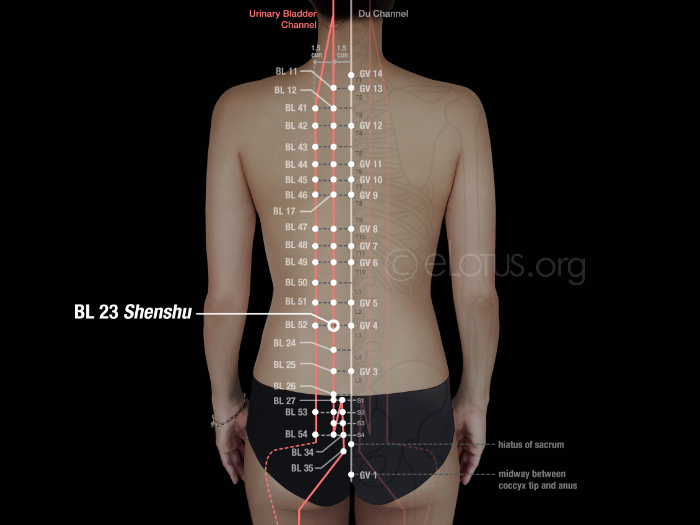
\includegraphics[width=0.25\linewidth]{images/image.png}
    \caption{Enter Caption}
    \label{fig:placeholder}
\end{figure}

\begin{figure}
    \centering
    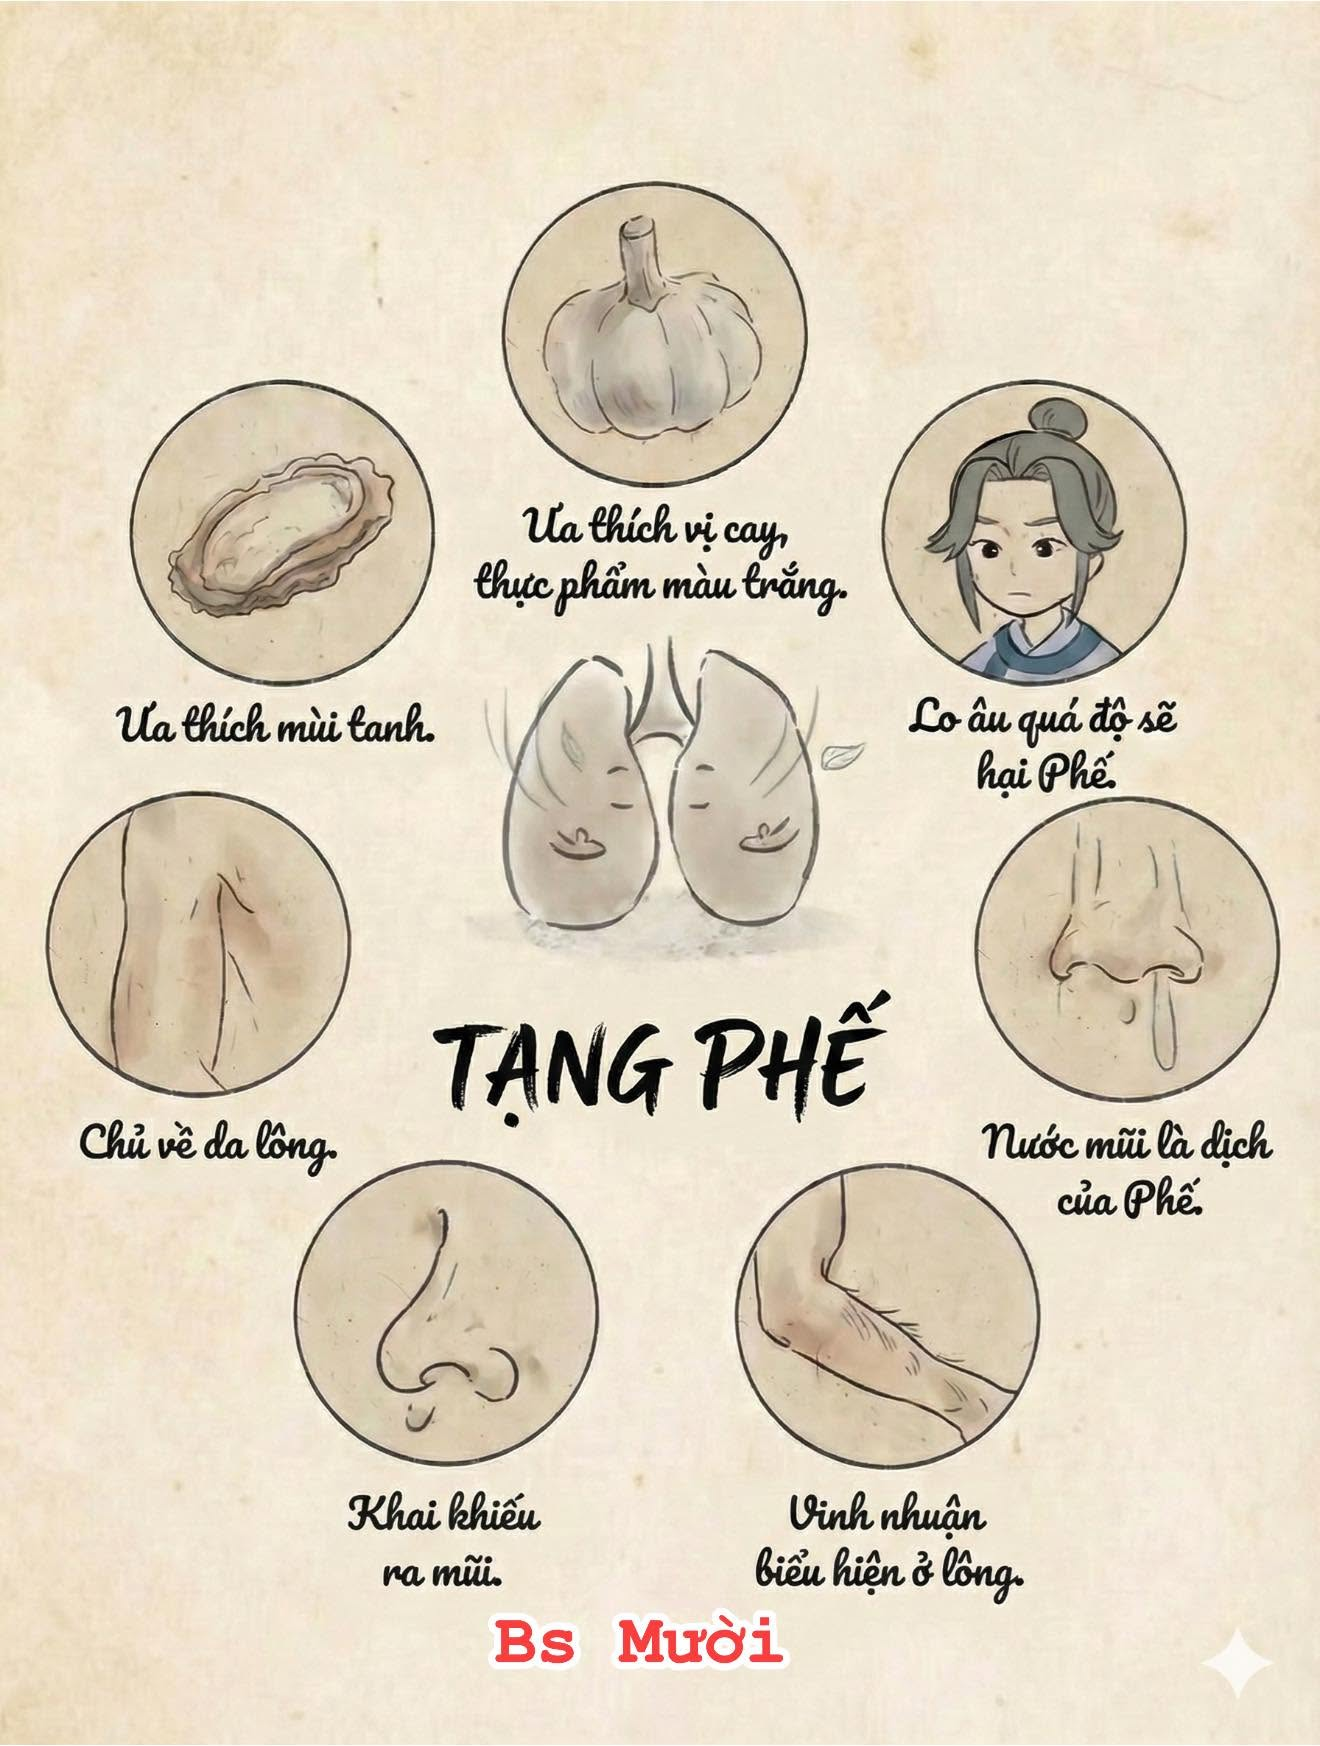
\includegraphics[width=0.25\linewidth]{images/tạng phế.png}
    \caption{Enter Caption}
    \label{fig:placeholder}
\end{figure}
\subsection{Phủ}
\subsection{Tương ứng ngũ hành}

Can
chủ về gân (nuôi dưỡng gân cốt) why, thể hiện ở móng chân móng tay (hồng nhuận) 
khai khiếu ở mắt
ngủ nghỉ máu về gan -> Gan bẩn (mỡ) -> máu bẩn

tạng tì hành thổ
Tiêu hoá thức ăn
suy dinh dưỡng -> chàn dịch ra ổ bụng
tì tốt -> giữ máu đi trong lòng mạch không bị thoát ra ngoài.
tì biểu hiện cơ nhục và tứ chi
miệng, môi (đỏ nhuận)

Phế
khí hô hấp, phân bổ khí huyết đi khắp cơ thể, bảo vệ cơ thể khai khiếu ở mũi.

Thận
hành thuỷ chủ cốt tuỷ, thận tốt xương khoẻ mạnh. giúp xương chắc khoẻ trí tuệ minh mẫn thông tuệ. chuyển hoá vitaminD chuyển hoá canxi vào xương.
Nạp khí (hen suyễn, chưã cả thận), chủ về cốt tuỷ (tuỷ đỏ chuyển hoá thành hồng cầu thì cần phải chuyển hoá từ hocmon tuyến thuận.), hấp thụ hồng cầu ngược lại, ...
khai khiếu ra tai ra đường đại tiện và 

Phủ chuyển hoá đồ ăn
Vị (dạ dày)
đởm túi mật (dịch mật)
Phủ tiểu trường

Phủ đại trường (tái hấp thu nước, tái hấp thu can xi)
bàng quang (chứ và 

Đởm

Tam tiêu

1. thượng tiêu
2. Trung tiêu
3. Hạ tiêu

Phủ kì hằng
1. não bể tuỷ (trí tuệ, trong cốt mạch)
2. tử cung (rỗng đặc)

\section{QUan hệ biểu lý (tạng và phủ)}
gan đổ vào mật mà mật đổ vào gan.

Phế đại tràng -> ung thư phổi hay bị táo bón, ảnh hưởng đến đại tràng.
thận bàng quang 

\section{Quan hệ giữa các tạng}
tim và thận không giao với nhau -> trên nóng dưới lạnh.
can và tì -> Quan hệ sơ tiết và tiêu hoá
phế và thận

Ứng dụng (dựa vào hiện tượng để chuẩn đoán bệnh)

\section{Ứng dụng trong điều trị}
- Tạng hay bồi bổ.
- Chữa bệnh bằng điều hoà tạng phủ

\section{Chuẩn đoán học yhct}
Tây y là cận lâm sàng.
Vọng văn vấn thiết.
chuẩn
đoán (đoán bệnh)

\subsection{tứ chuẩn}
vọng chuẩn
- vọng thần (sáng tỉnh táo ngôn ngữ rõ ràng)
- ít thần (mệt mỏi)
- mất thần (thần không còn nữa)

xem sắc mặt
- sắc đỏ (nhiệt chứng)
- sắc vàng (tì hư)
- sắc xanh (hàn, ứ huyết, động kinh)
- sác đen (thận hư, hàn chứng và ứ huyết)

Hình thái và động thái
- hình thể  
- động thái ()

Vọng về ngũ quan
- mắt
- mũi (phập phồng, chảy nước mũi, ...)
- môi (nhợt nhạt, thâm tím, khô nứt, ...)
- da (khô, )

Thiệt chẩn (chất lưỡi)
- lưỡi khô 
- lưỡi đỏ -> nhiệt , ứ huyết.
- lưỡi bệu -> từ hư
- tím ứ huyết -> ...

Rêu lưỡi
- trắng 
- xám đen -> ung thư

độ dày 
độ ẩm lưỡi

văn chẩn (nghe và ngửi)
- tiếng nói to thực chứng
- nhỏ
- thở gấp thô, yếu ngắn.
- ho đục, ho trong, ho khan.
- nấc liên tục mạnh yếu ngắt quãng.

Ngửi mùi chất tiết.
- mùi tanh hàn
- hơi thở hôi nhiệt
- nước tiểu ()
- phân khắm nông, tanh loãng

Thập vấn (10 điều hỏi)
1. hỏi về nóng lạnh (lạnh phát sốt, lạnh k....)
2. hỏi về mồ hôi ()
1. đại tiện
2. nước tiểu (trong  - hàn, nhiều - hàn)
3. ẩm thực ăn uống (ấm nóng, ngọt - tiểu đường). 
4. ngực bụng (có bị đau, sườn có căng hay không)
5. tai (có bị lãng tai hay không)
6. khát (thích uống nước ấm, hay lạnh, uống nhiều vẫn khát tiểu đường)
7. tiền xử bệnh.
8. nguyên nhân gây bệnh và người thân.

Thiết chuẩn (xem mặt, sờ lắn)
Án chuẩn (sờ nắn, mồ hôi dính, sờ bụng đau thực chứng - đau ruột thừa)
Sờ bụng thâý khối u....

\section{Bát cương}
biểu, lý, hư, thực, hàn, nhiệt, âm, dương

cương lĩnh biểu lý: bệnh ở nông hay sau
hàn nhiệt: hàn (thích ấm sợ lạnh, machj tri), nhiệt (..., hay bị táo bón)
hư thực: hư là suy kém, thực là thừa.
dương: là tổng cương (biểu thực nhiệt)
âm : (lý, hư hàn)

Biện chứng tạng phủ
Biện chứng tạng tâm và can. (Hồi hộp mất ngủ hay quên mặt nhơt)
Biện chứng tạng tì và phế.

\section{Nguyên nhân gây bệnh}
Mất cân bằng âm dương là nguyên nhân gây bệnh tật.

1. Ngoại (lục dâm lục tà, môi trường khí hậu tác động từ bên  ngoài, ,,,)
   Phong tà (gió) -> ,,, hay di chuyển 
   hàn lạnh -> sợ lạnh (tay chân lạnh)
   thử tà (nắng mùa hè)
   Thấp tà (ẩm thấp, ... , uể oải) 
   táo tà (độ khô), 
   hoả tà (nhiệt nóng)
   Lệ khí (dịch bệnh) -> thay đổi khí hâụ.
   
2. Nội (7 tình cảm)
    Hỷ Mừng quá hại tâm
    Nộ - giận dữ
    Tư - lo nghĩ, suy nghĩ
    
    
3. Bất ngoại nội nhân (ẩm thực ăn uống, lao động , tình dịch, muỗi đốt, ..., )
